\documentclass[a4paper,12pt]{extarticle}
\usepackage{algpseudocode}
\usepackage{geometry}
\usepackage[T1]{fontenc}
\usepackage[utf8]{inputenc}
\usepackage[english,russian]{babel}
\usepackage{amsmath}
\usepackage{amsthm}
\usepackage{amssymb}
\usepackage{fancyhdr}
\usepackage{setspace}
\usepackage{graphicx}
\usepackage{colortbl}
\usepackage{tikz}
\usepackage{pgf}
\usepackage{subcaption}
\usepackage{listings}
\usepackage{indentfirst}
\usepackage[
backend=biber,
style=numeric,
maxbibnames=99
]{biblatex}
\addbibresource{refs.bib}
\usepackage[colorlinks,citecolor=blue,linkcolor=blue,bookmarks=false,hypertexnames=true, urlcolor=blue]{hyperref} 
\usepackage{indentfirst}
\usepackage{mathtools}
\usepackage{booktabs}
\usepackage[flushleft]{threeparttable}
\usepackage{tablefootnote}

\usepackage{makecell}

\usepackage{chngcntr} % нумерация графиков и таблиц по секциям
\counterwithin{table}{section}
\counterwithin{figure}{section}

\graphicspath{{graphics/}}%путь к рисункам

\makeatletter
% \renewcommand{\@biblabel}[1]{#1.} % Заменяем библиографию с квадратных скобок на точку:
\makeatother

\geometry{left=2.5cm}% левое поле
\geometry{right=1.0cm}% правое поле
\geometry{top=2.0cm}% верхнее поле
\geometry{bottom=2.0cm}% нижнее поле
\setlength{\parindent}{1.25cm}
\renewcommand{\baselinestretch}{1.5} % междустрочный интервал


\newcommand{\bibref}[3]{\hyperlink{#1}{#2 (#3)}} % biblabel, authors, year
\addto\captionsrussian{\def\refname{Список литературы (или источников)}} 

\renewcommand{\theenumi}{\arabic{enumi}}% Меняем везде перечисления на цифра.цифра
\renewcommand{\labelenumi}{\arabic{enumi}}% Меняем везде перечисления на цифра.цифра
\renewcommand{\theenumii}{.\arabic{enumii}}% Меняем везде перечисления на цифра.цифра
\renewcommand{\labelenumii}{\arabic{enumi}.\arabic{enumii}.}% Меняем везде перечисления на цифра.цифра
\renewcommand{\theenumiii}{.\arabic{enumiii}}% Меняем везде перечисления на цифра.цифра
\renewcommand{\labelenumiii}{\arabic{enumi}.\arabic{enumii}.\arabic{enumiii}.}% Меняем везде перечисления на цифра.цифра

\newcommand*{\approxident}{%
  \mathrel{\vcenter{\offinterlineskip
  \hbox{$\sim$}\vskip-.35ex\hbox{$\sim$}\vskip-.35ex\hbox{$\sim$}}}}

\begin{document}
\input{title_vkr}% это титульный лист - выберите подходящий вам из имеющихся в проекте вариантов (kr - курсовая работа у 3 курса, vkr - выпускная квалификационная работа у 4 курса)
\newpage
\setcounter{page}{2}

{
	\hypersetup{linkcolor=black}
	\tableofcontents
}

\newpage

\newpage
\section*{Аннотация}   % this is how to use russian
В данной работе исследуется дифференциально-геометрический подход к анализу данных на примере обработки результатов магнитно-резонансной томографии (МРТ). Основное внимание уделяется применению методов римановой геометрии в вероятностных пространствах для построения геометрических и топологических структур на выборках данных с использованием диффузионных операторов.
Рассматриваются вычислительные аспекты метода, его устойчивость к шуму и эффективность в сравнении с традиционными методами снижения размерности, такими как PCA, Isomap, MDS и другими. Особый акцент сделан на возможностях дифференциальной геометрии в выявлении скрытых закономерностей в многомерных медицинских данных, что может способствовать более точной диагностике и анализу структурных изменений в головном мозге.
Полученные результаты показывают, что дифференциально-геометрические методы обладают высокой точностью в описании сложных пространственных структур и представляют собой перспективный инструмент для анализа медицинских изображений и задач машинного обучения в медицине.

\section*{Ключевые слова}
Дифференциальная геометрия, риманова геометрия, анализ данных, топологический анализ данных, многомерные данные.
\pagebreak

\section{Введение}   % this is how to use russian

Современные методы анализа данных всё чаще опираются на математические модели, позволяющие учитывать их сложную геометрическую и топологическую структуру. В этом контексте дифференциальная геометрия предоставляет мощный инструмент для изучения многомерных данных, представляя их в виде многообразий и исследуя их свойства с помощью римановой геометрии и операторов дифференциального исчисления.

Одним из перспективных направлений является диффузионная геометрия, которая использует методы теории вероятностей и операторов Маркова для построения геометрических объектов в пространстве данных. Такой подход позволяет не только выявлять скрытые закономерности, но и делать это с высокой устойчивостью к шуму и вычислительной эффективностью. В отличие от традиционных методов, основанных на локальном разложении главных компонент или устойчивых гомологиях, диффузионная геометрия обеспечивает более глубокое описание структуры данных, что делает её особенно полезной в задачах машинного обучения, визуализации и статистического анализа.

Одной из важных областей применения данного подхода является анализ медицинских данных, в частности, магнитно-резонансной томографии (МРТ). Традиционные методы обработки данных имеют ограниченную способность к выявлению сложных нелинейных зависимостей в данных. Использование дифференциально-геометрического подхода позволяет построить топологические и геометрические структуры на основе данных МРТ, что способствует более точному выявлению патологий, анализу изменений в структурах головного мозга и повышению качества диагностики. Применение таких методов может значительно улучшить точность медицинских решений, обеспечивая новый уровень интерпретации данных за счет использования информации о геометрии и топологии изображений.

Помимо дифференциально-геометрического подхода, в данной работе мы рассмотрим и другие популярные методы анализа многомерных данных, такие как Isomap, MDS, PCA и другие алгоритмы нелинейного уменьшения размерности. Эти методы широко применяются для выявления низкоразмерной структуры в многомерных данных и позволяют эффективно решать задачи визуализации, кластеризации и классификации. Однако, несмотря на их популярность, они обладают рядом ограничений, включая зависимость от выбора метрик, чувствительность к шуму и ограниченные возможности в описании сложных топологических структур.

В связи с этим актуальной задачей является сравнение дифференциально–геометрического подхода с традиционными методами анализа данных, а также исследование его вычислительных аспектов, устойчивости и возможностей в задачах машинного обучения. Ожидается, что применение диффузионной геометрии позволит получить более точные и информативные представления многомерных данных, а также предложить новые способы их анализа и интерпретации.

Итого, данной работе мы будем рассматривать ключевые принципы дифференциально-геометрического подхода к анализу данных, включая построение векторных полей, дифференциальных форм и операторов внешнего дифференцирования на выборках данных. Мы исследуем их вычислительные аспекты, устойчивость к шуму и практическое применение для изучения многомерных структур. В конечном итоге мы покажем, как дифференциально-геометрические методы могут улучшить анализ сложных данных и предоставить новые инструменты для их интерпретации.

Для выполнения такой задачи необходимо выполнить следующие шаги:

\begin{enumerate}
    \item Изучить теоретические основы дифференциально-геометрического подхода к анализу данных, включая риманову и диффузионную геометрию;
    \item Рассмотреть методы построения геометрических структур в вероятностных пространствах и их применение к выборкам данных;
    \item Разработать или адаптировать алгоритмы вычисления векторных полей, дифференциальных форм и операторов внешнего дифференцирования на многомерных данных;
    \item Провести сравнительный анализ диффузионной геометрии с традиционными методами, такими как локальный метод главных компонент и метод устойчивых гомологий;
    \item Провести экспериментальное сравнение дифференциально-геометрических методов с Isomap, MDS, PCA и другими, анализируя их точность, вычислительную сложность и устойчивость к шуму;
    \item Реализовать и протестировать предложенные методы на реальных и синтетических наборах данных;
    \item Проанализировать результаты и определить перспективы дальнейшего применения дифференциально–геометрических методов в анализе данных.
\end{enumerate}

\section{Постановка задачи}   % this is how to use russian

В работе мы рассматриваем задачу применения дифференциально–геометрического подхода к анализу данных и его сравнения с традиционными методами нелинейного уменьшения размерности, например, Isomap, MDS, PCA и другие. Для этого необходимо разработать и реализовать методологию построения геометрических структур в вероятностных пространствах и изучить их вычислительные и статистические свойства.

Первым этапом является формализация математической модели, позволяющей использовать дифференциально-геометрические инструменты для обработки выборок данных. В частности, требуется определить, каким образом можно вычислять векторные поля, дифференциальные формы и операторы внешнего дифференцирования, опираясь на структуру римановых многообразий и диффузионную геометрию.

После разработки теоретических основ необходимо реализовать предложенные методы на практике. Для этого требуется создать программную реализацию вычислительных алгоритмов, позволяющих строить дифференциально-геометрические представления данных. Отдельной важной задачей на этом этапе является выбор оптимальных численных методов, которые обеспечивают устойчивость вычислений и высокую точность.

Следующим этапом является сравнительный анализ дифференциально-геометрического подхода с традиционными методами анализа данных. Здесь необходимо учесть ключевые аспекты, такие как вычислительная сложность, устойчивость к шуму, способность выявлять глобальные и локальные структуры в данных, а также эффективность в задачах визуализации и классификации. Дополнительно требуется провести эксперименты на синтетических и реальных наборах данных, чтобы оценить практическую применимость различных методов. Это позволит выявить их сильные и слабые стороны, а также определить области, в которых дифференциальная геометрия имеет явные преимущества перед традиционными методами.

Финальным этапом работы является обобщение полученных результатов и формулирование выводов о перспективности дифференциально-геометрического подхода для анализа сложных многомерных данных.

В конечном итоге мы хотим получить фреймворк, которые принимает на вход пространство точек, полученных в результате МРТ сканирования, а на выходе получает изображения с выделенными аномалиями. В контексте МРТ-снимков аномалией может являться некая особенность в структуре мозга, например, опухоли, кисты, гематомы и так далее. Данную задачу уже можно решить с помощью методов компьютерного зрения (computer vision, CV), но данные методы зачастую выделяют либо слишком много, либо неправильные области (пример выделения областей можно увидеть на рисунке ~\ref{fig:mri_internal_structures_detection}), а в данной работе мы хотим ориентировать не на изображение объектов на снимке, а на расположение точек в пространстве. 

\begin{figure}[ht]
  \centering
  \begin{minipage}[b]{0.9\linewidth} 
    \centering
    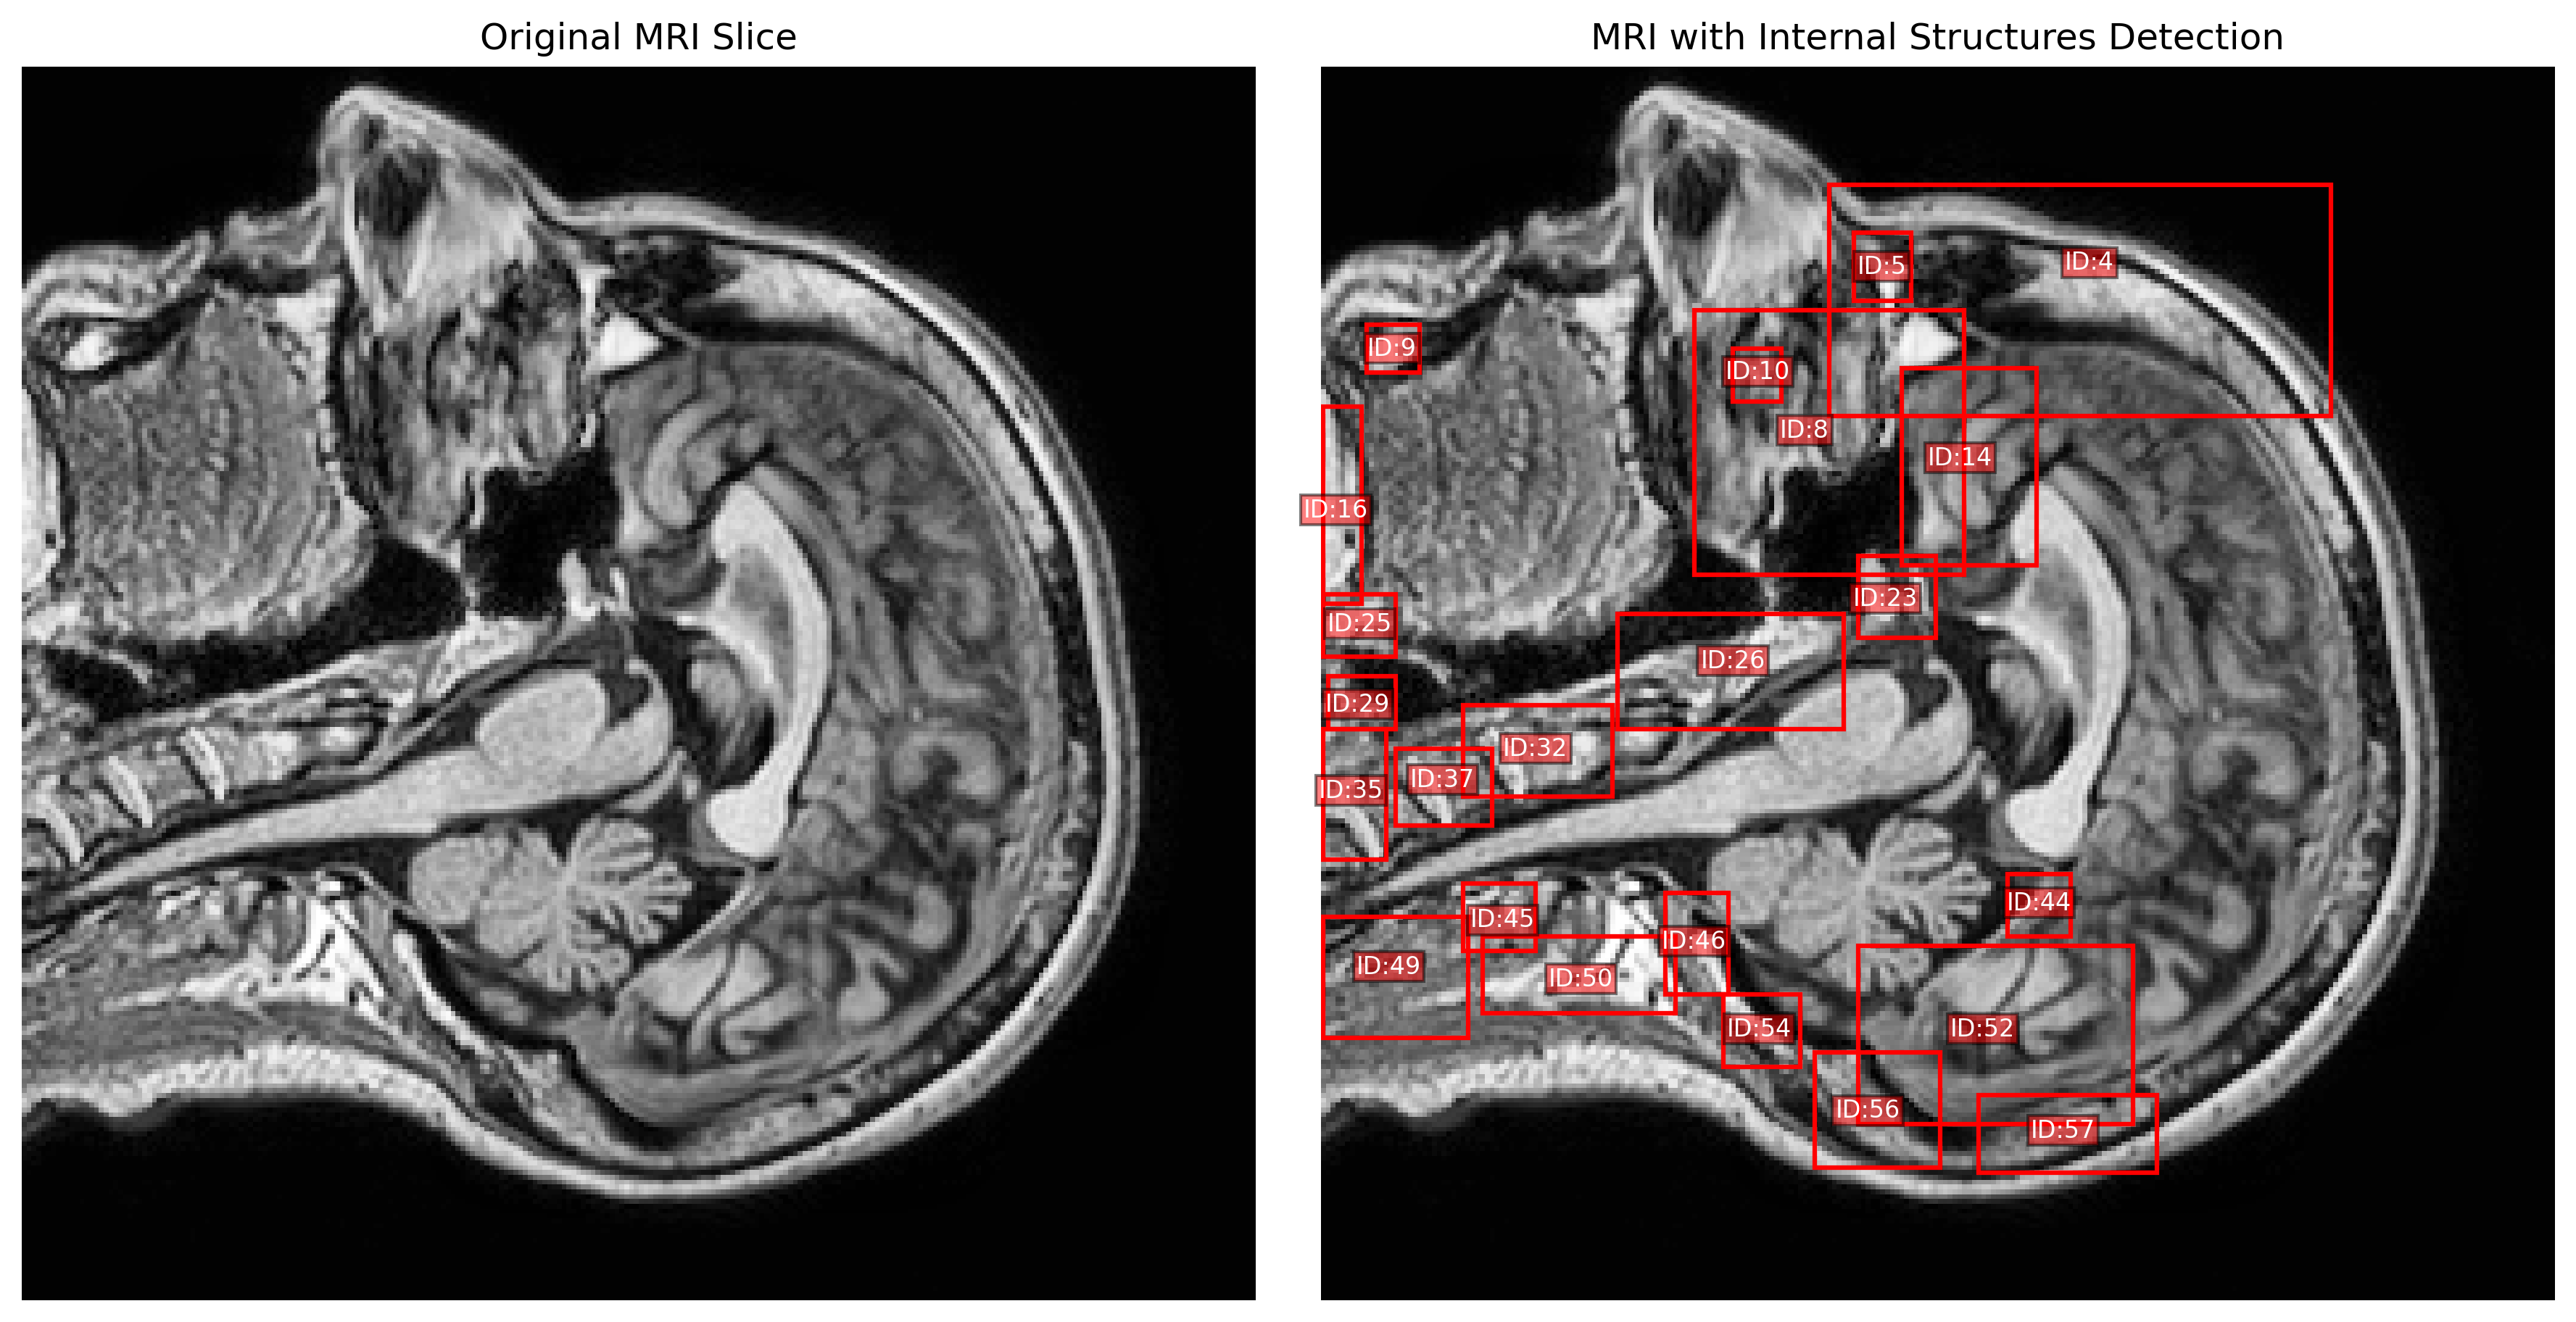
\includegraphics[width=\linewidth]{mri_internal_structures_detection}
    \caption{Визуализация детекции с помощью методов компьютерного зрения}
    \label{fig:mri_internal_structures_detection}
  \end{minipage}
\end{figure}

\section{Обзор литературы}

\subsection{Основные термины, определения и сокращения}

\textit{Isomap} – метод многомерного шкалирования, который используется для понижения размерности данных и визуализации их в низкоразмерном пространстве, сохраняя при этом геодезические расстояния между точками данных.

\textit{LLE} – Locally Linear Embedding, метод снижения размерности данных, который стремится сохранить локальные структуры данных в низкоразмерном пространстве. Основан на предположении о том, что данные, близкие в исходном пространстве, должны оставаться близкими и в целевом пространстве низкой размерности.

\textit{MDS} – Multidimensional Scaling, метод анализа данных, который используется для визуализации и понижения размерности данных, сохраняя при этом относительные расстояния между точками данных.

\textit{PCA} – Principal Component Analysis, статистический метод анализа данных, используемый для сокращения размерности данных путем выявления и использования наиболее информативных признаков или компонентов в наборе данных.

\textit{t-SNE} – t-Distributed Stochastic Neighbor Embedding, метод нелинейного снижения размерности данных и визуализации высокоразмерных данных в двумерное или трехмерное пространство для удобного восприятия и анализа.

\textit{UMAP} – Uniform Manifold Approximation and Projection, метод машинного обучения и анализа данных, который используется для понижения размерности данных и визуализации их в низкоразмерном пространстве, сохраняя при этом глобальную структуру и локальные отношения между данными.

\textit{{$\Gamma$}-исчисление (Bakry-Émery {$\Gamma$}-calculus)} – формализм, используемый для анализа свойств марковских процессов и построения геометрических объектов на вероятностных пространствах, что позволяет переносить концепции римановой геометрии на случайные выборки данных.

\textit{Дифференциальная геометрия в анализе данных} – область математики, изучающая геометрические свойства данных с использованием понятий римановой геометрии, таких как кривизна, дифференциальные формы и операторы внешнего дифференцирования. Включает методы построения геометрических структур на основе стохастических процессов.

\textit{Диффузионная карта (Diffusion Map)} – метод нелинейного снижения размерности, основанный на анализе спектральных свойств стохастического процесса диффузии, распространяющегося по данным. Используется для выявления скрытых структур в многомерных выборках.

\textit{Устойчивые гомологии (Persistent Homologies)} – метод топологического анализа данных, позволяющий выявлять устойчивые многомерные структуры в выборках данных. Используется в задачах кластеризации и выявления сложных топологических особенностей данных.

\textit{Риманова геометрия} — раздел дифференциальной геометрии, изучающий геометрические свойства многообразий с заданной римановой метрикой, которая определяет скалярное произведение векторов в каждой точке.

\subsection{Обзор методов понижения размерности}

Для сравнения методов дифференциально-геометрического подхода к анализу
данных, нам необходимо изучить методы понижения размерности, как уже существующие методы решения задачи. Для этого мы проанализировали статьи [1] с описанием работы метода PCA, статью [2] с описанием работы метода t-SNE, статью [3] с описанием работы метода LDA, статью [4] с описанием работы метода LLE и статью [5] со сравнением вышеуказанных методов с рядом других методов понижения размерности, в частности UMAP, MDS и Isomap. В приведенных выше статьях не проводились эксперименты со сравнением этих методов с  дифференциально-геометрическим подходом, поэтому мы ничего не можем сказать об ожидаемых результатах. Тем не менее мы считаем, что каждый из этих методов может быть полезен в рамках текущей задачи, и поэтому мы должны провести самостоятельные эксперименты. 

\subsection{Сравнение методов понижения размерности}

Если переходить к более подробному сравнению, среди наиболее известных методов, используемых для этих целей, можно выделить PCA (Principal Component Analysis) и Isomap (Isometric Mapping).

PCA является классическим методом линейного снижения размерности, который используется для выявления направлений с наибольшей дисперсией в данных, что позволяет сохранить основную информацию, сокращая количество признаков [6]. Однако PCA ограничен только линейными преобразованиями и не может эффективно обрабатывать нелинейные структуры данных.

Для работы с нелинейными структурами был разработан метод Isomap [7], который сохраняет геодезические расстояния между точками в низкоразмерном пространстве. Это позволяет использовать Isomap для анализа данных, лежащих на многообразиях, и успешно применяться в задачах визуализации и кластеризации данных. Isomap, в отличие от PCA, является нелинейным методом, поэтому теоретические он должен лучше сохранять глобальную структуру данных, особенно если они лежат на многообразиях. Однако Isomap требует выбора параметра k (число ближайших соседей), который чувствителен к шуму и вычислительно сложнее [8].

Другим методом снижения размерности является MDS (Multidimensional Scaling), который минимизирует ошибки реконструкции попарных расстояний в данных, преобразуя их в низкоразмерное пространство [9]. MDS универсален и применим для визуализации как линейных, так и нелинейных данных. Однако его производительность и точность зависят от используемой метрики.

Среди современных методов снижения размерности данных можно выделить t-SNE (t-Distributed Stochastic Neighbor Embedding), LDA (Latent Dirichlet Allocation), LLE (Locally Linear Embedding) и UMAP (Uniform Manifold Approximation and Projection). Каждый из них обладает уникальными свойствами и применяется в различных задачах анализа данных.

Метод t-SNE широко используется для визуализации многомерных данных в низкоразмерном пространстве. Он основан на стохастическом сохранении локальных структур, что позволяет эффективно группировать данные по кластерам. Однако существенным недостатком t-SNE является его вычислительная сложность, из-за которой метод плохо масштабируется на большие объемы данных. Кроме того, он не сохраняет глобальную структуру, что может затруднить интерпретацию результатов [2].

Метод LLE предлагает другой подход к снижению размерности, стремясь сохранить локальные линейные структуры данных. В отличие от t-SNE, он работает детерминировано и позволяет строить более интерпретируемые представления данных. Однако его недостатком является высокая чувствительность к шуму и зависимость от выбора параметра количества соседей, что может приводить к искажениям при неправильной настройке модели [10]. На практике это означает, что метод сложно назвать универсальным, так как он требует тщательной настройки.

UMAP является современной альтернативой t-SNE, предлагая схожее качество визуализации, но при этом обладая значительно лучшей вычислительной эффективностью [11]. Метод базируется на аппроксимации локальной и глобальной структуры данных с использованием теоретико-графового подхода. Одним из главных преимуществ UMAP является его способность сохранять как локальные, так и глобальные свойства данных, что делает его более универсальным инструментом для анализа многомерных структур. Тем не менее UMPA имеет ряд недостатков: он плохо масштабируем на размерность пространства, количество данных и число ближайших соседей, а так же требует большого количества ресурсов и имеет недостатки воспроизводимости результатов.

Таким образом, мы можем сделать вывод, что выбор метода снижения размерности зависит от конкретной задачи, а значит дифференциально-геометрические методы будет необходимо сравнить с каждым из них.

\subsection{Топологические методы анализа данных}

Топологические методы анализа данных (Topological Data Analysis, TDA) представляют собой мощный инструментарий для выявления глобальной структуры сложных многомерных данных [12]. Эти методы основаны на топологических инвариантах, таких как гомологии и когомологии, которые позволяют находить устойчивые структуры в данных, инвариантные к малым возмущениям. Одним из ключевых преимуществ TDA является его способность работать с данными, представленными в виде точечных облаков, без необходимости задавать явную метрическую структуру.

Одним из наиболее распространенных методов TDA является устойчивые гомологии [13]. Этот метод позволяет анализировать, как изменяются топологические свойства данных при варьировании масштаба. В частности, строятся так называемые персистентные диаграммы, которые отражают устойчивые топологические структуры, такие как компоненты связности, циклы, полости и так далее. В статье [14] показано, как устойчивые гомологии применяется в биологии, медицине, обработке изображений и машинном обучении для выявления сложных структурных закономерностей в данных, а значит может быть релевантная для нашей задачи. Устойчивые гомологии основывается на построении так называемой фильтрации компонентов, при которой постепенно добавляются новые связи между точками, начиная от разрозненных точек до полного графа. На каждом этапе этой фильтрации вычисляются гомологические группы, отражающие топологические свойства данных, и отслеживаются изменения этих групп по мере увеличения масштаба. Основная идея заключается в том, что устойчивые (персистентные) топологические особенности, такие как долгоживущие компоненты связности и циклы, являются важными характеристиками структуры данных, в то время как ``кратковременные'' особенности могут рассматриваться как шум.

\subsection{Теория Морса и графы Риба}

Другим важным направлением топологического анализа данных является использование теории Морса и графов Риба [15]. Эти методы позволяют восстанавливать топологическую структуру данных путем построения упрощенного представления их многомерного распределения. В частности, графы Риба используются для выявления кластеров и разбиения данных на смысловые регионы, что делает их полезными в задачах визуализации и классификации. Более подробно, в контексте анализа данных это позволяет выявлять ключевые топологические изменения в многомерных данных при изменении параметров или уровня значений функции. Например, при использовании функции плотности вероятности можно изучать, как связные компоненты данных объединяются или разрываются при изменении уровня плотности. Такие исследования помогают выделять кластеры, сегментировать данные или строить обобщенные представления сложных структур.

В свою очередь графы Риба, основанные на теории Морса, используются для представления топологической структуры данных в виде упрощенного графа. Узлы этого графа соответствуют критическим точкам функции Морса, а рёбра — изменениям топологической структуры между этими точками. Графы Риба обеспечивают наглядное и компактное представление глобальной структуры данных, что делает их особенно полезными для анализа многомерных распределений, где визуализация в исходном пространстве затруднена.

\subsection{Использование топологических векторов для снимков МРТ}

Существует также направление, связанное с построением топологических векторов признаков для машинного обучения. Данный метод был подробно описан в статье [16]. В этом подходе персистентные диаграммы кодируются в числовые признаки, которые затем используются в алгоритмах классификации и кластеризации. Такие методы успешно применяются, например, для анализа МРТ-снимков в медицине, где топологические характеристики изображений помогают выявлять особенности и улучшать точность диагностики.

Основная идея данного подхода заключается в том, чтобы преобразовать топологические сведения, полученные с помощью методов TDA, в форму, удобную для работы с классическими алгоритмами машинного обучения. Это достигается с помощью различных стратегий кодирования, например, в них могут использовать персистентные изображения, персистентные ландшафты, персистентные гистограммы и персистентные кривые. Эти представления позволяют свести топологические инварианты, такие как устойчивые циклы и компоненты связности, к числовым векторным признакам, пригодным для использования в таких методах, как SVM, случайные леса и нейронные сети.

Таким образом, мы можем сделать вывод, что топологические методы анализа данных представляют собой перспективное направление в современной науке о данных. Их преимущества заключаются в высокой устойчивости к шуму и способности выявлять сложные нелинейные структуры, которые трудно обнаружить с помощью традиционных статистических и геометрических методов, а значит данные методы могут быть полезны при анализе данных МРТ исследований. 

\section{Сравнение методов понижения размерности на примере результатов МРТ}

\subsection{Выбор и загрузка датасета}

Для демонстрации работы и сравнения методов мы выбрали датасет\footnote{Датасет доступен по ссылке: \url{https://brain-development.org/ixi-dataset/}, дата обр. 27.01.2025} с МРТ изображениями головного мозга более чем 500 здоровых добровольцев. После загрузки и векторизации данных можно применить различные методы понижения размерности для визуализации и анализа. 

Для сбора датасета авторы провели исследования в трех разных больницах Лондона:
больнице Hammersmith Hospital с использованием системы Philips 3T, 
больнице Guy’s Hospital с использованием системы Philips 1.5T и
институте психиатрии (Institute of Psychiatry) с использованием системы GE 1.5T. В результате были получены изображения T1-взвешенной (T1-weighted, T1W) МРТ –  тип магнитно-резонансных снимков, в которых контрастность определяется продольной (T1) релаксацией тканей. T1-взвешенная МРТ используется для оценки анатомии мозга, выявления опухолей, кровоизлияний и атрофии тканей, то есть дальнейший анализ таких изображений может играть важную роль в медицинской среде. 

\subsection{Сравнение методов понижения размерности}

На основе данных из датасета с МРТ снимками мы построили разбиение на кластеры с помощью популярных методов понижения размерности. Результаты разбиения можно увидеть на рисунках ~\ref{fig:pca}, ~\ref{fig:tsne}, ~\ref{fig:umap}, ~\ref{fig:mds}, ~\ref{fig:lle}, ~\ref{fig:isomap}, ~\ref{fig:lda}

\begin{figure}[ht]
  \centering
  \begin{minipage}[b]{0.45\linewidth} 
    \centering
    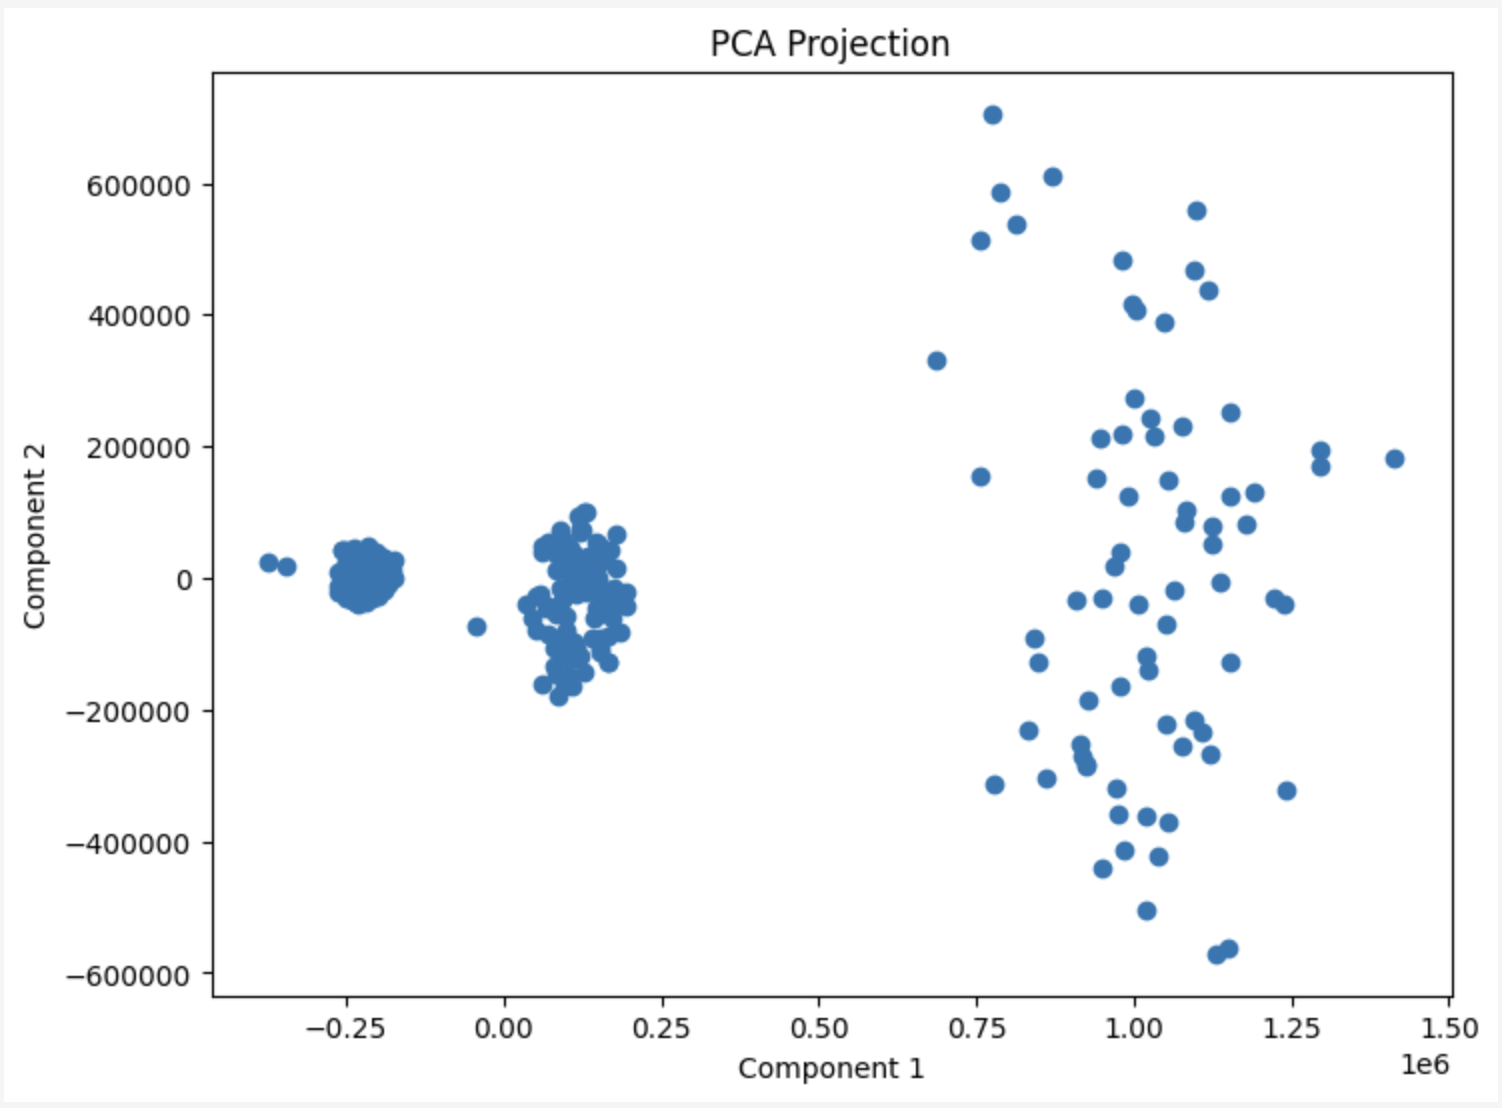
\includegraphics[width=\linewidth]{pca_proj.png}
    \caption{PCA при n\_components=2}
    \label{fig:pca}
  \end{minipage}
  \hspace{0.05\linewidth} 
  \begin{minipage}[b]{0.45\linewidth}
    \centering
    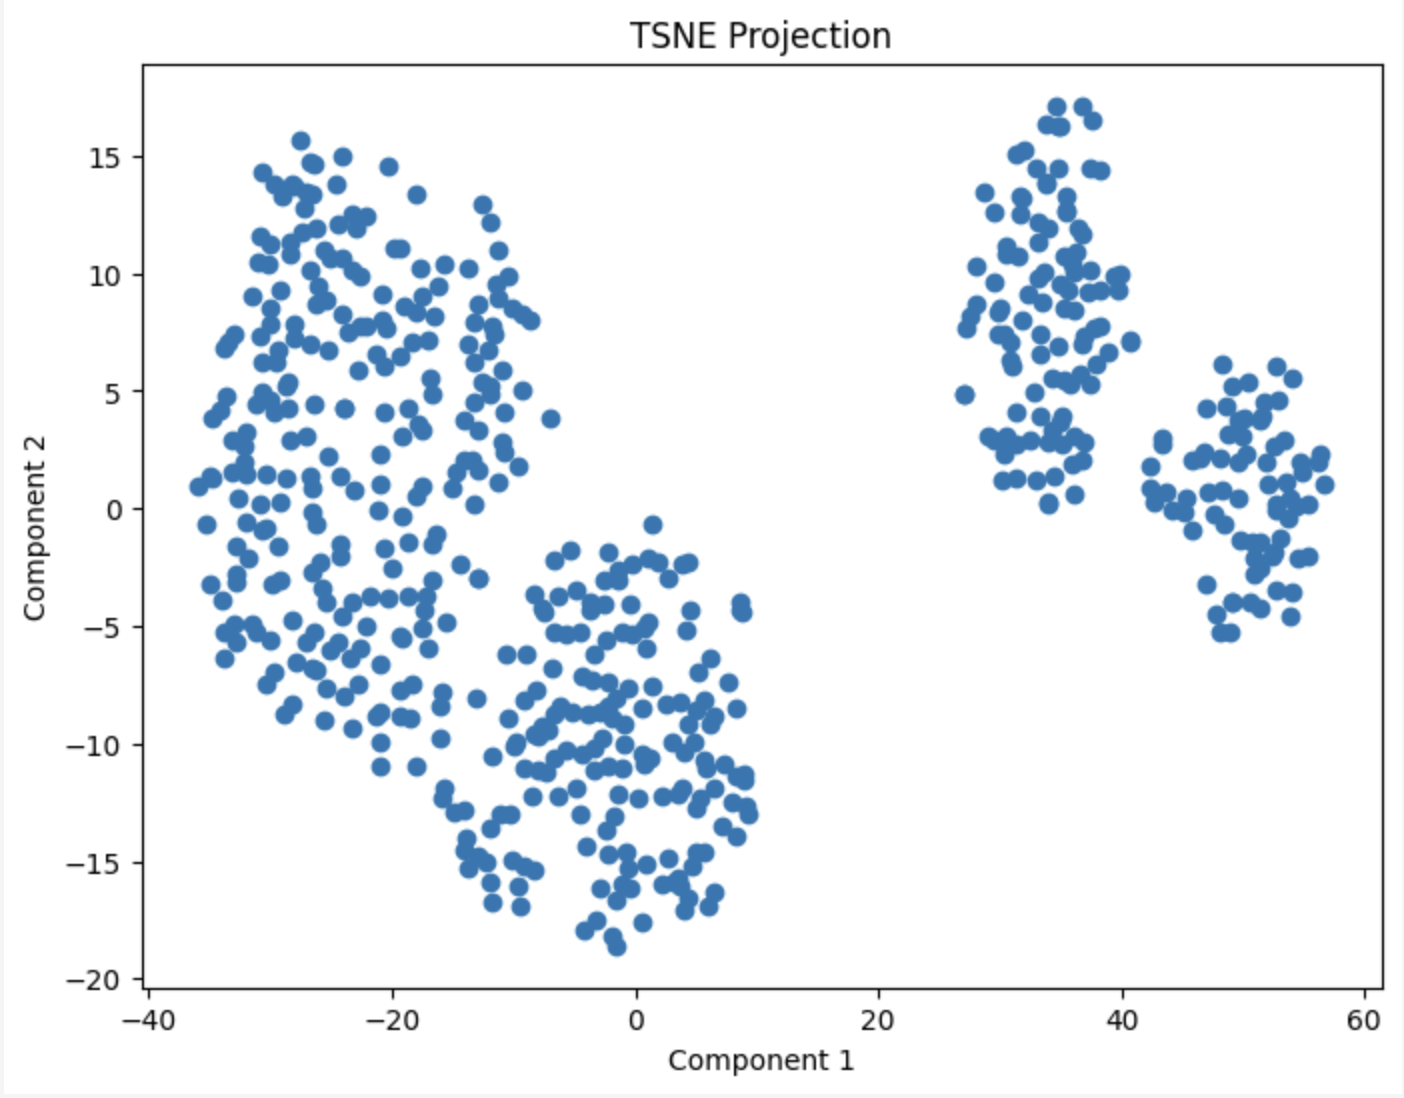
\includegraphics[width=\linewidth]{tsne_proj.png}
    \caption{t-SNE при n\_components=2}
    \label{fig:tsne}
  \end{minipage}
\end{figure}

\begin{figure}[ht]
  \centering
  \begin{minipage}[b]{0.45\linewidth} 
    \centering
    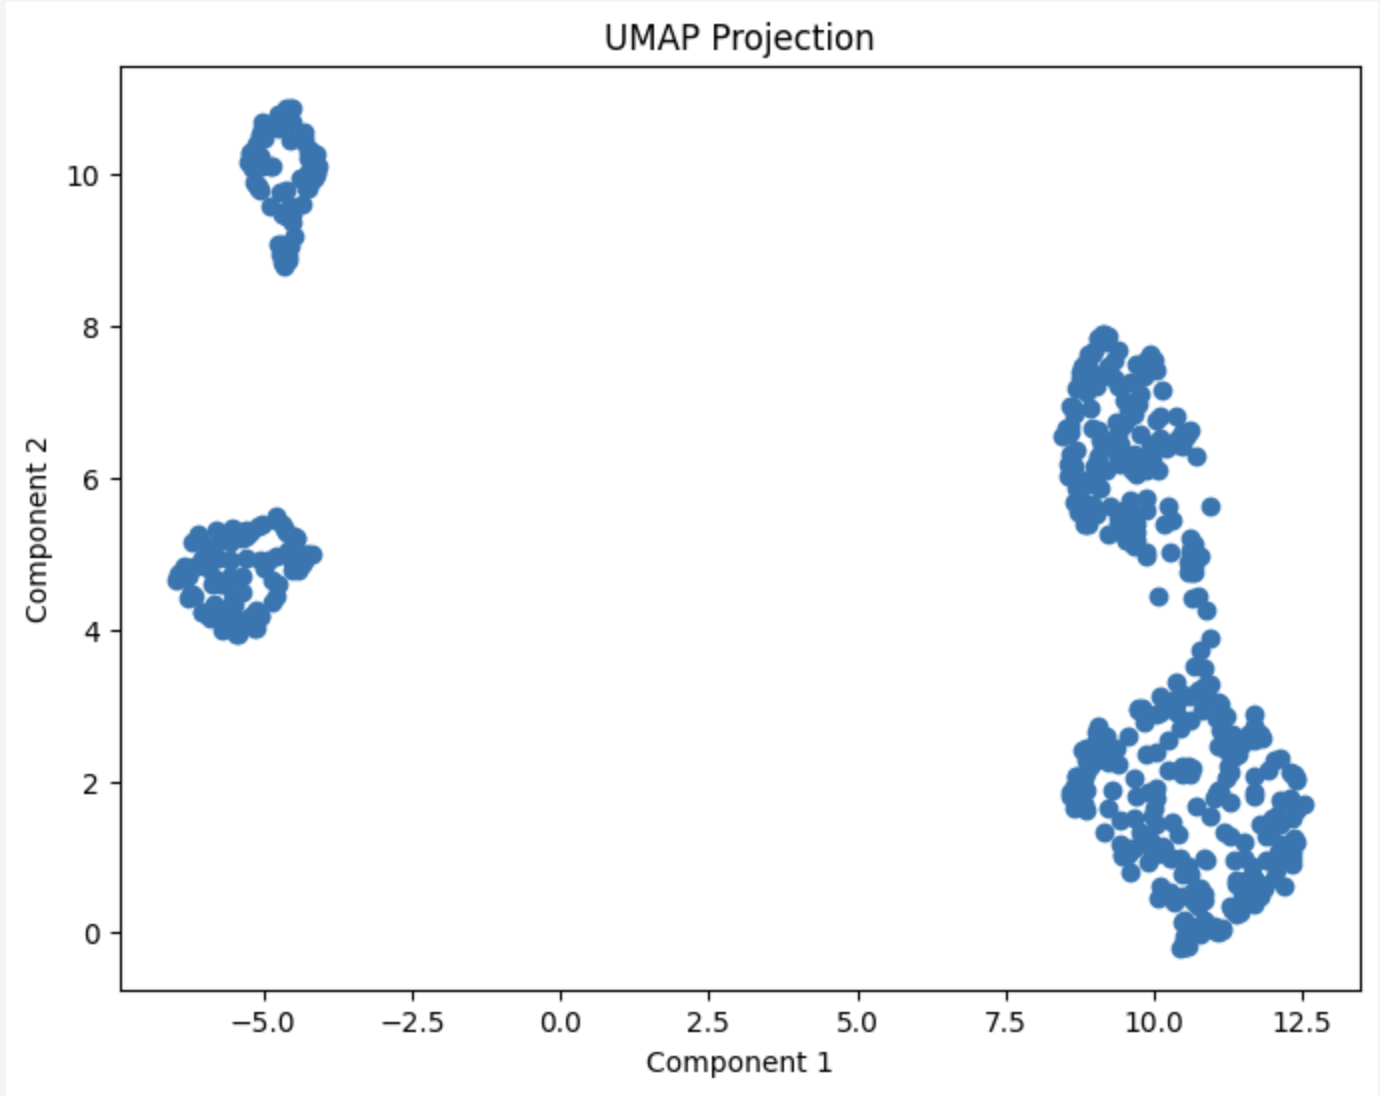
\includegraphics[width=\linewidth]{umap_proj.png}
    \caption{UMAP при n\_components=2}
    \label{fig:umap}
  \end{minipage}
  \hspace{0.05\linewidth} 
  \begin{minipage}[b]{0.45\linewidth}
    \centering
    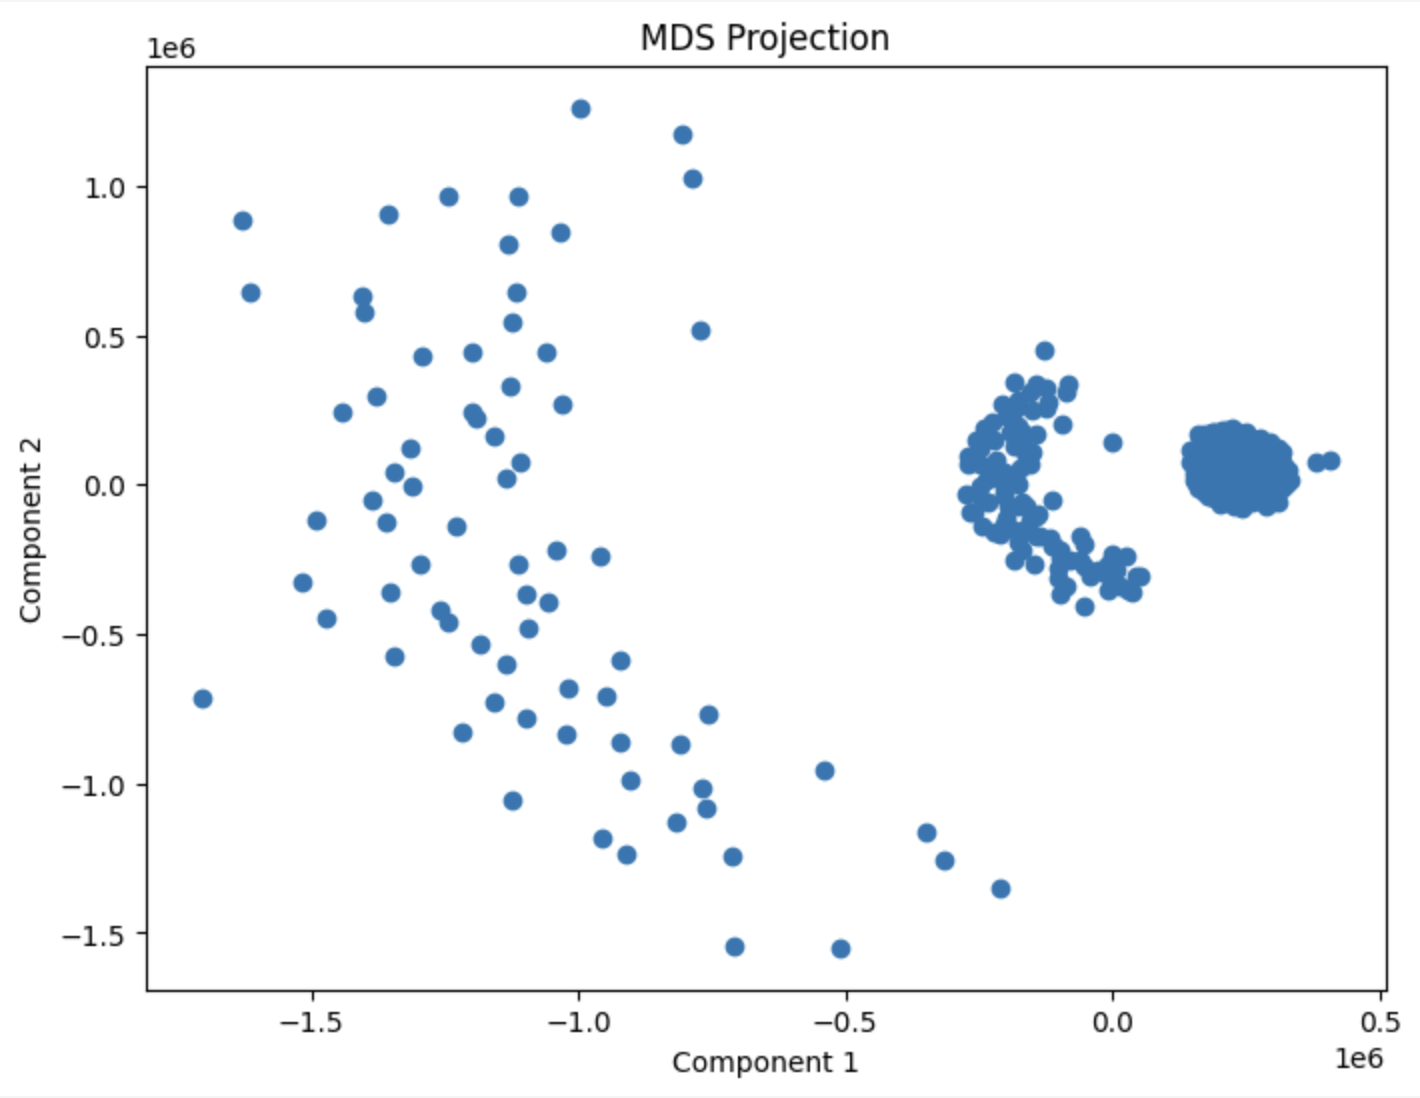
\includegraphics[width=\linewidth]{mds_proj.png}
    \caption{MDS при n\_components=2}
    \label{fig:mds}
  \end{minipage}
\end{figure}

\begin{figure}[ht]
  \centering
  \begin{minipage}[b]{0.45\linewidth} 
    \centering
    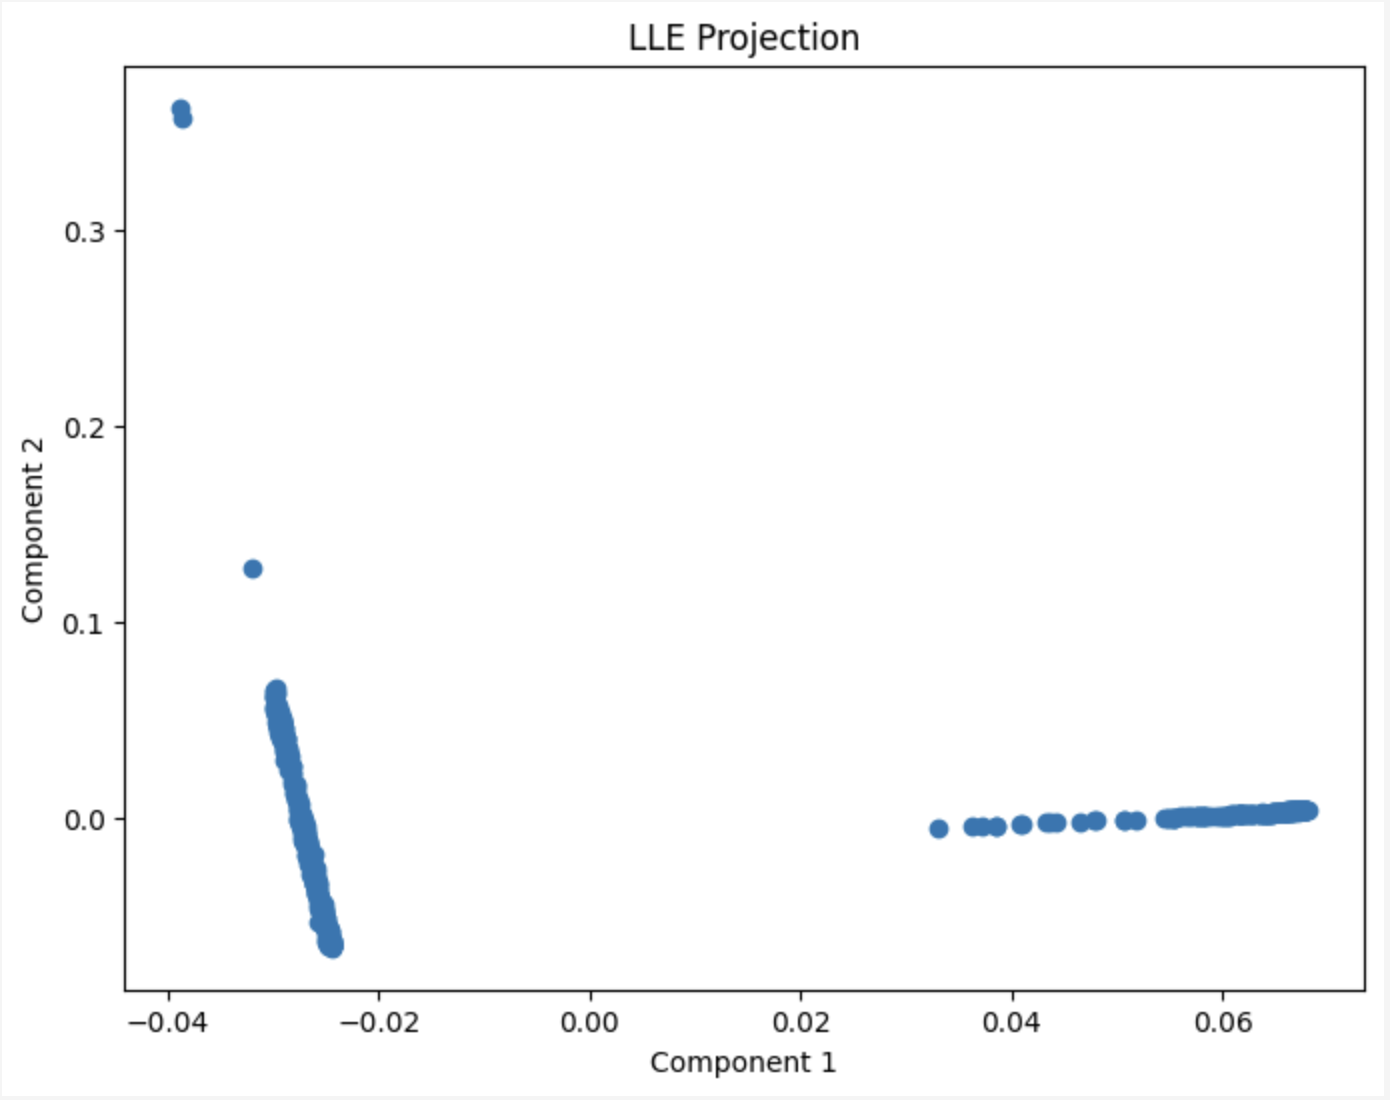
\includegraphics[width=\linewidth]{lle_proj.png}
    \caption{LLE при n\_components=2}
    \label{fig:lle}
  \end{minipage}
  \hspace{0.05\linewidth} 
  \begin{minipage}[b]{0.45\linewidth}
    \centering
    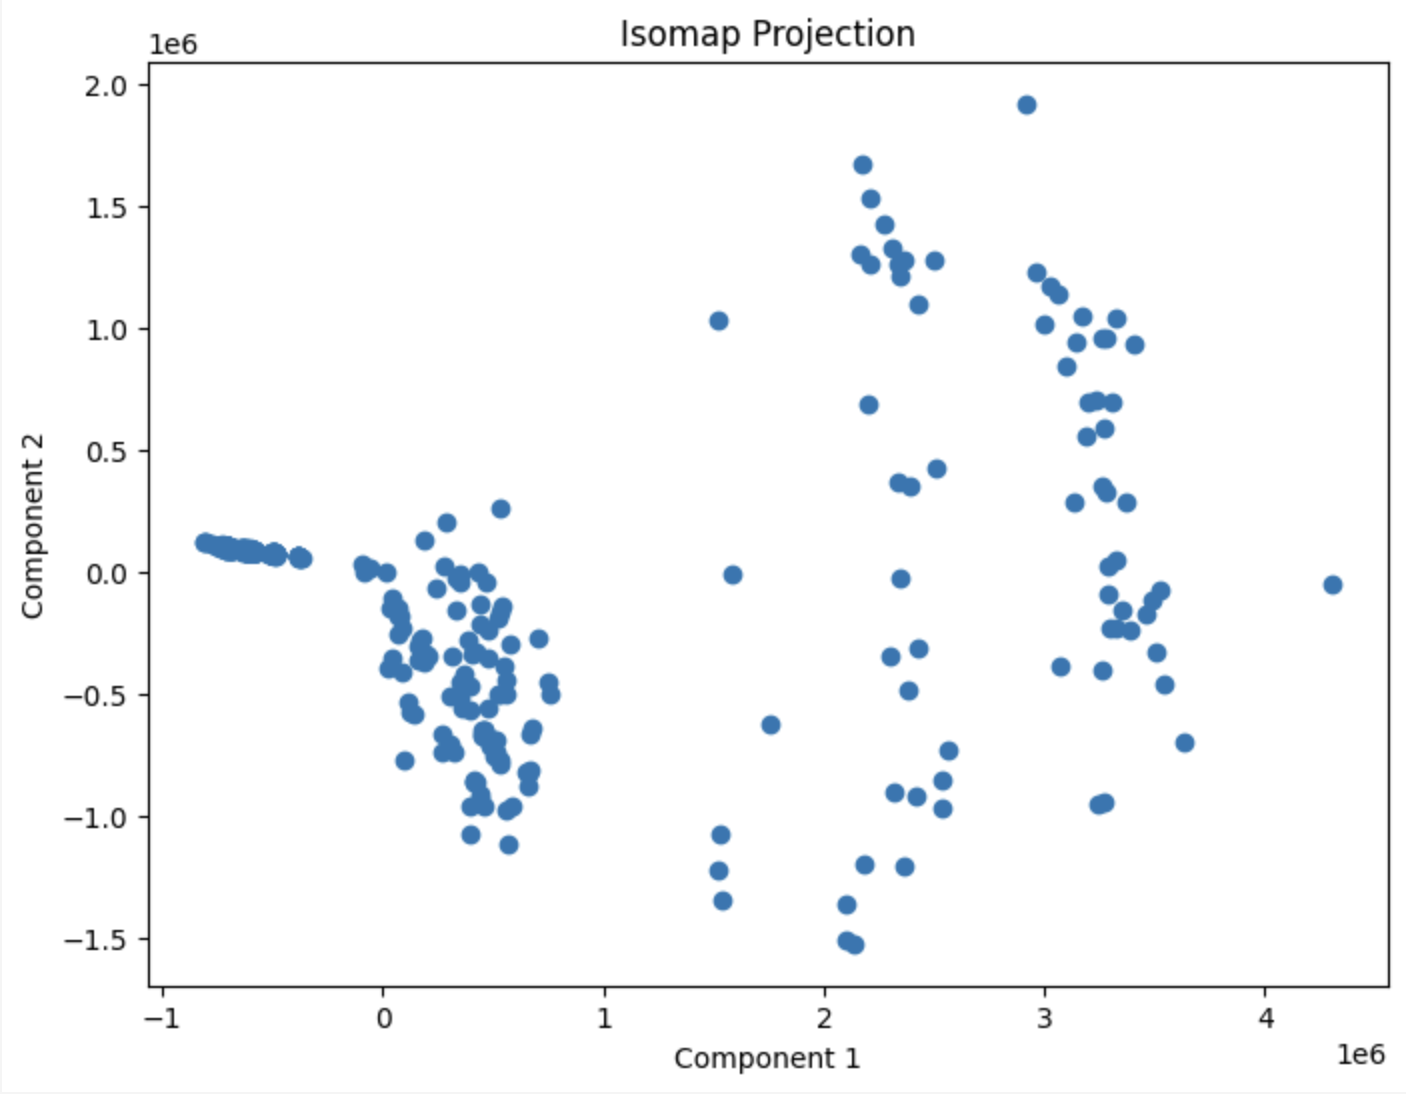
\includegraphics[width=\linewidth]{isomap_proj.png}
    \caption{Isomap при n\_components=2}
    \label{fig:isomap}
  \end{minipage}
\end{figure}

\begin{figure}[ht]
  \centering
  \begin{minipage}[b]{0.45\linewidth} 
    \centering
    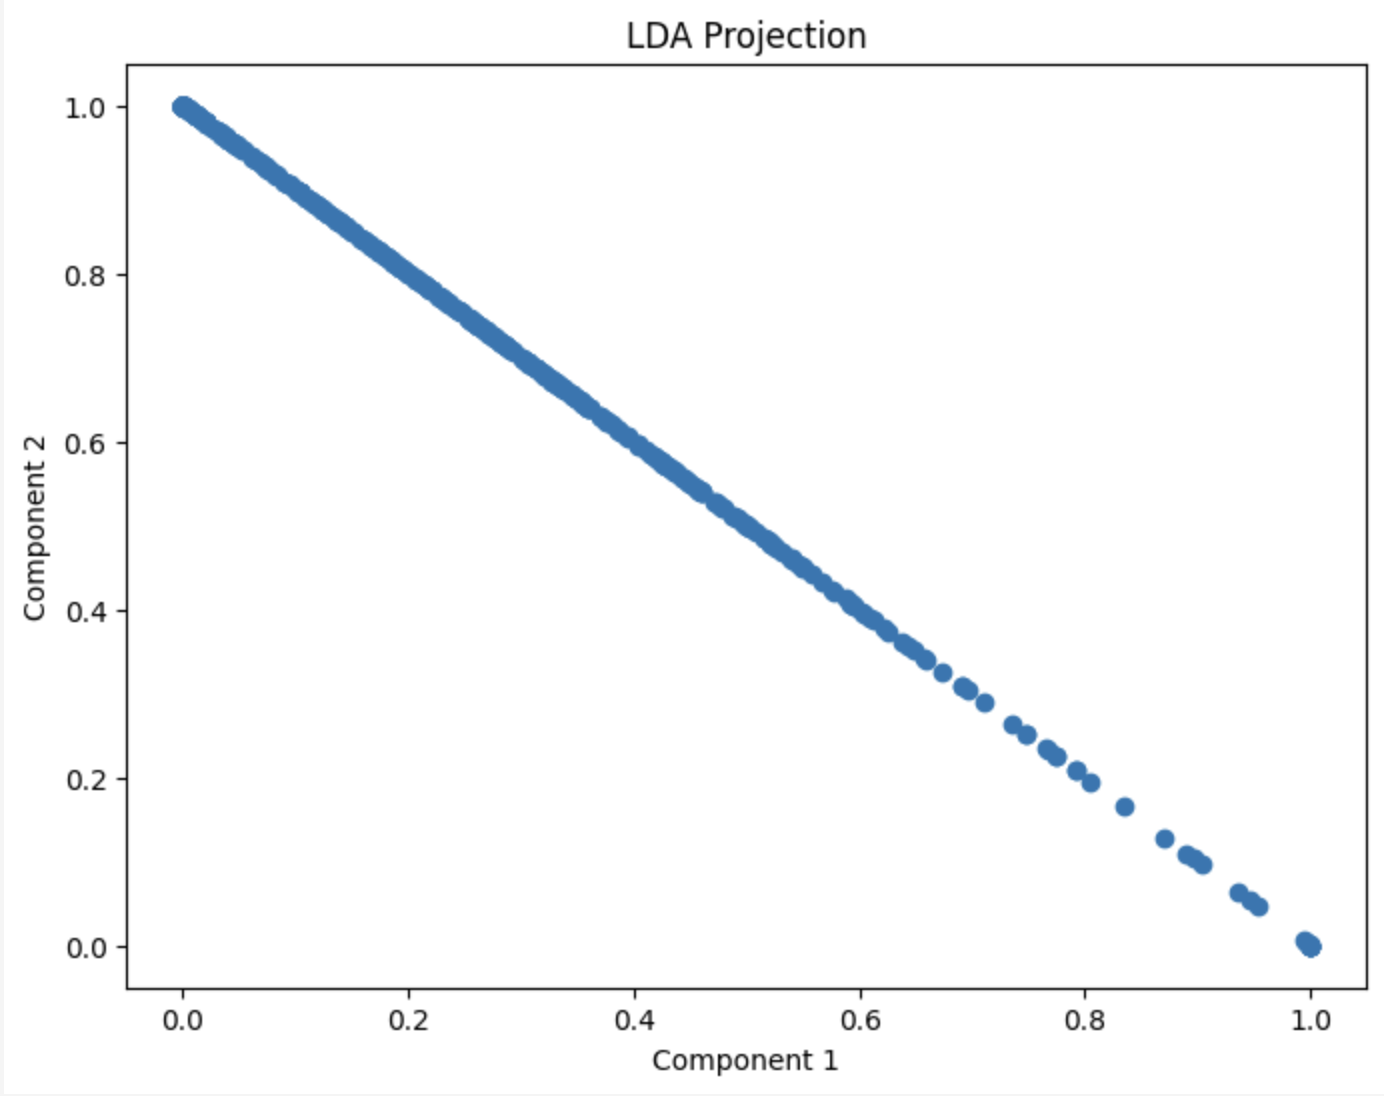
\includegraphics[width=\linewidth]{lda_proj.png}
    \caption{LDA при n\_components=2}
    \label{fig:lda}
  \end{minipage}
\end{figure}

Анализируя результаты применения различных методов понижения размерности (PCA, TSNE, Isomap, MDS, LDA, LLE, UMAP), можно выделить следующие ключевые недостатки:

\begin{itemize}
    \item При проецировании из высокоразмерного пространства в двумерное неизбежно теряется значительная часть геометрической информации, что критично для медицинских данных;
    
    \item Большинство методов не могут одновременно сохранить как локальные, так и глобальные свойства данных, что приводит к нерепрезентативным кластерам;
    
    \item Полученные проекции сложно интерпретировать с медицинской точки зрения, так как связь с исходными анатомическими структурами теряется.
\end{itemize}

При этом у этих методов есть недостатки с точки зрения дифференциальной геометрии, которые в том числе отражаются на качестве итогового разбиения на кластеры:

\begin{itemize}
    \item Стандартные методы не учитывают, что МРТ-данные часто лежат на искривленном многообразии с нетривиальной метрикой;
    
    \item Важные характеристики, например, секционная и скалярная кривизна, полностью теряются при понижении размерности;
    
    \item Расстояния между точками в проекции не соответствуют истинным геодезическим расстояниям на многообразии данных, следовательно, мы не можем правильно интерпретировать полученное разбиение на кластеры с медицинской (практической) точки зрения.
\end{itemize}

Итого, мы можем сделать вывод, что хоть и предложенные методы и являются популярными, но на практике не подходят для аналитики многомерных МРТ снимков. 

\section{Топологические методы анализа данных}

\subsection{Персистентные диаграммы}

Одним из ключевых инструментов в топологическом анализе данные являются персистентные диаграммы. Они позволяют количественно характеризовать многомерную топологическую структуру данных. В контексте анализа МРТ-изображений это означает, что они обеспечивают математически строгий подход к обнаружению и анализу значимых геометрических структур, например, они позволяют обнаружить компоненты связности, циклы и полости, которые могут отражать важные анатомические особенности и патологические изменения. 

Сначала обсудим теоретическое обоснование. Персистентные диаграммы основаны на концепции персистентных гомологий, которые отслеживают, как топологические особенности ``рождаются'' и ``умирают'' в процессе фильтрации данных. Зафиксируем размерность k. Теперь для каждой размерности k, где k = \{0, 1, 2, \dots\} зафиксируем k-мерные топологические особенности:

\begin{itemize}
    \item k = 0: компоненты связности (отдельные кластеры);
    
    \item k = 1: циклы или петли (одномерные ``дыры'');
    
    \item k = 2: полости (двумерные ``пустоты'').
\end{itemize}

Более формально, у нас есть облако точек $X \subset \mathbb{R}^d$ и параметр фильтрации $\epsilon$. Для них мы строим последовательность симплициальных комплексов $\{K_\epsilon\}_{\epsilon \geq 0}$, называемую фильтрацией. По мере увеличения $\epsilon$, мы отслеживаем, когда топологические особенности появляются и исчезают.

Если возвращаться к нашей задаче аналитики снимков МРТ, мы сначала должны преобразовать снимки в многомерные векторы, где каждый воксель или его характеристики становятся координатами в высокоразмерном пространстве. Далее для набора точек, представляющих МРТ-данные, рассчитывается матрица попарных расстояний. На основе матрицы расстояний строится последовательность симплициальных комплексов с возрастающим параметром $\epsilon$. 

\subsection{Алгоритм Ripser}

Для расчета матрицы расстояний мы будем использовать алгоритм Ripser [18]. Этот алгоритм является высокоэффективной реализацией для вычисления персистентных гомологий. В его основе лежит построение фильтрации комплекса Вьеториса-Рипса (Vietoris-Rips complex), где для множества точек $X \subset \mathbb{R}^d$ и параметра $\epsilon \geq 0$ комплекс $\text{Rips}_\epsilon(X)$ содержит симплекс $[v_0, v_1, \ldots, v_k]$ тогда и только тогда, когда $d(v_i, v_j) \leq 2\epsilon$ для всех пар вершин. Ключевое отличие алгоритма заключается в использовании когомологического подхода вместо гомологического, что позволяет избежать явного хранения всех симплексов. При редукции граничной матрицы $\partial$, представленной в виде матрицы $M$, алгоритм выявляет пары $(i, j)$, соответствующие рождению и смерти топологических особенностей, если $\text{low}(j) = i$. 

Важной оптимизацией является техника очистки (clearing), при которой если колонка $j$ соответствует положительно-градуированному симплексу с $\text{low}(j) = i$, то все последующие колонки $k > j$ с $\text{low}(k) = i$ можно пропустить, поскольку они не влияют на результат. С математической точки зрения, процесс вычисления персистентности представляет собой анализ изменений в гомологических группах 

    \begin{equation} H_*(K_\epsilon) = \frac{\text{ker} \ \partial_*}{\text{im} \ \partial_{*+1}} 
    \end{equation}
    при изменении параметра $\epsilon$, что позволяет формировать персистентные диаграммы, отражающие рождение и смерть топологических особенностей в данных.

\subsection{Визуализация персистентных диаграмм}

Итого, для каждой размерности k мы можем определить моменты ``рождения'' и ``смерти'' топологических особенностей. После этого для каждой точки $(b_i, d_i)$ на диаграмме соответствует топологической особенности, которая появилась при значении параметра $b_i$ и исчезла при значении $d_i$. Это означает, что персистентные диаграммы представляют собой двумерные графики, где горизонтальная ось соответствует моменту ``рождения'' топологической особенности, а вертикальная ось соответствует моменту ``смерти'' топологической особенности. Важно отметить, что диагональ $x = y$ представляет особенности с нулевой персистентностью (шум). Пример такого случая можно увидеть на рисунке ~\ref{fig:persistence_diagrams}.

\begin{figure}[ht]
  \centering
  \begin{minipage}[b]{0.9\linewidth} 
    \centering
    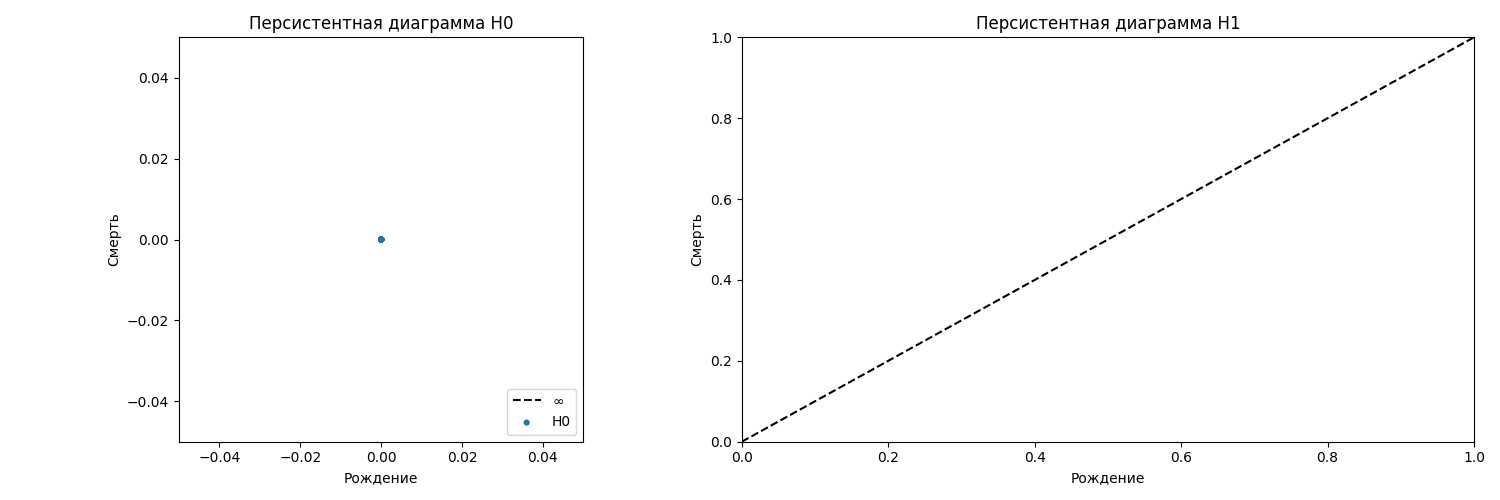
\includegraphics[width=\linewidth]{persistence_diagrams.png}
    \caption{Визуализация персистентных диаграмм, случай нулевой персистентности}
    \label{fig:persistence_diagrams}
  \end{minipage}
\end{figure}

При аналитики МРТ-снимков мы можем интерпретировать графики следующим образом: 

\begin{itemize}
    \item Диаграмма $H_0$ показывает, как отдельные компоненты данных объединяются при увеличении параметра фильтрации. С точки зрения МРТ это может отражать кластерную структуру интенсивностей в МРТ;
    
    \item Диаграмма $H_1$ выявляет циклические структуры, которые могут соответствовать анатомическим контурам или границам областей в мозге.
\end{itemize}

Таким образом, график $H_0$ из одной точки и имеющий вид диагонали график $H_1$ показывают, что изменений в строении мозга скорее всего нет. 

\subsection{Визуализация персистентных диаграмм с особенностями}

Построим персистентные диаграммы, но на данных с особенностями. Полученные диаграммы можно увидеть на рисунке ~\ref{fig:persistence_diagrams_with_anomaly}.

\begin{figure}[ht]
  \centering
  \begin{minipage}[b]{0.9\linewidth} 
    \centering
    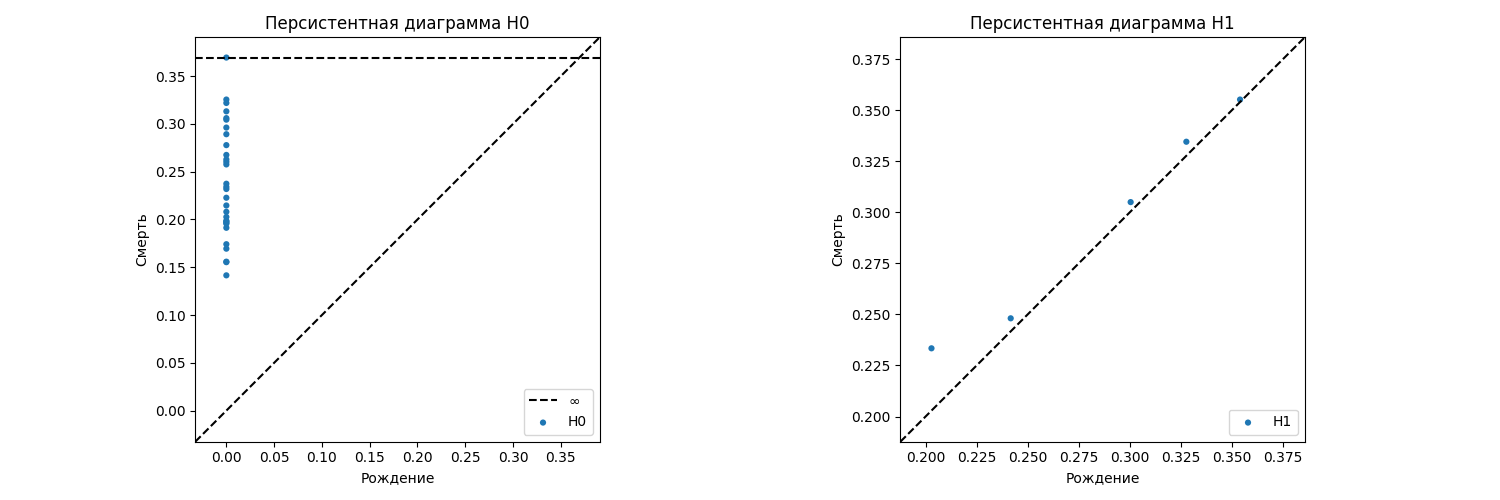
\includegraphics[width=\linewidth]{persistence_diagrams_with_anomaly.png}
    \caption{Визуализация персистентных диаграмм, случай с особенностями}
    \label{fig:persistence_diagrams_with_anomaly}
  \end{minipage}
\end{figure}

Заметим, что на данных графиках есть явные отличия от графиков для случая с нулевой персистентностью. Мы видим, что на графике $H_0$ уже не одна точка, а несколько, причем большинство точек расположены близко к оси рождения, что типично для компонентов связности. На графике $H_1$ точки вдоль диагонали означают малозначимые циклы. При этом особенность могла бы проявиться как точка значительно далеко от диагонали, показывая долгоживущий и значительный цикл. В данном примере такая точка имеет примерную координату (0.2, 0.23).

\section{Графы Риба в топологическом анализе МРТ-данных}

\subsection{Определение и концепция графов Риба}

Граф Риба (Reeb graph) [19] представляет собой топологическую структуру, которая упрощает представление многомерных данных путем кодирования глобальной структуры многообразия относительно некоторой функции фильтрации. В контексте нашей задачи это означает, что мы можем по многомерному МРТ-снимку построить сначала закодированное представление глобальной структуры, а далее использовать ее для анализа аномолий. 

Более формально, для топологического пространства $X$ и непрерывной функции $f: X \rightarrow \mathbb{R}$, граф Риба $\mathcal{R}_f(X)$ определяется как фактор-пространство $X/{\sim}$, где отношение эквивалентности $\sim$ задается следующим образом: $x_1 \sim x_2$ тогда и только тогда, когда $f(x_1) = f(x_2)$ и точки $x_1$ и $x_2$ принадлежат одной компоненте связности множества $f^{-1}(f(x_1))$.

В контексте анализа МРТ-данных это означает, что графы Риба обеспечивают эффективное представление глобальной топологической структуры данных. В теории они могут выделить важные особенности и устранить избыточную информацию. Данное качество как раз исправляет один из явных недостатков методов понижения размерности, так как они тоже пытались удалить избыточную информацию, но вместе с ней в том числе удаляли и полезные данные. 

Итого, графы Риба могут помочь нам визуализировать сложные многомерные структуры в виде одномерных графов и в последствии облегчить их интерпретацию и анализ.

\subsection{Построение графов Риба для МРТ-данных}

Подход по применению графов Риба для аналитики снимков МРТ был сделан в статье [20], но тогда авторы не смогли прийти к хорошему решению из-за формата снимков, в котором они имеют небольшую размерность. В нашем же подходе мы работаем с данными большой размерности, а значит в теории можем получить хорошую обработку. 

Перейдем к процессу построения графа Риба для МРТ-данных. Сначала мы должны выбрать функции фильтрации. Для многомерных МРТ-данных в качестве функции фильтрации часто используется первая главная компонента, полученная с помощью метода главных компонент (PCA), что в итоге обеспечивает направление наибольшей дисперсии в данных:
    \begin{equation}
        f(x) = \langle x, v_1 \rangle
    \end{equation}
    где $v_1$ — первый собственный вектор ковариационной матрицы данных.
    
Далее мы должны сделать разбиение диапазона значений функции. Мы будем разбивать диапазон значений функции $f$ на $m$ равных интервалов $[a_i, a_{i+1}]$, где $i \in \{0, 1, \ldots, m-1\}$. Итого, разбиение имеет вид:
    \begin{equation}
        a_i = f_{min} + i \cdot \frac{f_{max} - f_{min}}{m}
    \end{equation}
    
Следующим шагом является определение компонент связности. Для каждого интервала $[a_i, a_{i+1}]$ мы найдем все точки $x \in X$, для которых $f(x) \in [a_i, a_{i+1})$. Далее мы сможем определить компоненты связности этого множества. Каждая компонента связности становится вершиной графа Риба. Две вершины соединяются ребром, если соответствующие компоненты связности в соседних интервалах имеют общие точки.

\subsection{Алгоритмическая реализация}

Перейдем к реализации построения графа Риба. На вход мы принимаем наши данные МРТ-снимков $X \in \mathbb{R}^{n \times d}$, функцию фильтрации $f: X \rightarrow \mathbb{R}$, а так же число интервалов $m$. На выходе мы хотим получить граф $G = (V, E)$.

Сначала мы должны вычислить значения функции $f(x)$ для всех точек $x \in X$ и найти минимальное и максимальное значения $f_{min}$ и $f_{max}$. Далее, зная эти значения, мы можем разбить интервал $[f_{min}, f_{max}]$ на $m$ равных частей с границами $\{a_0, a_1, \ldots, a_m\}$.


Теперь перейдем к самому алгоритму. Создадим пустой граф $G = (V, E)$ и выполним следующий цикл:

\begin{algorithmic}
\For{$i = 1$ \textbf{до} $m$}
    \State Найти все точки $X_i = \{x \in X : f(x) \in [a_{i-1}, a_i]\}$
    \State Определить компоненты связности $\{C_{i,j}\}$ множества $X_i$
    \State Добавить в $V$ вершину для каждой компоненты $C_{i,j}$
\EndFor

\For{$i = 1$ \textbf{до} $m-1$}
    \For{каждой пары компонент $C_{i,j}$ и $C_{i+1,k}$}
        \If{$C_{i,j} \cap C_{i+1,k} \neq \emptyset$}
            \State Добавить ребро между соответствующими вершинами в $G$
        \EndIf
    \EndFor
\EndFor
\end{algorithmic}

Итого, на выходе мы получим граф Риба на основе векторного представления МРТ-снимка.

\subsection{Применение графов Риба в анализе МРТ-данных}

На предыдущем шаге мы получили граф Риба. Теперь рассмотрим, как мы можем применить его на практике для анализа МРТ-снимков. Выше мы описали, что графы Риба позволяют обнаруживать и анализировать глобальные топологические особенности в МРТ-данных. В том числе различные ветви графа Риба могут соответствовать различным анатомическим структурам в МРТ-снимках, что позволяет проводить их автоматическую сегментацию.

В нашей задаче мы хотим научитьcя эффективно находить особенности в данные. Аномальные структуры в графе Риба могут указывать на наличие патологий в МРТ-снимках, например,  опухоли или другие морфологические изменения. Таким образом, графы Риба могут использоваться как основа для классификации и сравнения МРТ-снимков путем вычисления расстояний между графами.

Для эффективной визуализации графов Риба в нашем анализе МРТ-данных мы использовали несколько техник. Во-первых, мы применили цветовое кодирование, где вершины графа окрашивались в соответствии со значением функции фильтрации. Это позволило визуально отслеживать изменения функции. Во-вторых, размер каждой вершины был пропорционален количеству точек в соответствующей компоненте связности, что показывало относительную важность каждой компоненты. Наконец, пространственное расположение графа визуализировалось так, чтобы вертикальная координата вершины соответствовала значению функции фильтрации, что облегчало восприятие структуры данных.

\subsection{Анализ полученного графа}

В результате описанных выше действий был получен граф, который можно увидеть на рисунке ~\ref{fig:reeb_graph}.

\begin{figure}[ht]
  \centering
  \begin{minipage}[b]{0.9\linewidth} 
    \centering
    
\includegraphics[width=\linewidth]{reeb_graph.png}
    \caption{Визуализация графа Риба}
    \label{fig:reeb_graph}
  \end{minipage}
\end{figure}

Теперь нам нужно интерпретировать полученный граф. Мы знаем, что граф Риба представляет собой упрощённое представление множества уровней функции Морса, где каждая точка графа соответствует компоненте связности уровня данной функции.

Мы видим, что наш граф имеет иерархическую структуру, где вершины находятся на разных уровнях. Это может указывать на изменения топологии при изменении значения функции. Узлы графа, например, точки interval\_5, interval\_6, и interval\_7, могут представлять критические точки, которые связаны с важными изменениями в топологической структуре. Наш граф не содержит циклов, что характерно для представления изменения однопараметрической величины, как функция высоты над поверхностью, но узел interval\_2 ведет к последовательности других, что может указывать на область с постепенным развитием топологии.

\section{Сбор единого инструмента для анализа МРТ-снимков}

\subsection{Архитектура фреймворка}

В разделах выше мы описали построение персистентных диаграмм и графов Риба. Мы хотим, чтобы наш итоговый фреймворк мог принять данные МРТ, преобразовать их в нужный формат и найти особенности. Причем нам важен не только сам вердикт, но и последующее преобразование исходных данных назад в 2D-снимок с выделенными особенностями. Данное преобразование нужно не только для удобной интерпретации данных, но и для помощи врачу в определении диагноза.

Для дальнейшей аналитики снимков мы можем объединить метод персистентных диаграмм и графы Риба. Причем нам будет полезно создать снимки в разных срезах. Так как мы работает с многомерным пространством – сканом МРТ, мы можем сами выбрать срезы, которые нам были бы интересны. В качестве срезов для изображений мы выбрали аксиальный (горизонтальный срез, который делит тело на верхнюю и нижнюю части), сагиттальный (вертикальный срез, проходящий спереди назад, делит тело на левую и правую части) и корональный (вертикальный срез, который делит тело на переднюю и заднюю части) срезы. 

\subsection{Построение изображений срезов}

Перейдем к построению изображений срезов. Аксиальный срез получается путём вырезания горизонтального слоя из середины изображения вдоль оси Z, для сагиттального среза мы будем брать вертикальный слой из середины вдоль оси Y, а для коронального среза мы выделим вертикальный слой из середины вдоль оси X. Для построения графиков мы будем использовать библиотеку Matplotlib\footnote{Библиотека доступна по ссылке: \url{https://matplotlib.org}, дата обр. 08.04.2025}, в итоге мы сможем получить представление о выбранных плоскостях. Полученные изображения можно увидеть на рисунке ~\ref{fig:mri_visualization}.

\begin{figure}[ht]
  \centering
  \begin{minipage}[b]{0.9\linewidth} 
    \centering
    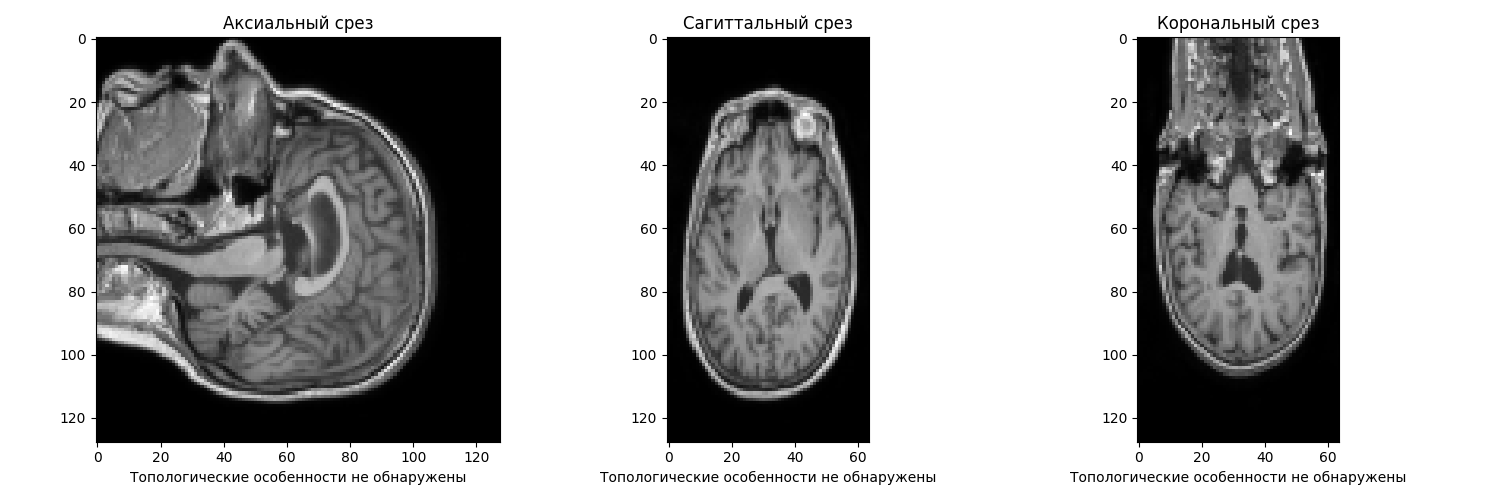
\includegraphics[width=\linewidth]{mri_visualization.png}
    \caption{Визуализация срезов МРТ-снимка без особенностей}
    \label{fig:mri_visualization}
  \end{minipage}
\end{figure}

\subsection{Построение изображений срезов c особенностями}

Теперь мы должны добавить в код определение особенностей. Причем для интерпретации результатов нам необходимо, чтобы на срезах мы видели области, которые имеют топологические особенности. Итоговый код должен уметь выявлять топологические особенности с помощью персистентных диаграмм и графов Риба, которые мы описывали в предыдущих секциях. Мы знаем, что персистентные диаграммы отображают жизненный цикл топологических свойств данных и точки на диаграмме, расположенные далеко от диагонали, указывают на значительные топологические особенности. Значит код может использовать эти диаграммы, чтобы идентифицировать и интерпретировать длительные и значимые топологические структуры, следовательно, находить особенности. 

Для создания графа Риба применяется функция фильтрации. В качестве этой функции  мы будем использовать первую главная компонента (PCA), чтобы выделить важные направления изменений в данных. Эксперименты показали, что с помощью этой функции можно получить хорошое определение особенностей. Далее процесс похож на построение графов Риба, который был описан выше: диапазон значений функции фильтрации делится на равные интервалы, где каждый интервал соответствует узлу в графе. В каждом узле хранится информация об уровне, размере (число точек в интервале) и среднем значении фильтрации. Далее узлы соединяются рёбрами. Они отображают изменения структуры между интервалами и демонстрируют, как данные трансформируются при изменении значений функции фильтрации.

Дополнительно мы используем персистентные диаграммы. Если все диаграммы пусты, мы будем возвращать нулевой вектор признаков, что означает отсутствие особенностей. В противном случае для каждой диаграммы будем вычислять стойкости (разность между смертью и рождением топологических особенностей) и будем извлекать из стойкостей  статистические данные: количество, сумма, среднее, стандартное отклонение, максимум и 75-й процентиль. Далее с помощью библиотки persim\footnote{Библиотека доступна по ссылке: \url{https://persim.scikit-tda.org/en/latest}, дата обр. 08.04.2025} для каждой диаграммы создаются изображения, которые отображают распределение стойкостей. Если точек в диаграмме нет, будет строиться нулевое изображение. После такого процесса все вычисленные признаки и изображения вытягиваются в одномерные массивы и конкатенируются в один вектор. Следующим шагом мы можем выбрать только те особенности, персистентность которых превышает пороговое значение, и выделить их на изображении. В итоге мы получаем вердикт, что в снимке есть особенность, а так же изображение, на котором эта особенность выделена. Пример изображения можно увидеть на рисунке ~\ref{fig:mri_comparison_with_features}.

\begin{figure}[ht]
  \centering
  \begin{minipage}[b]{0.9\linewidth} 
    \centering
    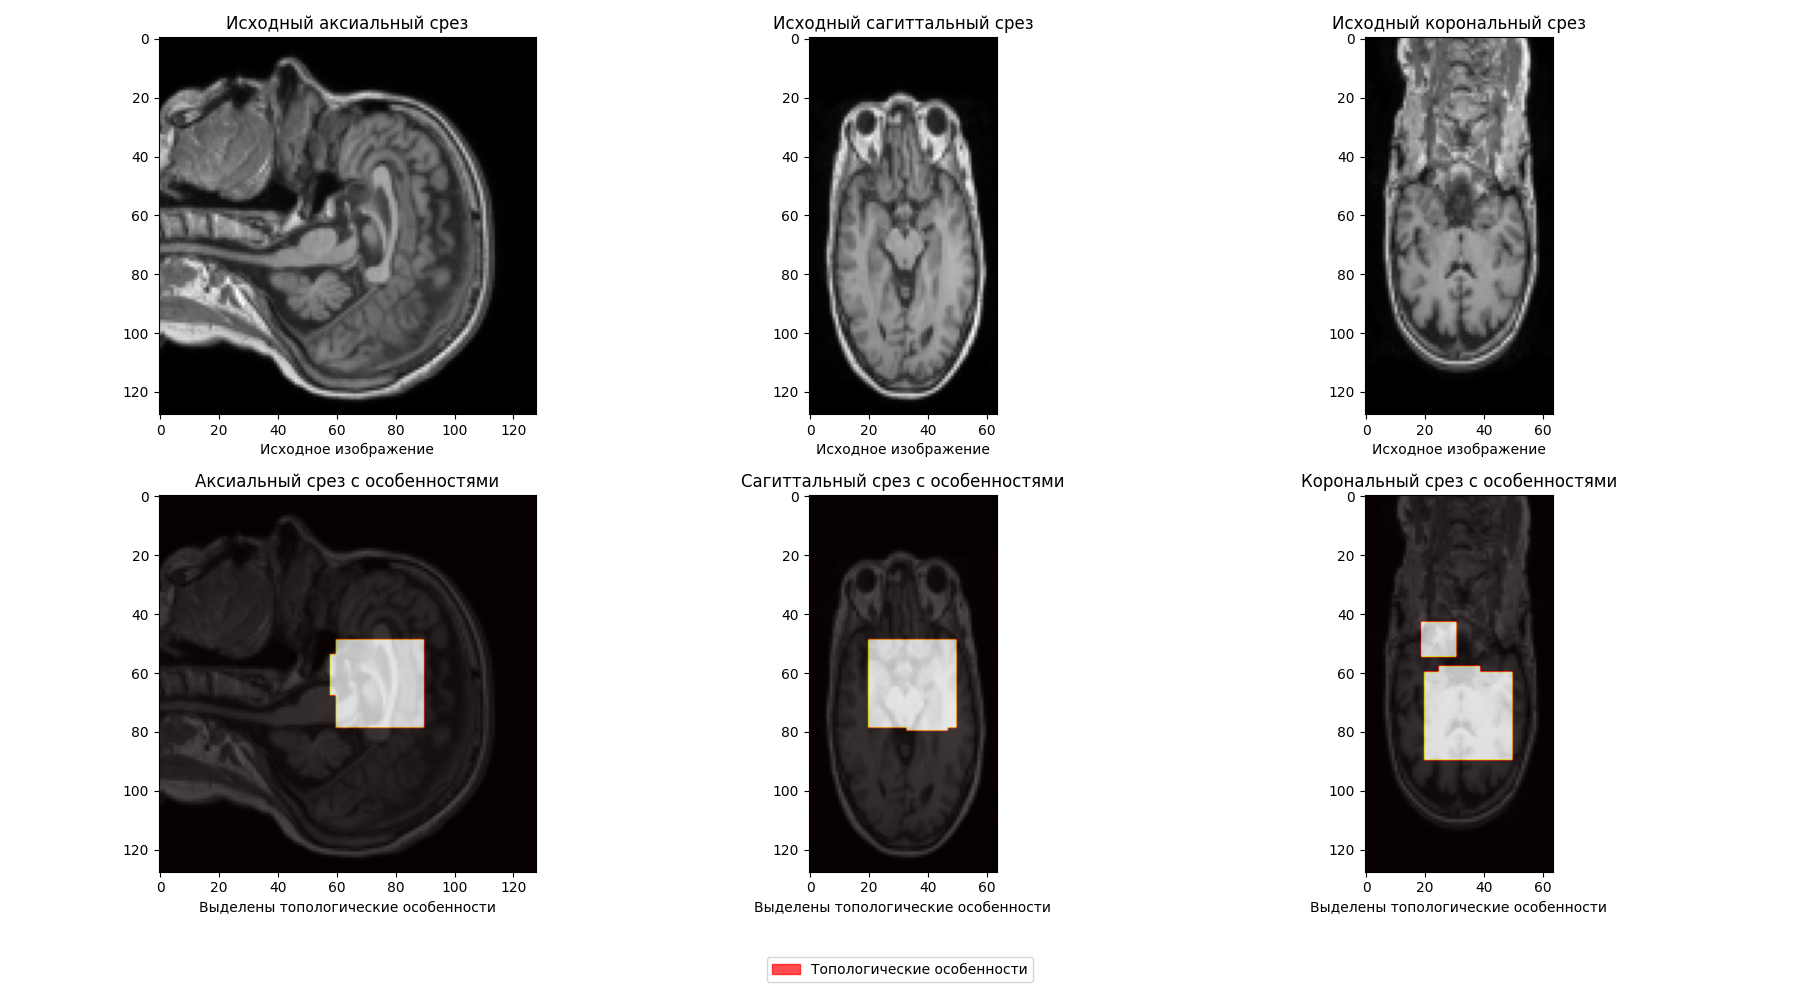
\includegraphics[width=\linewidth]{mri_comparison_with_features.png}
    \caption{Визуализация срезов МРТ-снимка c особенностями}
    \label{fig:mri_comparison_with_features}
  \end{minipage}
\end{figure}

\subsection{Замер качества выделения особенностей}

Итого, на данном этапе работы у нас появился инструмент, который объединяет персистентные диаграммы и графы Риба и определяет особенность в пространстве точек. Теперь нам необходимо замерить качество полученного инструмента. В качестве метрик будем использовать ROC–AUC и PR–AUC [22]. Замерять эффективность фреймворка будем следующим образом: 

\begin{enumerate}
    \item Создадим копию исходных МРТ–данных. Далее в эту копию искусственно добавим особенности (в  примерно 30\% образцов). Особенности будут представлять собой точки с измененной интенсивностью в случайных областях изображения;

    \item Следующим шагом для каждого образца (как нормального, так и с особенностями) будем вычислять диаграммы персистентности, причем код будет пробовать разные метрики (евклидова, корреляция, косинусная) для обнаружения более выраженных топологических особенностей. Итого, на этом шаге персистентная гомология измеряет, как меняются компоненты связности (H0) и циклы (H1) при изменении порога фильтрации;

    \item Если в результате предыдущего шага были найдены особенности H1 (циклы), будем использовать среднюю продолжительность жизни этих особенностей как показатель аномальности. В противном случае, если особенности H1 не найдены, будем использовать особенности H0 (компоненты связности). Для H0 применим стандартное отклонение времени жизни конечных компонент или количество компонент как запасной вариант. Если значения оценки велики, они указывают на потенциальные особенности;

    \item Итого, мы получили некоторые оценки, которые мы можем нормировать (привести к диапазону [0; 1]) и вычислить значения метрик ROC–AUC и PR–AUC. 
\end{enumerate}

\subsection{Аналитика получившихся метрик}

Итого, мы получили графики, демонстрирующие качество обнаружения особенностей. Эти графики дают представление о качестве модели, их можно увидеть на рисунке ~\ref{fig:anomaly_detection}.

\begin{figure}[ht]
  \centering
  \begin{minipage}[b]{0.9\linewidth} 
    \centering
    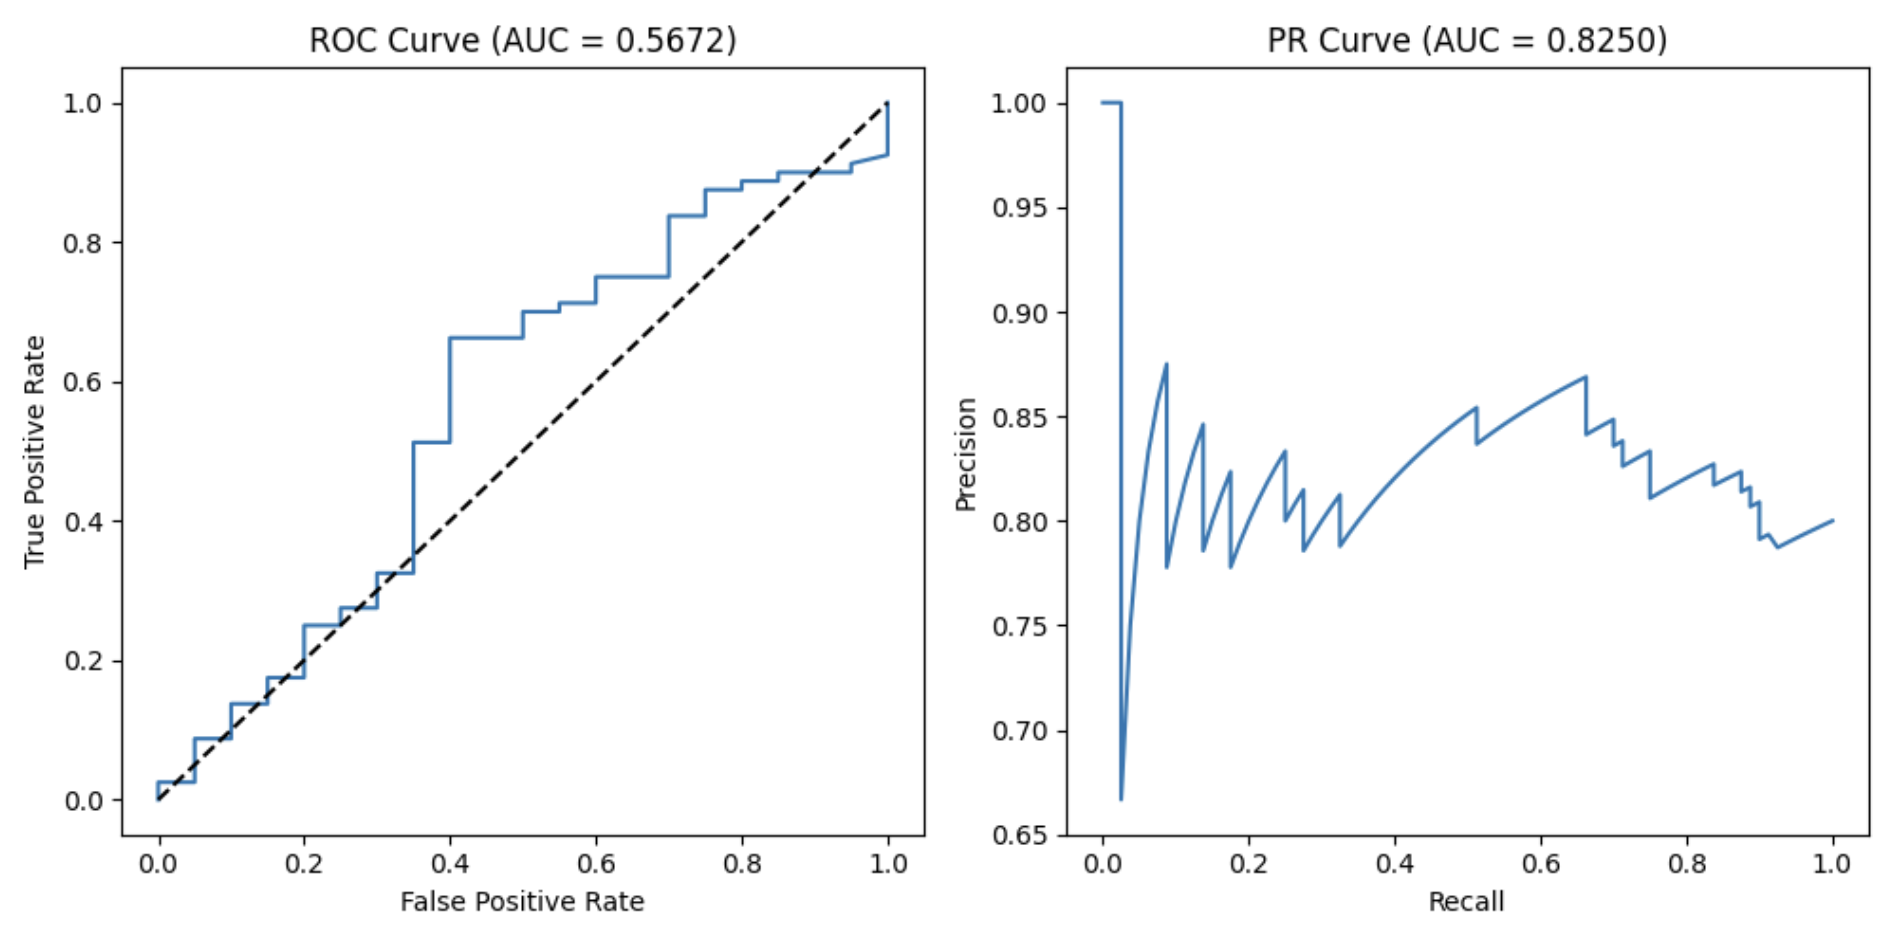
\includegraphics[width=\linewidth]{anomaly_detection.png}
    \caption{ROC–AUC и PR–AUC определения особенностей}
    \label{fig:anomaly_detection}
  \end{minipage}
\end{figure}

На первом (левом) графике изображена ROC-кривая, она показывает соотношение между True Positive Rate (чувствительность) и False Positive Rate (1-специфичность) при разных порогах. Известно, что чем выше кривая над диагональю, тем лучше алгоритм, можем заметить, что наш алгоритм немного лучше случайного угадывания. На втором (правом) графике изображена PR-кривая, которая показывает соотношение между точностью (Precision) и полнотой (Recall) при разных порогах. Данная метрика особенно полезна при несбалансированных данных, которыми являются наши снимки, так как по умолчанию мы подразумеванием, что количество особенностей и обычных снимков должно сильно различаться. Итого, на PR-кривой видно, что наш метод имеет высокую точностью обнаружения особенностей.

\section{Методы дифференциальной геометрии}

\subsection{Анализ кривизны многообразия данных}

Как мы могли увидеть в предыдущем разделе, инструмент, который объединяет персистентные диаграммы и графы Риба, справляется с определением особенностей в МРТ-снимках, но нуждается в улучшениях из-за небольшого значения метрики ROC-AUC. Для улучшения метрик мы будем использовать методы дифференциальной геометрии. Начнем с анализа кривизны многообразия данных [23]. При анализе сложных многомерных данных мы часто сталкиваемся с интуитивным пониманием, что данные лежат не просто в пространстве всех возможных значений, а образуют некоторую структуру -- многообразие. Чтобы формализовать это понимание, обратимся к аппарату дифференциальной геометрии, который позволяет описывать локальные и глобальные свойства таких многообразий. Анализ кривизны многообразия данных основан на предположении, что набор данных лежит на некотором многообразии, вложенном в пространство более высокой размерности. Кривизна этого многообразия может служить индикатором необычных структур или особенностей.

Представим наши данные как точки $n$-мерного многообразия $M$, вложенного в объемлющее пространство $\mathbb{R}^d$, где $d > n$. Для понимания геометрии многообразия ключевым понятием выступает метрический тензор \begin{equation}g_{ij}(p) = \langle \partial_i, \partial_j \rangle\end{equation} где $\partial_i = \frac{\partial}{\partial x^i}$ и $\partial_j = \frac{\partial}{\partial x^j}$ -- базисные векторы касательного пространства $T_p M$ в точке $p$. Метрический тензор позволяет нам определить, как измеряются расстояния и углы на нашем многообразии, что критично для понимания структуры данных.

Однако, чтобы говорить о кривизне, нам необходимо понять, как изменяются касательные векторы при перемещении по многообразию. Эту роль выполняет связность $\nabla$, определяющая способ параллельного переноса векторных полей. Математически это выражается через ковариантную производную $\nabla_X Y$, которая в локальных координатах записывается как \begin{equation}\nabla_i \partial_j = \Gamma^k_{ij} \partial_k\end{equation} Здесь появляются символы Кристоффеля $\Gamma^k_{ij}$ [24], связывающие геометрию с алгеброй через соотношение \begin{equation}\Gamma^k_{ij} = \frac{1}{2} g^{kl} \left( \frac{\partial g_{jl}}{\partial x^i} + \frac{\partial g_{il}}{\partial x^j} - \frac{\partial g_{ij}}{\partial x^l} \right)\end{equation}

Наиболее фундаментальной характеристикой многообразия, отражающей его отклонение от плоского пространства, является тензор кривизны Римана [25] \begin{equation}R(X, Y)Z = \nabla_X \nabla_Y Z - \nabla_Y \nabla_X Z - \nabla_{[X, Y]} Z\end{equation} В координатной форме этот тензор выражается через производные и произведения символов Кристоффеля: \begin{equation}R^m_{ijk} = \frac{\partial \Gamma^m_{jk}}{\partial x^i} - \frac{\partial \Gamma^m_{ik}}{\partial x^j} + \Gamma^n_{jk}\Gamma^m_{in} - \Gamma^n_{ik}\Gamma^m_{jn}\end{equation} с понижением индекса через метрику: \begin{equation}R_{ijkl} = g_{lm} R^m_{ijk}\end{equation}

Полный тензор кривизны содержит исчерпывающую информацию, но его сложно визуализировать и интерпретировать. Поэтому введем более наглядные характеристики. Секционная кривизна $K(X,Y)$ позволяет ``изолировать'' кривизну в конкретном двумерном направлении, задаваемом векторами $X$ и $Y$: \begin{equation}K(X,Y) = \frac{R(X,Y,Y,X)}{\|X\|^2\|Y\|^2 - \langle X,Y \rangle^2}\end{equation} Для ортонормированного базиса эта формула принимает вид: \begin{equation}K(e_i, e_j) = R_{ijji}\end{equation}

Когда мы работаем с многомерными данными, удобнее рассматривать усредненные характеристики кривизны по различным направлениям. Тензор Риччи [26] \begin{equation}\text{Ric}_{ij} = R^k_{ikj} = g^{kl}R_{kilj}\end{equation} возникает как свертка тензора Римана и геометрически отражает, насколько объем, заключенный в малой окрестности точки многообразия, отличается от соответствующего евклидова объема. Скалярная кривизна \begin{equation}R = g^{ij}\text{Ric}_{ij}\end{equation} ещё дальше продвигает это усреднение, превращая тензор кривизны в единое число, характеризующее ``изогнутость'' многообразия в данной точке. В итоге мы получаем инструмент, аналогичный тому, как гауссова кривизна описывает изогнутость поверхности.

Перенося эти абстрактные математические концепции в практическую плоскость анализа данных, мы сталкиваемся с задачей оценки кривизны для облака точек $\{x_1, x_2, \ldots, x_N\} \subset \mathbb{R}^d$. Здесь мы не имеем аналитического описания многообразия, а можем лишь аппроксимировать его локальные свойства. Один из подходов основан на анализе собственных значений локальной ковариационной матрицы: \begin{equation}C(x_i) = 1 - \frac{\lambda_{\min}}{\lambda_{\max}}\end{equation} где отношение минимального к максимальному собственному значению отражает ``сплющенность'' многообразия в данной точке. Альтернативный подход использует ошибку реконструкции: \begin{equation}E(x_i) = \frac{1}{k} \sum_{j \in \mathcal{N}_k(i)} \|x_j - \hat{x}_j\|^2\end{equation} Данный подход измеряет, насколько соседние точки отклоняются от касательной плоскости.

Итого, аномальные точки часто создают области с необычно высокой кривизной, поскольку они нарушают гладкую структуру основного многообразия данных. Объединив информацию о кривизне с топологическими методами, мы получаем инструмент, с помощью которого мы можем эффективно выявлять скрытые закономерности и выбросы.

\subsection{Применение кривизны многообразия данных для нахождения особенностей в МРТ-снимках}

Перейдем к реализации описанных выше методов и применению их на практике на МРТ-снимках с особенностями. Для простоты начнем с синтетических данных с заданным количеством кластеров, а далее применим полученный метод на пространстве точек, полученном в результате МРТ.

Сгенерируем данные следующим образом: создадим $n$-мерное многообразие, состоящее из $\text{n\_clusters}$ сферических компонент, расположенных в $\text{n\_features}$-мерном пространстве. С точки зрения дифференциальной геометрии, эти компоненты могут быть аппроксимированы как области с малой внутренней кривизной (близкие к евклидовым), но общее многообразие имеет сложную топологию, определяемую расположением компонент относительно друг друга. На синтетических данных будем находить особенности следующим образом: 

\begin{enumerate}
    \item Для каждой точки $x_i$ найдем $k$ ее соседей. Далее центрируем их, применяем SVD разложение $X_i = USV^T$ и оцениванием кривизну;

    \item Следующим шагом для каждой точки $x_i$ и её соседей аппроксимируем касательное пространство с помощью метода PCA, проецируем соседей на это пространство и обратно и в конце измеряем ошибку реконструкции;

    \item В конечном итоге финальная оценка аномальности сочетает кривизну и ошибку реконструкции. Далее по этой оценке и порогу мы можем определить принадлежность точки к аномалии.
\end{enumerate}

Итого, результаты работы метода на синтетических данных можно увидеть на рисунке ~\ref{fig:curvature_anomaly_detection}.

\begin{figure}[ht]
  \centering
  \begin{minipage}[b]{0.9\linewidth} 
    \centering
    
\includegraphics[width=\linewidth]{curvature_anomaly_detection.png}
    \caption{Результат работы метода, анализирующего кривизну многообразия данных}
    \label{fig:curvature_anomaly_detection}
  \end{minipage}
\end{figure}

Можем заметить, что у нас немного уменьшилось значение метрики PR–AUC (было 0.8250, стало 0.7750), но зато значимо увеличилось значение метрики ROC-AUC (было 0.5672, стало 0.9208), то есть данный метод показывает лучшие результаты по сравнению с топологическими методами и потенциально может показать лучшие результаты на МРТ-данных. 

Здесь не стоит забывать, что мы сравнивали значения метрик на идейно разных датасетах, поэтому следующим шагом необходимо замерить значения ROC-AUC и PR–AUC на данных с особенностями в результатах МРТ. Аналогично разделу 7.4 искусственно добавим особенности в МРТ-данные и попробуем с помощью анализа кривизны определить особенности (аналогично берем долю особенностей 30\% и те же самые МРТ-снимки). На данных, приближенных к настоящим, мы получаем значение ROC-AUC = 0.7943, PR-AUC = 0.7251. Заметим, что эти результаты лучше, чем результаты обнаружения особенностей топологическими методами. Графики метрик можно увидеть на рисунке ~\ref{fig:mri_curvature_performance}.

\begin{figure}[ht]
  \centering
  \begin{minipage}[b]{0.9\linewidth} 
    \centering
    
\includegraphics[width=\linewidth]{mri_curvature_performance.png}
    \caption{Результат работы метода, анализирующего кривизну многообразия данных (МРТ-данные)}
    \label{fig:mri_curvature_performance}
  \end{minipage}
\end{figure} 

\subsection{Метод расслоенных пространств (Fiber Bundles)}

Перейдем к методу расслоенных пространств (Fiber Bundles) [27], еще одному методу дифференциальной геометрии, и попробуем использовать его для нахождения особенностей. Сначала введем несколько определений:

\begin{itemize}
\item Расслоенное пространство (или расслоение) представляет собой четверку $(E, \pi, B, F)$, где $E$ — полное пространство расслоения, $B$ — база расслоения, $F$ — типичный слой, $\pi: E \to B$ — непрерывная сюръекция, называемая проекцией;

\item При этом для каждой точки $x \in B$ существует окрестность $U \subset B$, содержащая $x$, такая что $\pi^{-1}(U) \cong U \times F$, где изоморфизм сохраняет структуру слоев. Для каждой точки $x \in B$ множество $\pi^{-1}(x) \subset E$ называется слоем над точкой $x$ и обозначается $F_x$. Каждый слой $F_x$ гомеоморфен типичному слою $F$;

\item Сечением расслоения $(E, \pi, B, F)$ называется отображение $s: B \to E$, такое что $\pi \circ s = \text{id}_B$. Сечения моделируют поведение ``нормальных'' данных. Связность в расслоении — структура, позволяющая определить, как элементы слоев изменяются при перемещении по базе. Связность определяется распределением горизонтальных подпространств $H_p \subset T_p E$. Форма кривизны связности $\omega$ — это $\mathfrak{g}$-значная 2-форма, определяемая формулой:
\begin{equation}
\Omega = d\omega + \frac{1}{2}[\omega, \omega]
\end{equation}
Кривизна измеряет, насколько локальная структура данных отклоняется от плоской;

\item Параллельный перенос — перенос элементов слоя вдоль пути на базе, сохраняющий горизонтальность. Математически, для пути $\gamma: [0,1] \to B$, параллельный перенос — это изоморфизм $P_\gamma: \pi^{-1}(\gamma(0)) \to \pi^{-1}(\gamma(1))$. Голономия — мера изменения при параллельном переносе по замкнутому пути. Для нормальных данных голономия должна быть малой. Количественно для замкнутого пути $\gamma$ голономия выражается как отклонение $P_\gamma$ от тождественного отображения.

\end{itemize}

\subsection{Применение метода расслоенных пространств для поиска особенностей}

Теперь рассмотрим, как можно использовать эту теорию для поиска особенностей в данных. При обнаружении особенности мы рассматриваем данные как:
\begin{itemize}
    \item База $B$ — низкоразмерное многообразие, на котором лежат нормальные образцы;
    \item Слои $F_x$ — представляют локальные отклонения от многообразия;
    \item Полное пространство $E$ — все пространство данных.
\end{itemize}

Особенности часто вызывают локальные искажения многообразия данных, что проявляется как высокая кривизна. Локальную кривизну в точке $x$ можно оценить через отношение собственных значений:
\begin{equation}
\kappa(x) = 1 - \frac{\lambda_{\min}}{\lambda_{\max}}
\end{equation}
где $\lambda_{\min}$ и $\lambda_{\max}$ — минимальное и максимальное ненулевые собственные значения локальной ковариационной матрицы. Для особенностей характерна большая голономия, когда параллельный перенос по замкнутому пути не возвращает элемент в исходное положение. Количественно голономию для точки $x$ можно выразить как:
\begin{equation}
\text{Hol}(x) = \|I - P_{\gamma}\|_F
\end{equation}
где $P_{\gamma}$ — матрица параллельного переноса по замкнутому пути $\gamma$, а $\|\cdot\|_F$ — норма Фробениуса. Особенности нарушают гладкость сечений, что можно измерить через:
\begin{equation}
\text{Irr}(x) = \left\|\nabla s(x) - \frac{1}{|N(x)|}\sum_{y \in N(x)}\nabla s(y)\right\|
\end{equation}
где $N(x)$ — окрестность точки $x$, а $\nabla s$ — градиент сечения. Это означает, что на практике нерегулярность можно оценить через ошибку реконструкции:
\begin{equation}
\text{Err}(x) = \frac{1}{|N(x)|}\sum_{y \in N(x)}\|y - \hat{y}\|^2
\end{equation}
где $\hat{y}$ — реконструкция через касательное пространство.

Итого, поиск особенностей в данных с помощью метода расслоенных пространств можно представить в виде следующего алгоритма:

\begin{algorithmic}[1]
\State \textbf{Вход:} Данные $X = \{x_1, \ldots, x_n\} \subset \mathbb{R}^d$, число соседей $k$, размерность $m$
\State \textbf{Выход:} Оценки аномальности $\text{Score}(x_i)$ для каждой точки

\For{каждой точки $x_i \in X$}
    \State Найти $k$ ближайших соседей $N(x_i)$
    \State Центрировать: $X_i = \{x_j - x_i | x_j \in N(x_i)\}$
    \State Вычислить SVD разложение $X_i = U\Sigma V^T$
    \State Взять $m$ первых столбцов $V$ как базис $T_i$ касательного пространства
\EndFor

\For{каждой пары $(x_i, x_j)$, где $x_j \in N(x_i)$}
    \State Вычислить матрицу связности $A_{ij} = T_i^T T_j$
\EndFor

\For{каждой точки $x_i \in X$}
    \State Вычислить кривизну $\kappa(x_i) = 1 - \frac{\lambda_{\min}}{\lambda_{\max}}$
    
    \State Инициализировать $\text{Hol}(x_i) = 0$
    \For{$l = 1$ \textbf{до} $p$} \Comment{$p$ случайных замкнутых путей}
        \State Построить замкнутый путь $\gamma = (x_i, x_{j_1}, \ldots, x_{j_q}, x_i)$
        \State Вычислить $P_{\gamma} = A_{i,j_1} A_{j_1,j_2} \cdots A_{j_q,i}$
        \State $\text{Hol}(x_i) \gets \text{Hol}(x_i) + \|I - P_{\gamma}\|_F / p$
    \EndFor
    
    \State Вычислить ошибку реконструкции:
    \State $\text{Err}(x_i) = \frac{1}{|N(x_i)|}\sum_{x_j \in N(x_i)}\|x_j - x_i - T_i T_i^T(x_j - x_i)\|^2$
    
    \State $\text{Score}(x_i) = w_1 \cdot \kappa(x_i) + w_2 \cdot \text{Hol}(x_i) + w_3 \cdot \text{Err}(x_i)$
\EndFor

\State \textbf{Вернуть} упорядоченный список точек по значению $\text{Score}(x_i)$
\end{algorithmic}

\subsection{Реализация метода расслоенных пространств для поиска особенностей}

Реализуем и применим описанный выше алгоритм на практике. Сначала будем работать с синтетическими данными, как в разделе 8.2, чтобы проверить работоспособность алгоритма. Результат работы метода на синтетических данных можно увидеть на рисунке ~\ref{fig:fiber_bundle_anomaly_detection}.

\begin{figure}[ht]
  \centering
  \begin{minipage}[b]{0.9\linewidth} 
    \centering
    
\includegraphics[width=\linewidth]{fiber_bundle_anomaly_detection.png}
    \caption{Результат работы метода расслоенных пространств на синтетических данных}
    \label{fig:fiber_bundle_anomaly_detection}
  \end{minipage}
\end{figure}

Заметим, что значения метрик ROC-AUC и PR-AUC на синтетических данных получились ниже, чем в методе, использующем кривизну многообразия данных (0.8750 и 0.6657 против 0.9208 и 0.7756 соответственно), тем не менее значения метрик получились высокими, поэтому имеет смысл применить метод расслоенных пространств на модифицированных МРТ-снимках. На рисунке ~\ref{fig:mri_fiber_bundle_performance} можно увидеть результаты, которые метод показывает на МРТ-данных. 

\begin{figure}[ht]
  \centering
  \begin{minipage}[b]{0.9\linewidth} 
    \centering
    
\includegraphics[width=\linewidth]{mri_fiber_bundle_performance.png}
    \caption{Результат работы метода расслоенных пространст на МРТ-данных}
    \label{fig:mri_fiber_bundle_performance}
  \end{minipage}
\end{figure}

Заметим, что данный метод показывает лучшие результаты на МРТ-данных, чем метод, анализирующий кривизну многообразия данных (ROC-AUC = 0.8476 против 0.7943, PR-AUC = 0.7920 против 0.7251). В качестве гиперпараметров наилучшими оказались число соседей $k = 5$, количество компонент PCA $n\_pca = 50$, размерность касательного пространства $n\_dim = 10$. Однако у этого метода есть недостаток: он работает дольше, чем топологические методы и метод, анализирующий кривизну. Тем не менее в контексте данной задачи мы можем пожертвовать временем работы кода в пользу лучшего качества выделения особенностей.

\section{Улучшение качества определения особенностей в МРТ-данных}

\subsection{Зависимость качества детекции от типа особенности}

При замере ROC-AUC и PR-AUC мы добавляли в примерно 30\% МРТ-снимков искусственные особенности. Это особенности можно разделить на следующие группы:

\begin{enumerate}
    \item Шар случайного радиуса со случайной координатой центра, в котором все точки исходного снимка домножаются на число anomaly\_scale. Данные изменения симулируют опухоли с усилением сигнала (менингиомы, глиобластомы, метастазы), очаги демиелинизации и подобные. Далее будем называть этот тип как ``яркие пятна'';

    \item Шар случайного радиуса со случайной координатой центра, в котором все точки исходного снимка делятся на число anomaly\_scale. Данные изменения симулируют кальцификации, кровоизлияния, пустоты и подобные. Далее будем называть этот тип как ``темные пятна'';

    \item Шар случайного радиуса со случайной координатой центра, в котором ко всем точкам исходного снимка добавляется случайный шум. Шум может использоваться как симуляция артефактов движения, отеков, микрососудистых изменений и других подобных особенностей. Далее будем называть этот тип как ``случайный шум'';

    \item Полоска случайной длины со случайной координатой центра, в которой все точки исходного снимка домножаются на число anomaly\_scale. Для построения этой полоски в том числе случайно выбирается ось: x, y или z. Такая полоска симулирует ``линейные'' особенности, например, послойное поражение коры мозга, опухоли с полосовидной структурой, послеоперационные изменения, территориальные инфаркты по ходу артерий и прочие особенности. Далее будем называть этот тип как ``полоски''.
\end{enumerate}

Отдельно замерим значения метрик для каждого типа особенностей c одинаковыми изначальными гиперпараметрами. В данном эксперименте будем брать те же самый МРТ-снимки, но генерировать 30\% снимков с особенностями не со случайным выбором типа особенности, а проведем отдельный замер для каждого типа особенности, где все особенности будут из одного конкретного типа. Графики со значениями метрик для ярких пятен можно увидеть на рисунке ~\ref{fig:bright}, для темных пятен на рисунке ~\ref{fig:dark}, для особенностей с шумом на рисунке ~\ref{fig:noise}, для особенностей-полосок на рисунке ~\ref{fig:strips}.

\begin{figure}[ht]
  \centering
  \begin{minipage}[b]{0.9\linewidth} 
    \centering
    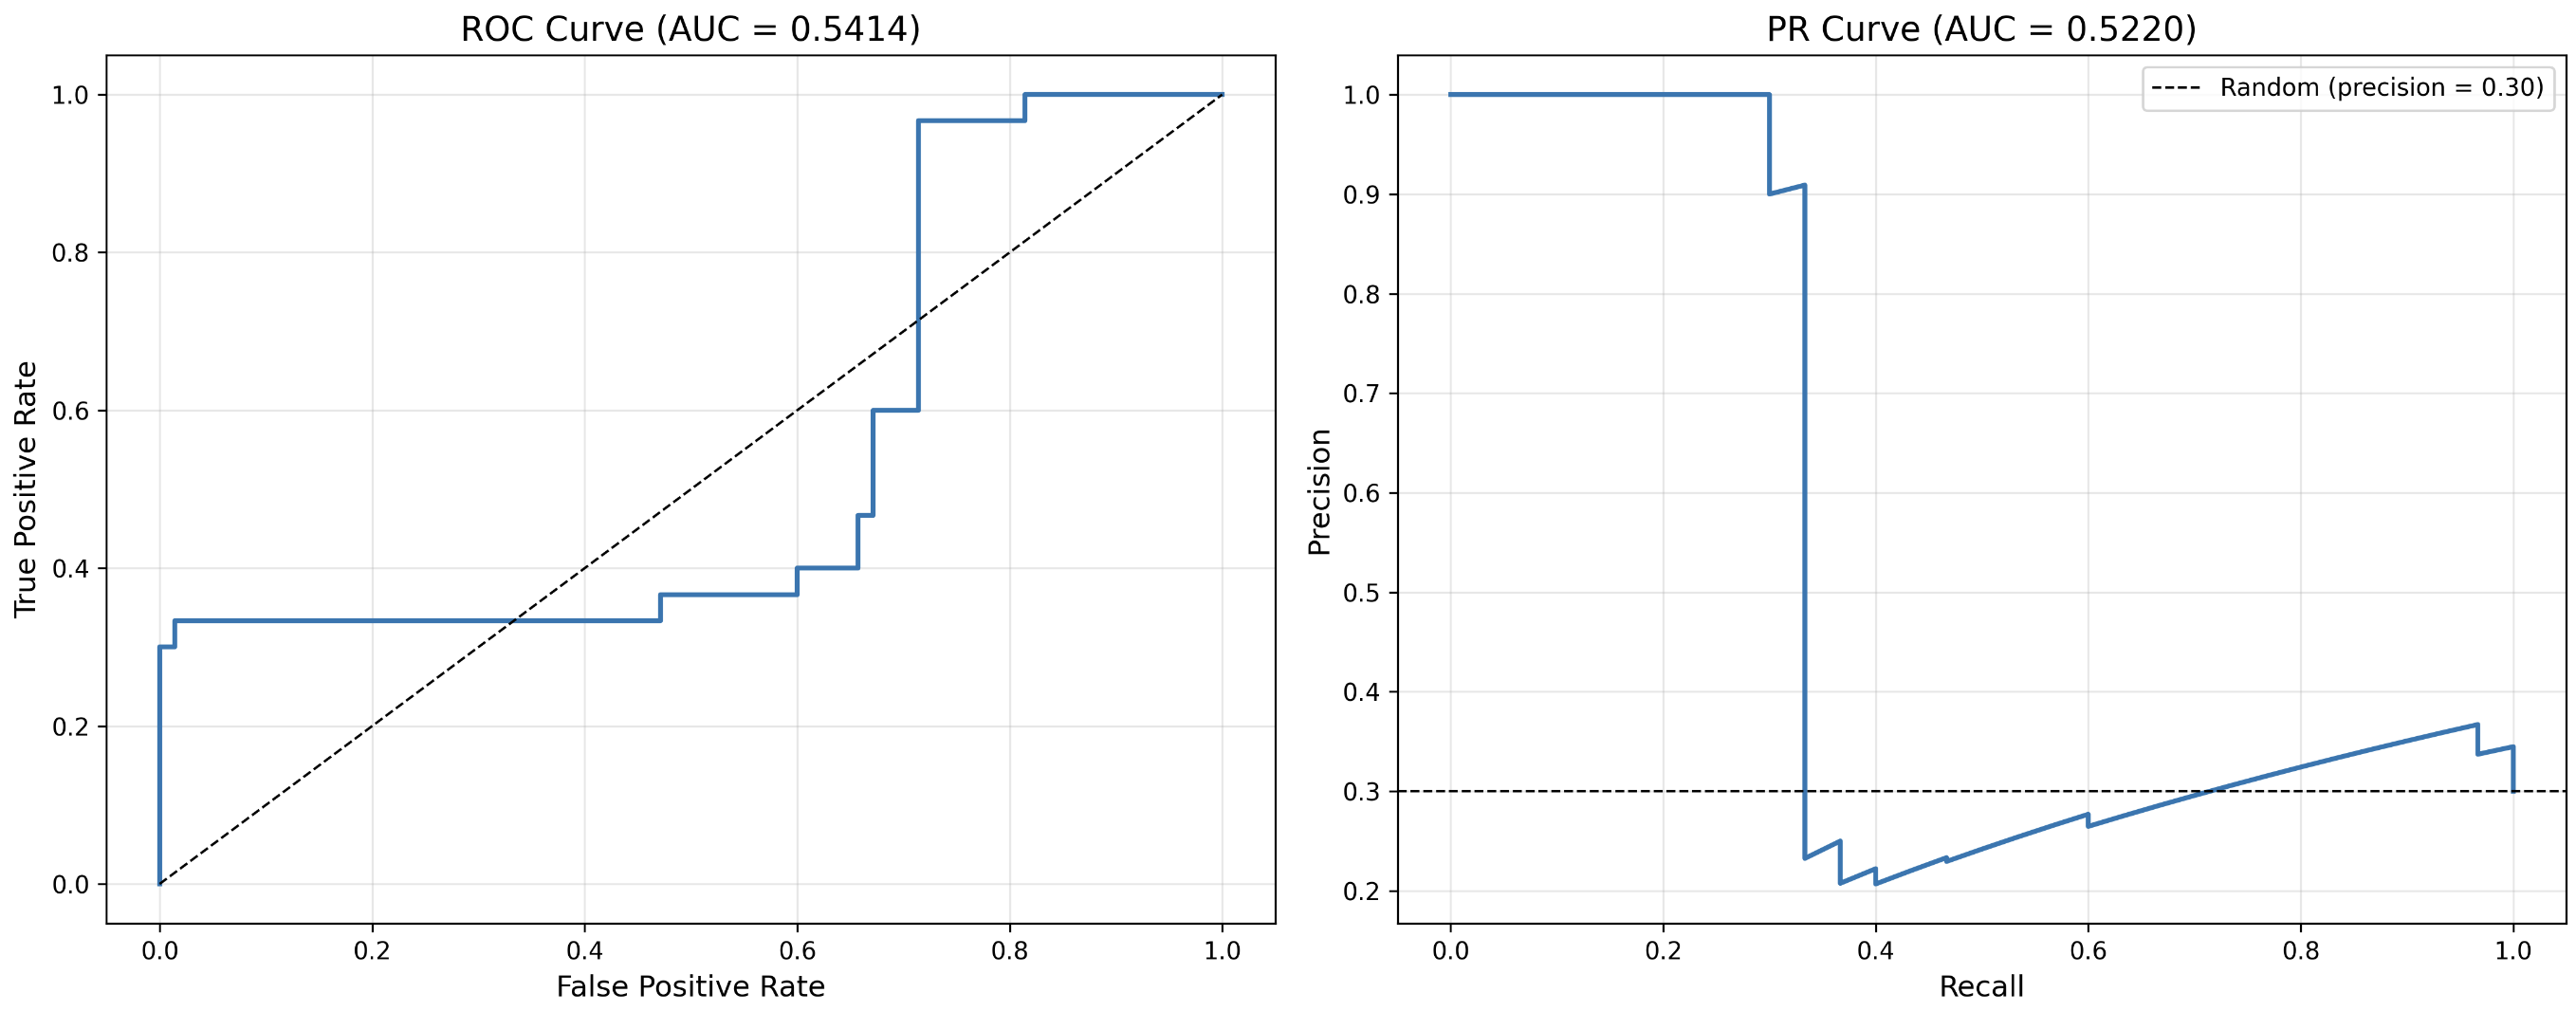
\includegraphics[width=\linewidth]{bright.png}
    \caption{Результат работы метода расслоенных пространств для задачи определения ярких пятен}
    \label{fig:bright}
  \end{minipage}
\end{figure}

\begin{figure}[ht]
  \centering
  \begin{minipage}[b]{0.9\linewidth} 
    \centering
    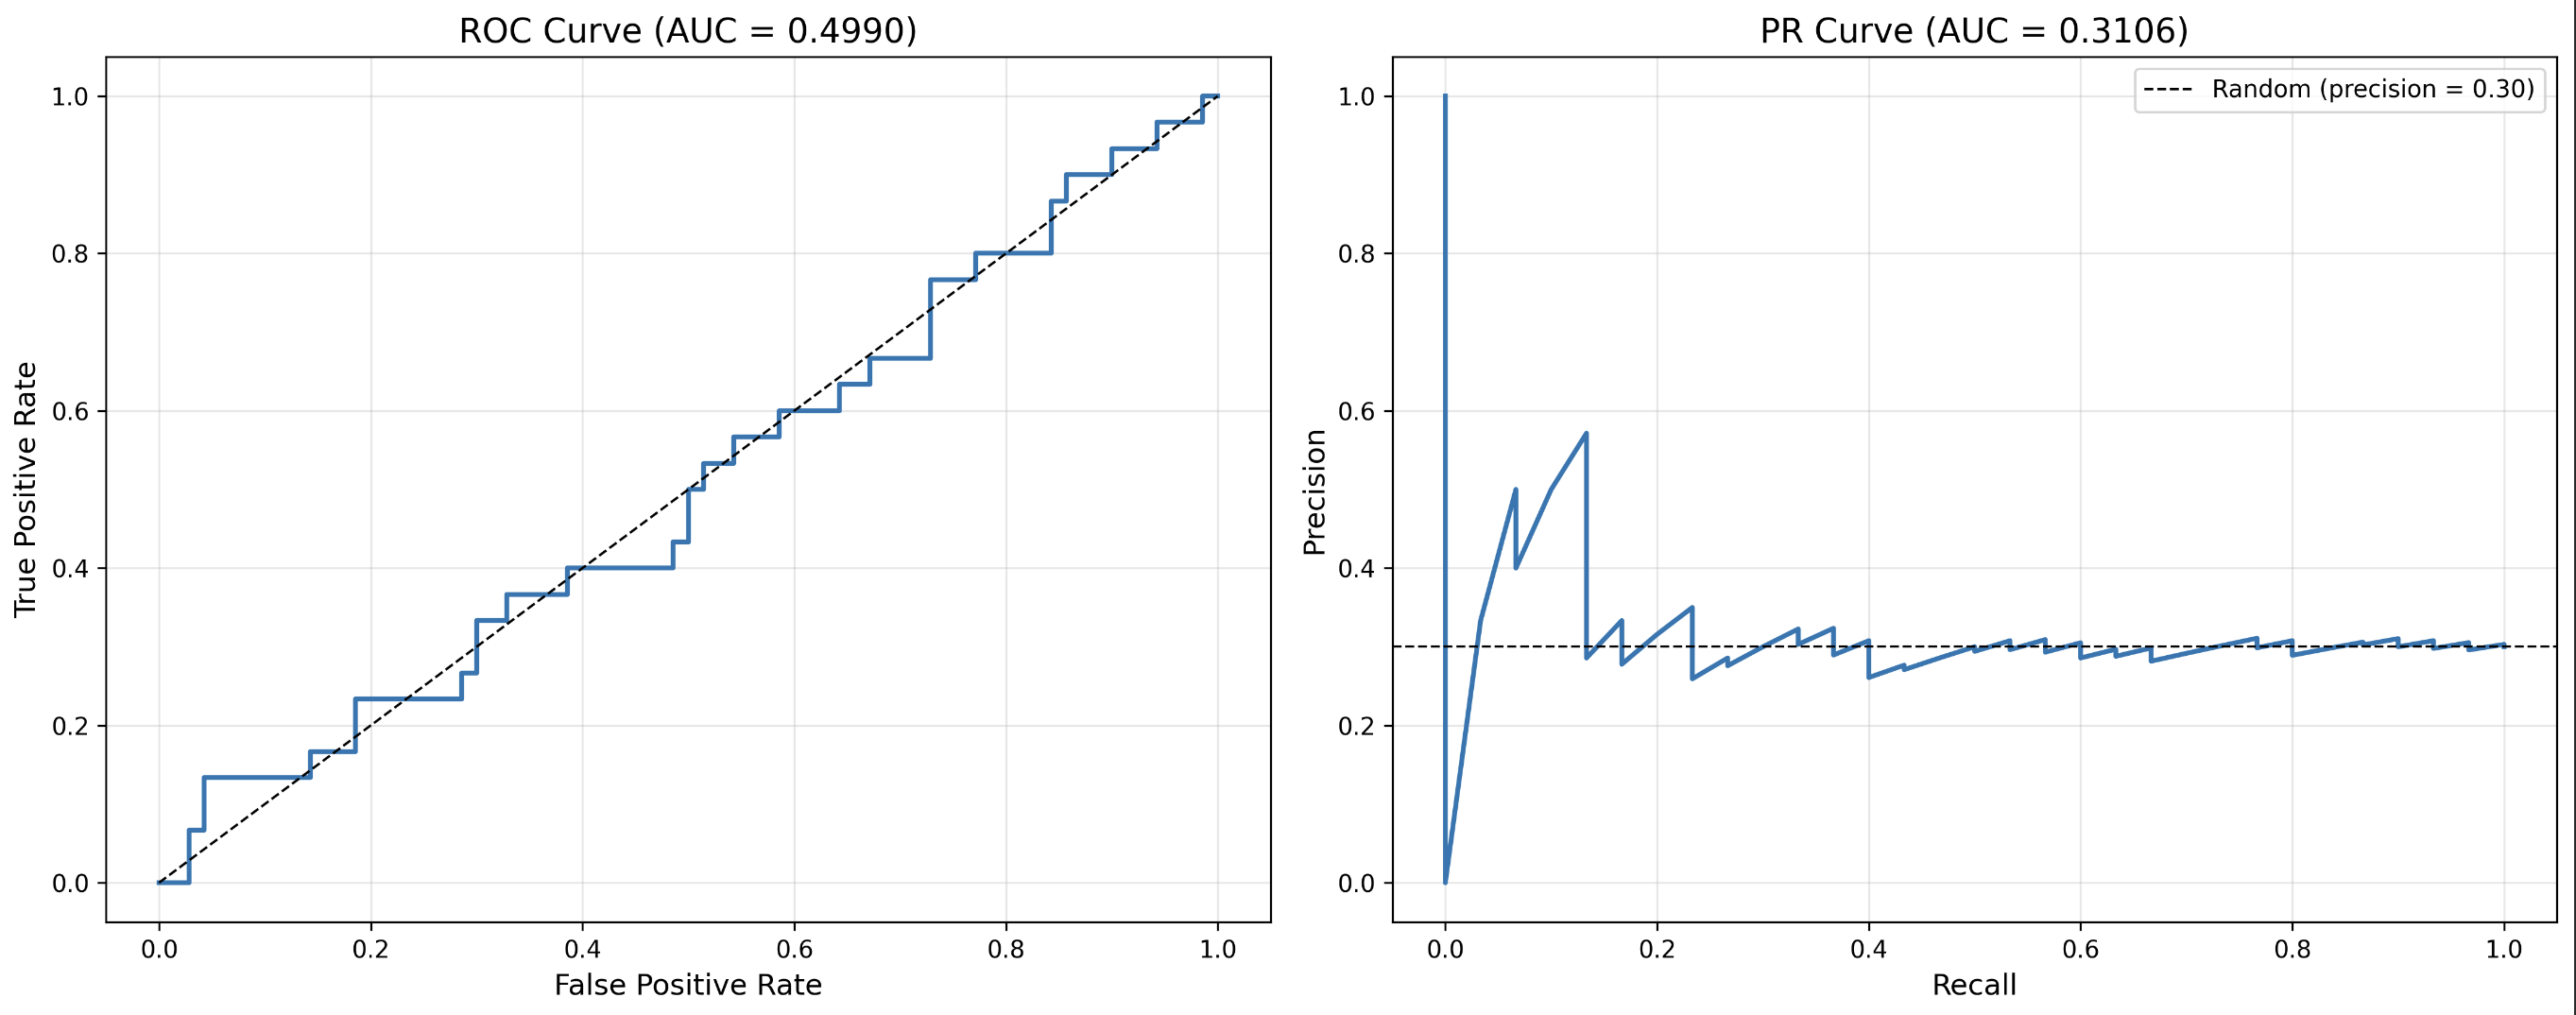
\includegraphics[width=\linewidth]{dark.png}
    \caption{Результат работы метода расслоенных пространств для задачи определения ярких пятен}
    \label{fig:dark}
  \end{minipage}
\end{figure}

\begin{figure}[ht]
  \centering
  \begin{minipage}[b]{0.9\linewidth} 
    \centering
    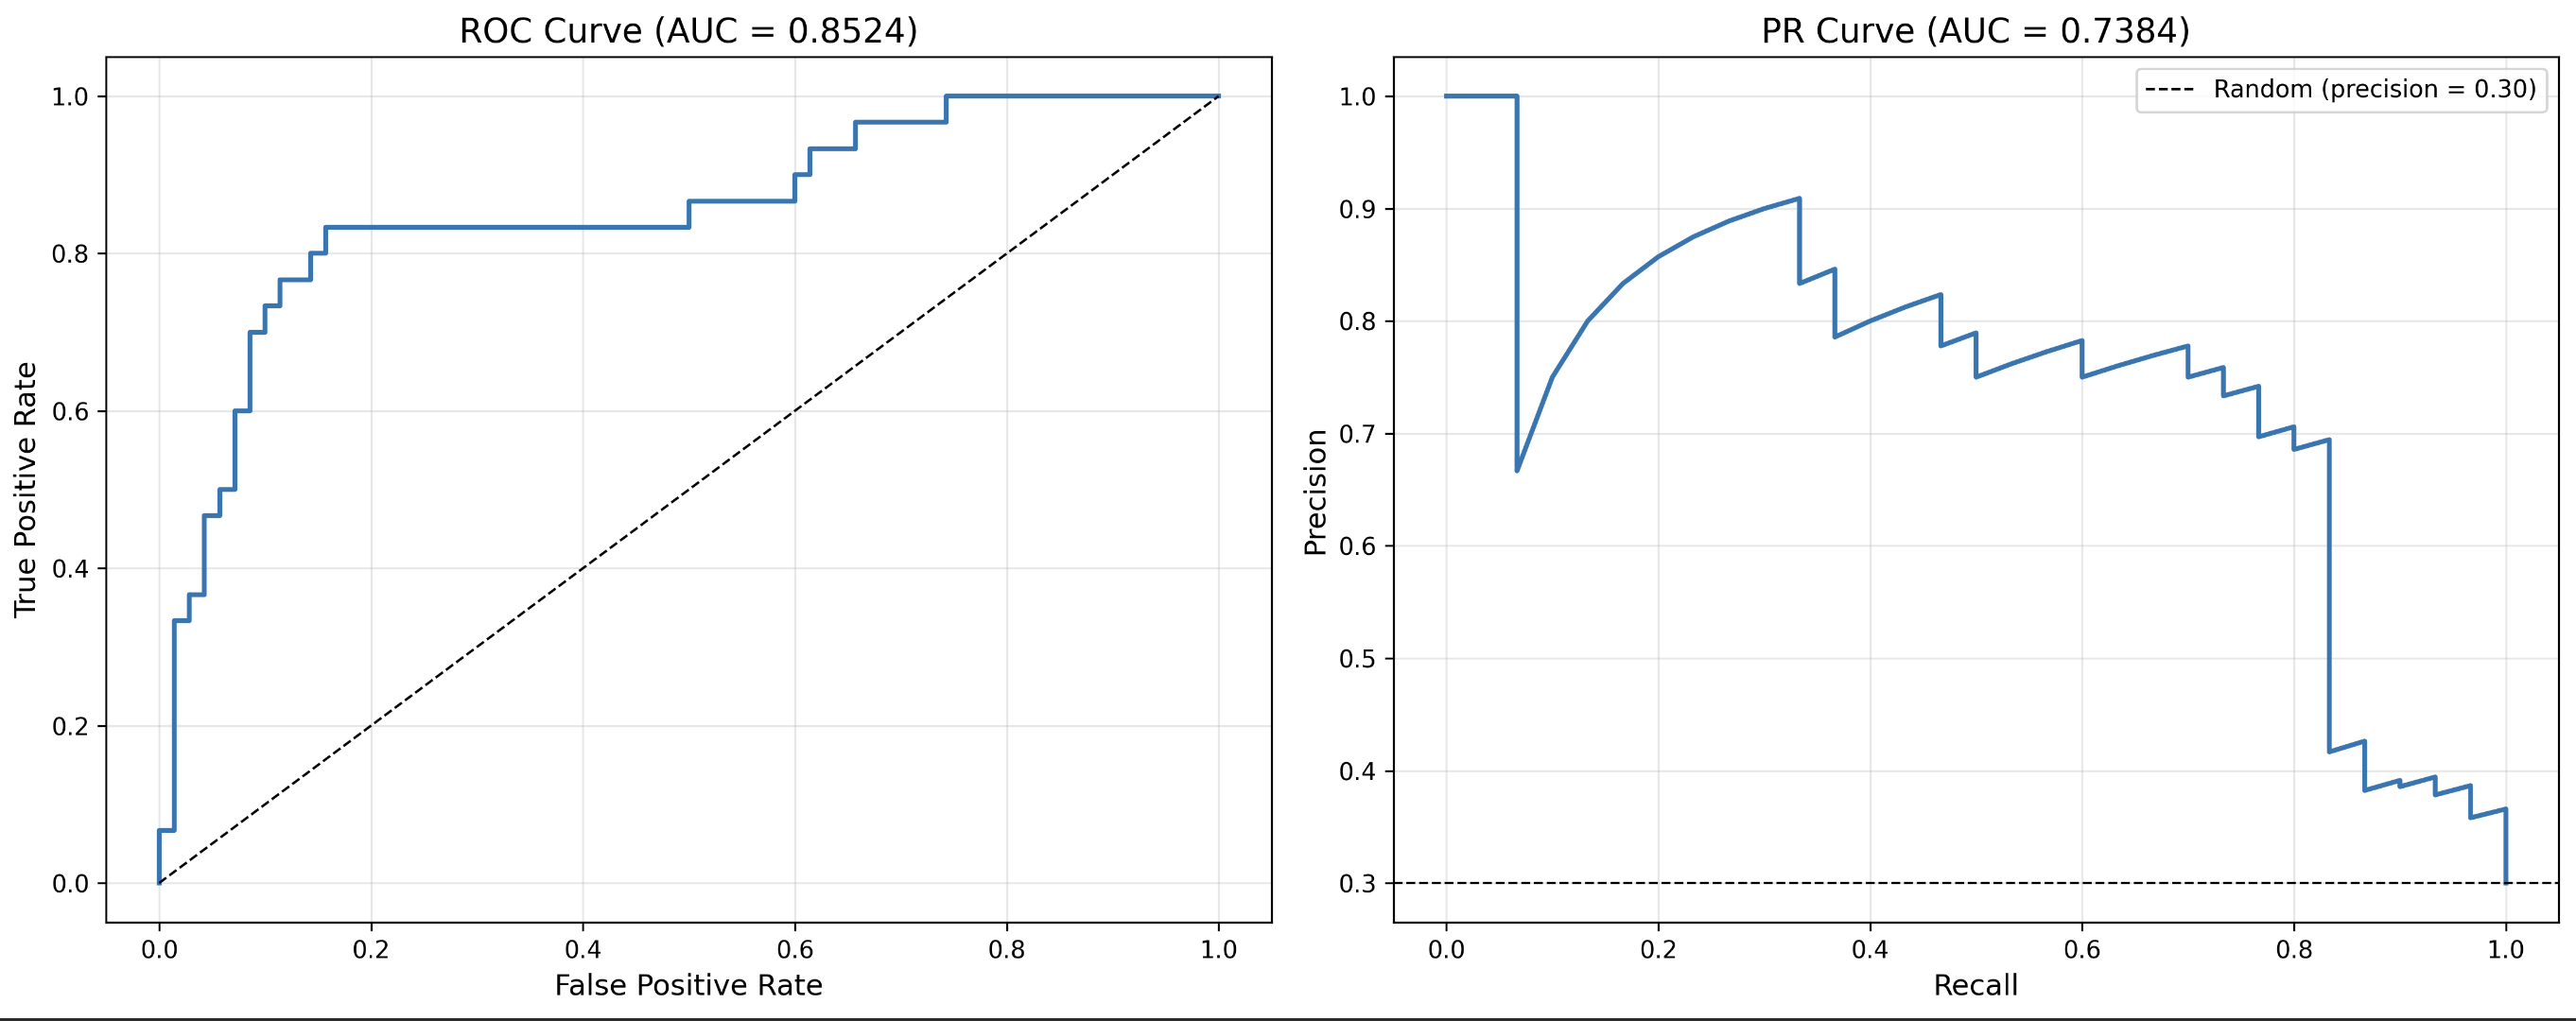
\includegraphics[width=\linewidth]{noise.png}
    \caption{Результат работы метода расслоенных пространств для задачи определения особенностей с шумом}
    \label{fig:noise}
  \end{minipage}
\end{figure}

\begin{figure}[ht]
  \centering
  \begin{minipage}[b]{0.9\linewidth} 
    \centering
    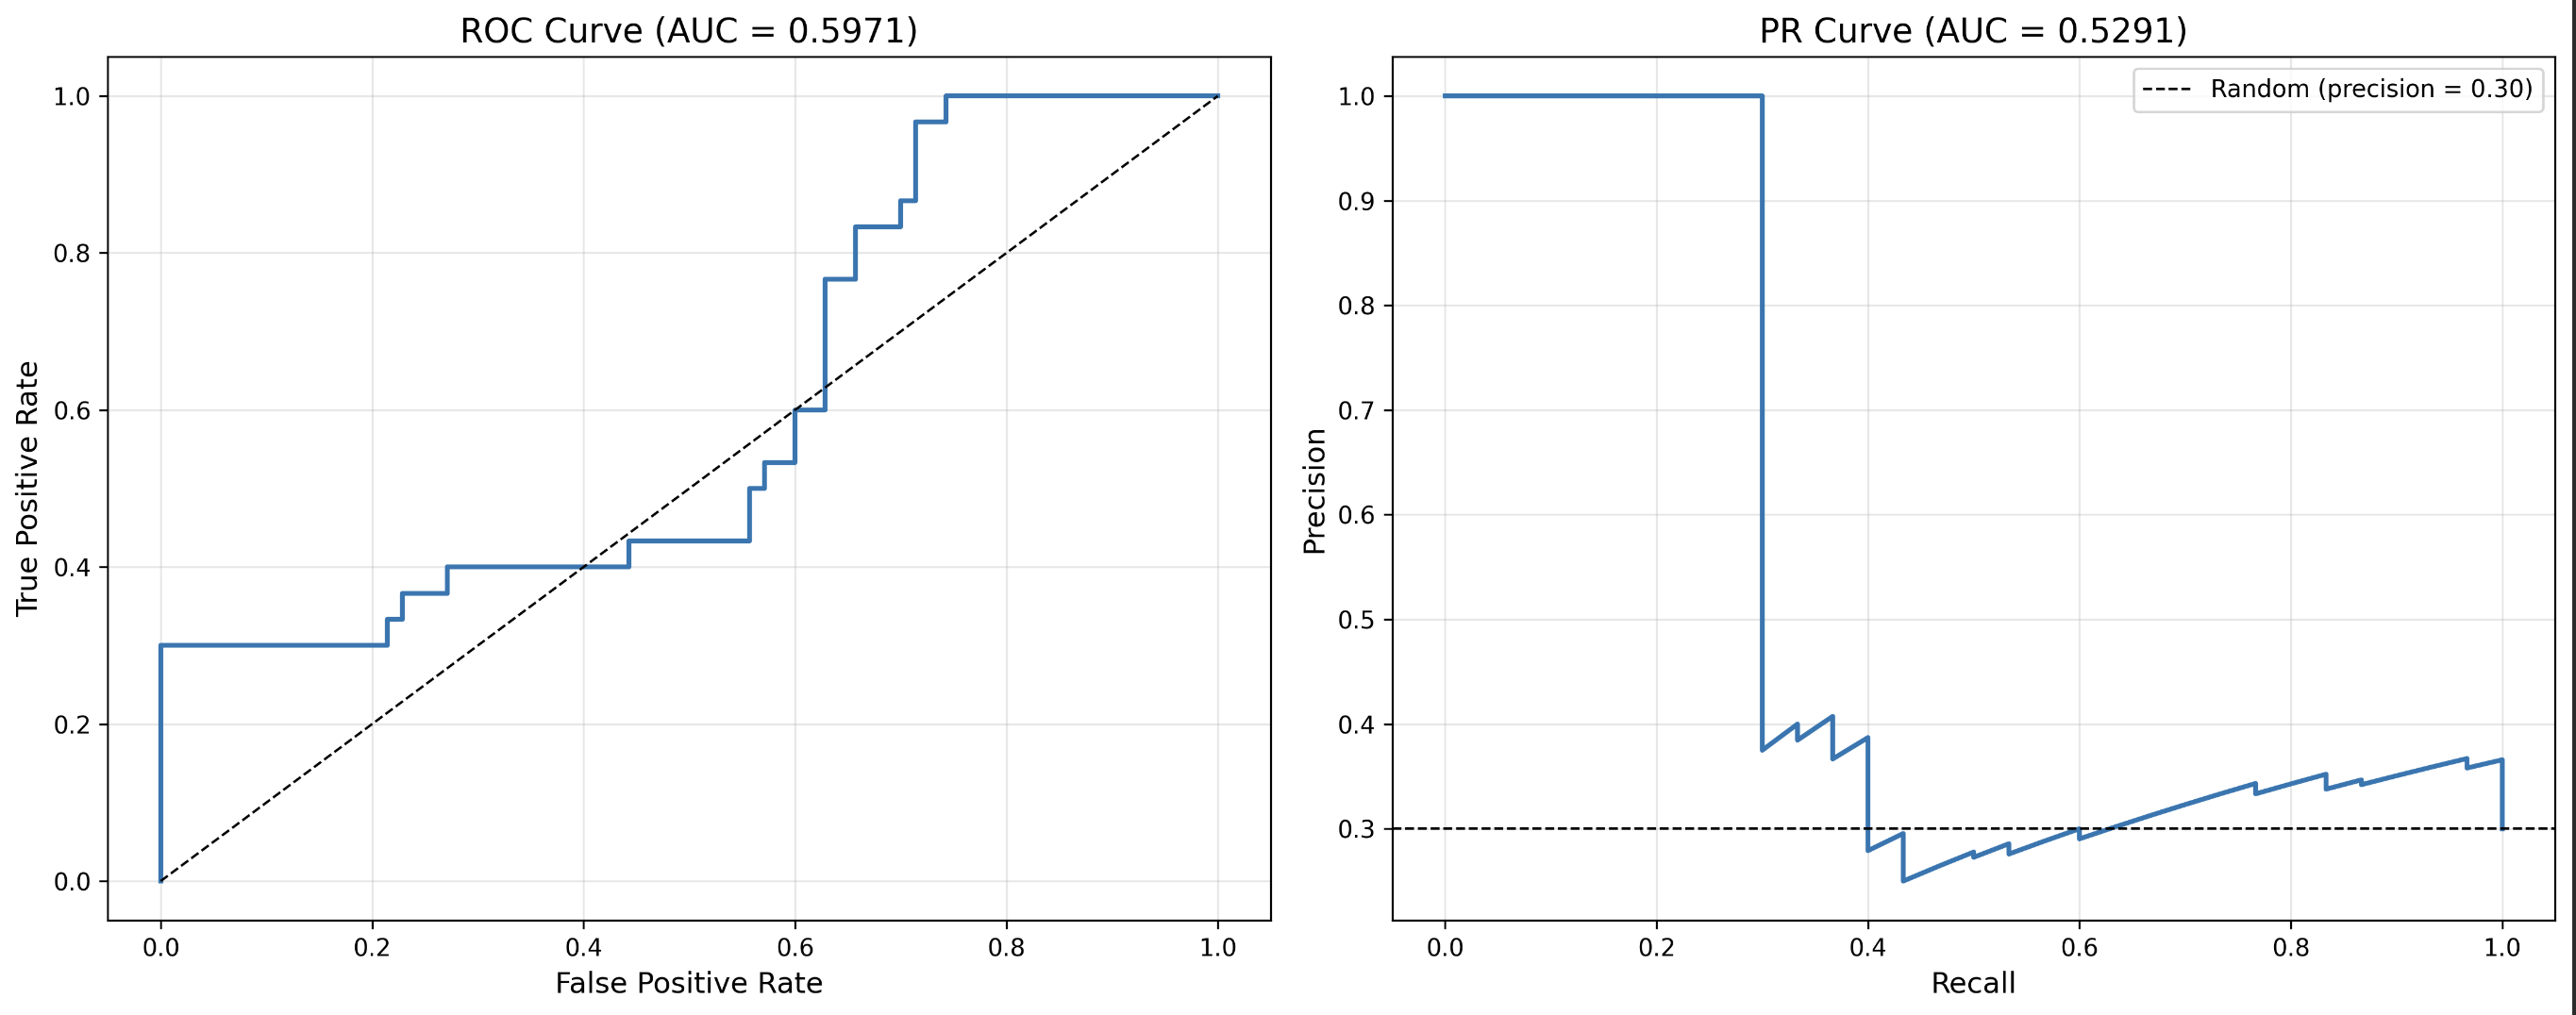
\includegraphics[width=\linewidth]{strips.png}
    \caption{Результат работы метода расслоенных пространств для задачи определения особенностей-полосок}
    \label{fig:strips}
  \end{minipage}
\end{figure}

Заметим, что для всех типов, кроме шума, значения метрик получились значимо ниже, чем при первоначальном замере, а значит имеет смысл провести эксперименты с разными гиперпаратрами для каждого типа особенности.

\subsection{Подбор гиперпараметров для различных типов особеннсотей}

Для улучшения метрик на каждом отдельном типе особенности подберем гиперпараметры. Будем руководствоваться знаниями о принципе работе метода и структуре каждого отдельно типа особенности: для ярких пятен стоит взять большое число соседей k из-за построения точек, а для темных пятен, наоборот, число соседей должно быть небольшим. Аналогично для особенностей с шумом количество соседей должно быть небольшим, причем размерность n\_pca, до которой мы уменьшаем пространство, тоже должна быть небольшой. Для особенностей-полосок из-за вида этой особенности мы должны брать большое значение k. 

Итого, после обновления гиперпараметров мы получаем новые значения метрик. Графики со значениями метрик для ярких пятен можно увидеть на рисунке ~\ref{fig:bright_new}, для темных пятен на рисунке ~\ref{fig:dark_new}, для особенностей с шумом на рисунке ~\ref{fig:noise_new}, для особенностей-полосок на рисунке ~\ref{fig:strips_new}.

\begin{figure}[ht]
  \centering
  \begin{minipage}[b]{0.9\linewidth} 
    \centering
    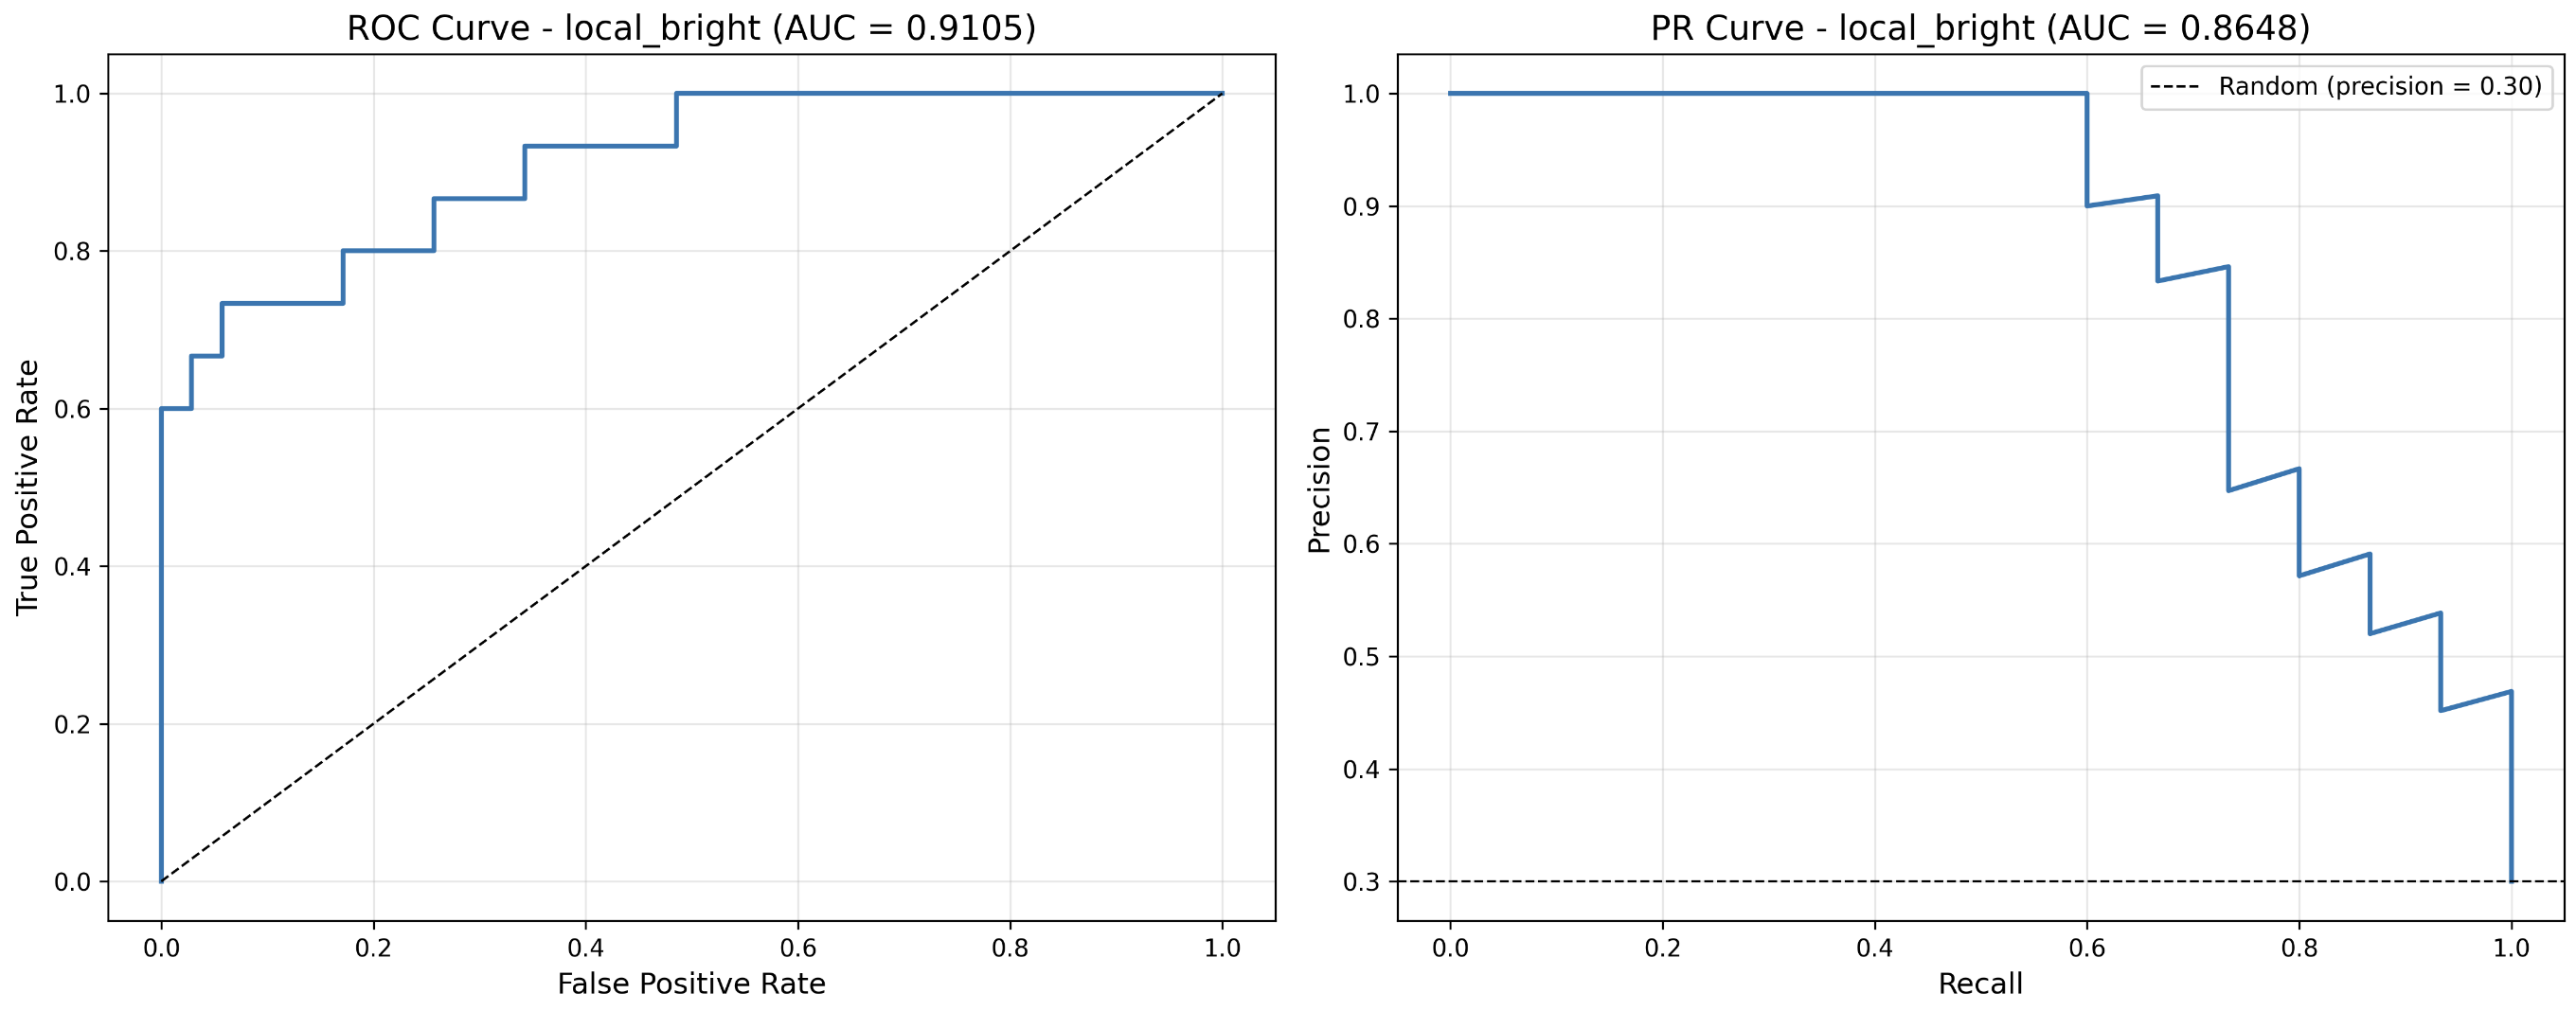
\includegraphics[width=\linewidth]{bright_new.png}
    \caption{Результат работы метода расслоенных пространств для задачи определения ярких пятен (после подбора гиперпараметров)}
    \label{fig:bright_new}
  \end{minipage}
\end{figure}

\begin{figure}[ht]
  \centering
  \begin{minipage}[b]{0.9\linewidth} 
    \centering
    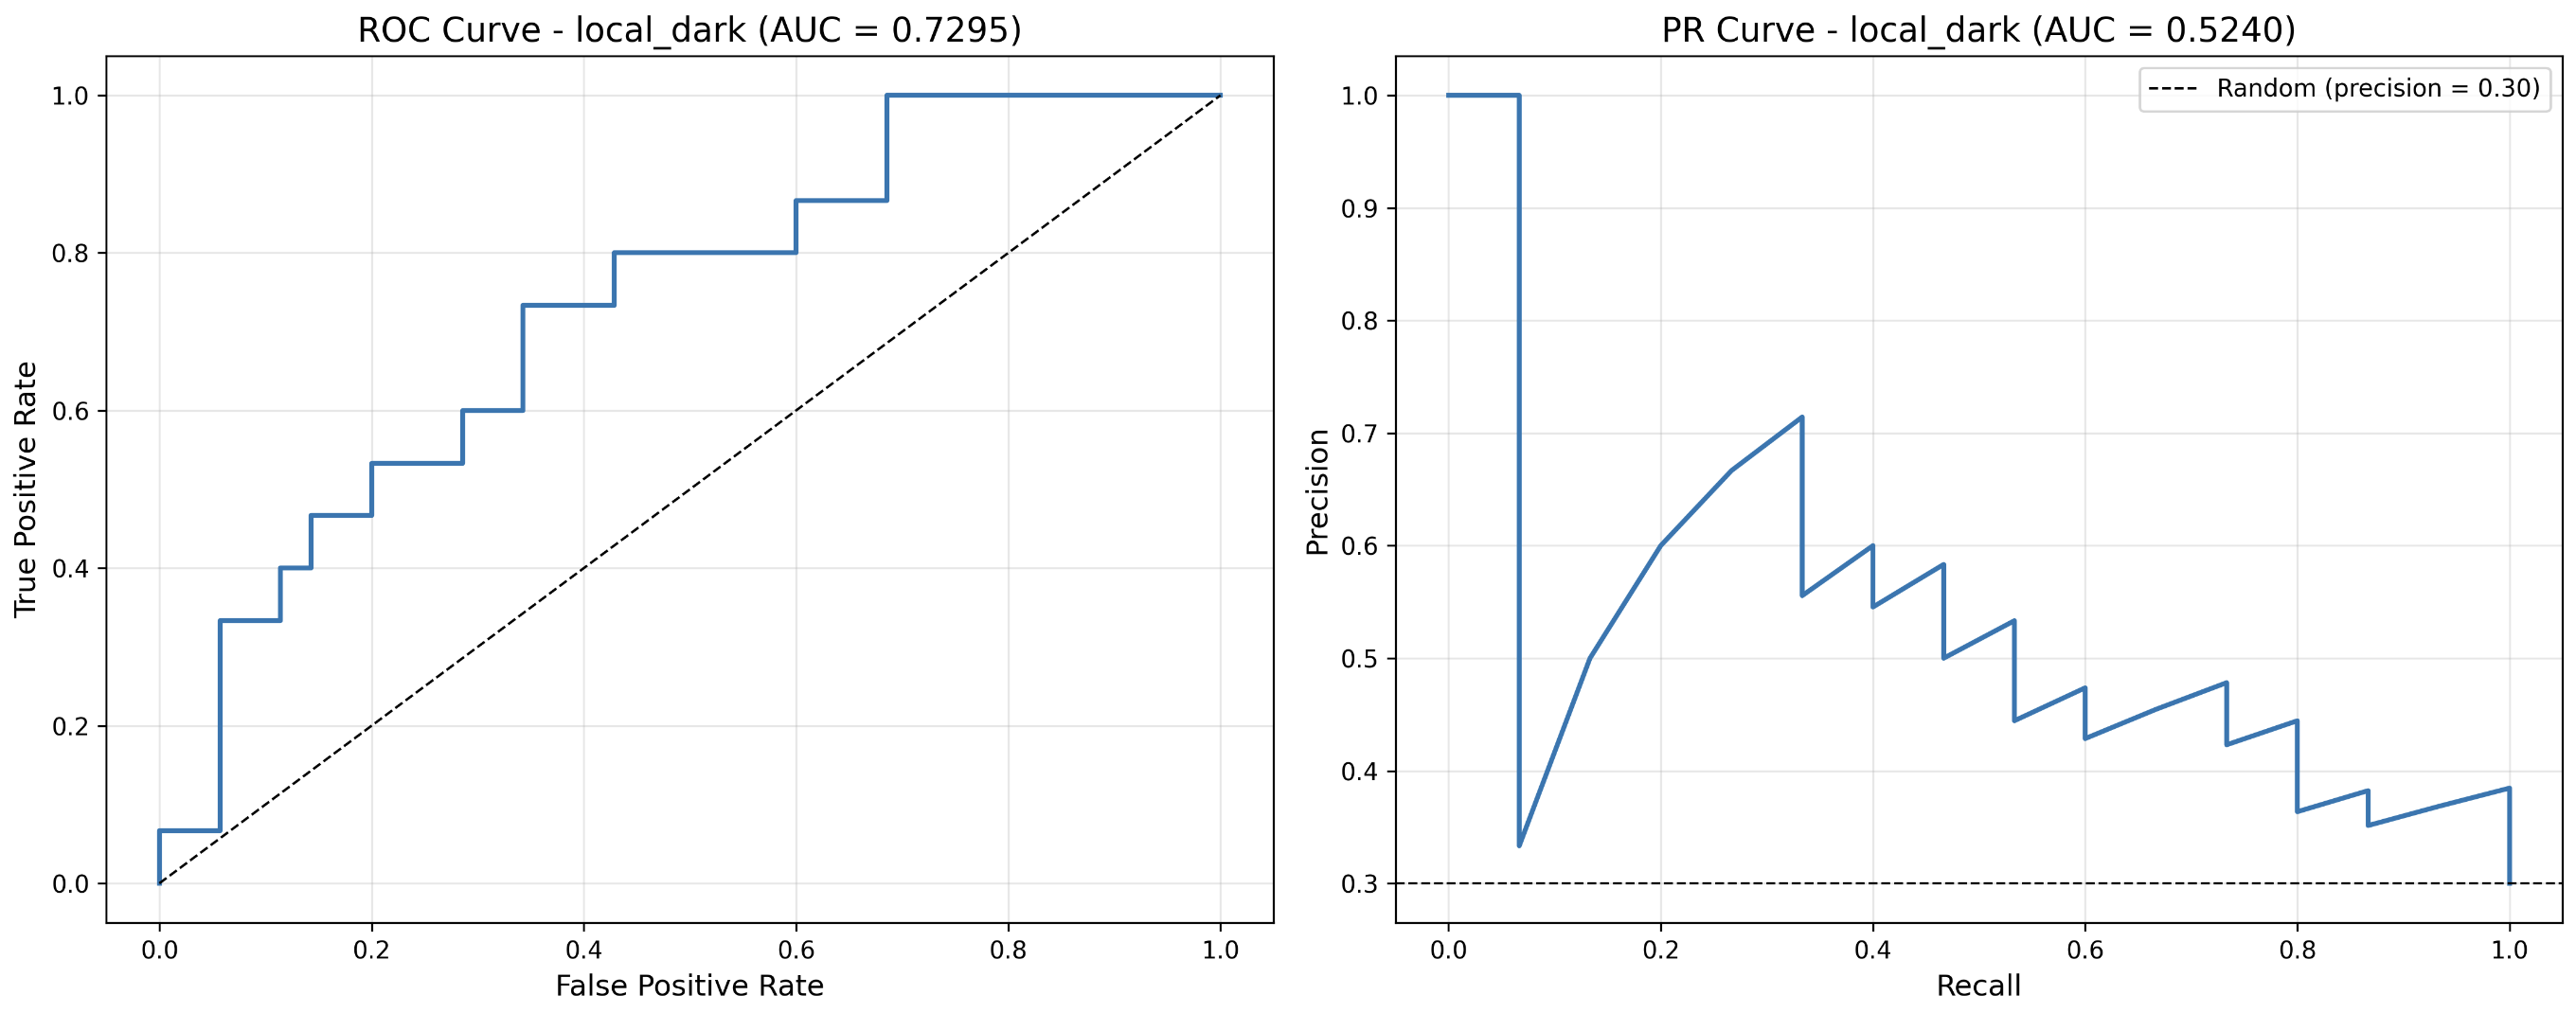
\includegraphics[width=\linewidth]{dark_new.png}
    \caption{Результат работы метода расслоенных пространств для задачи определения ярких пятен (после подбора гиперпараметров)}
    \label{fig:dark_new}
  \end{minipage}
\end{figure}

\begin{figure}[ht]
  \centering
  \begin{minipage}[b]{0.9\linewidth} 
    \centering
    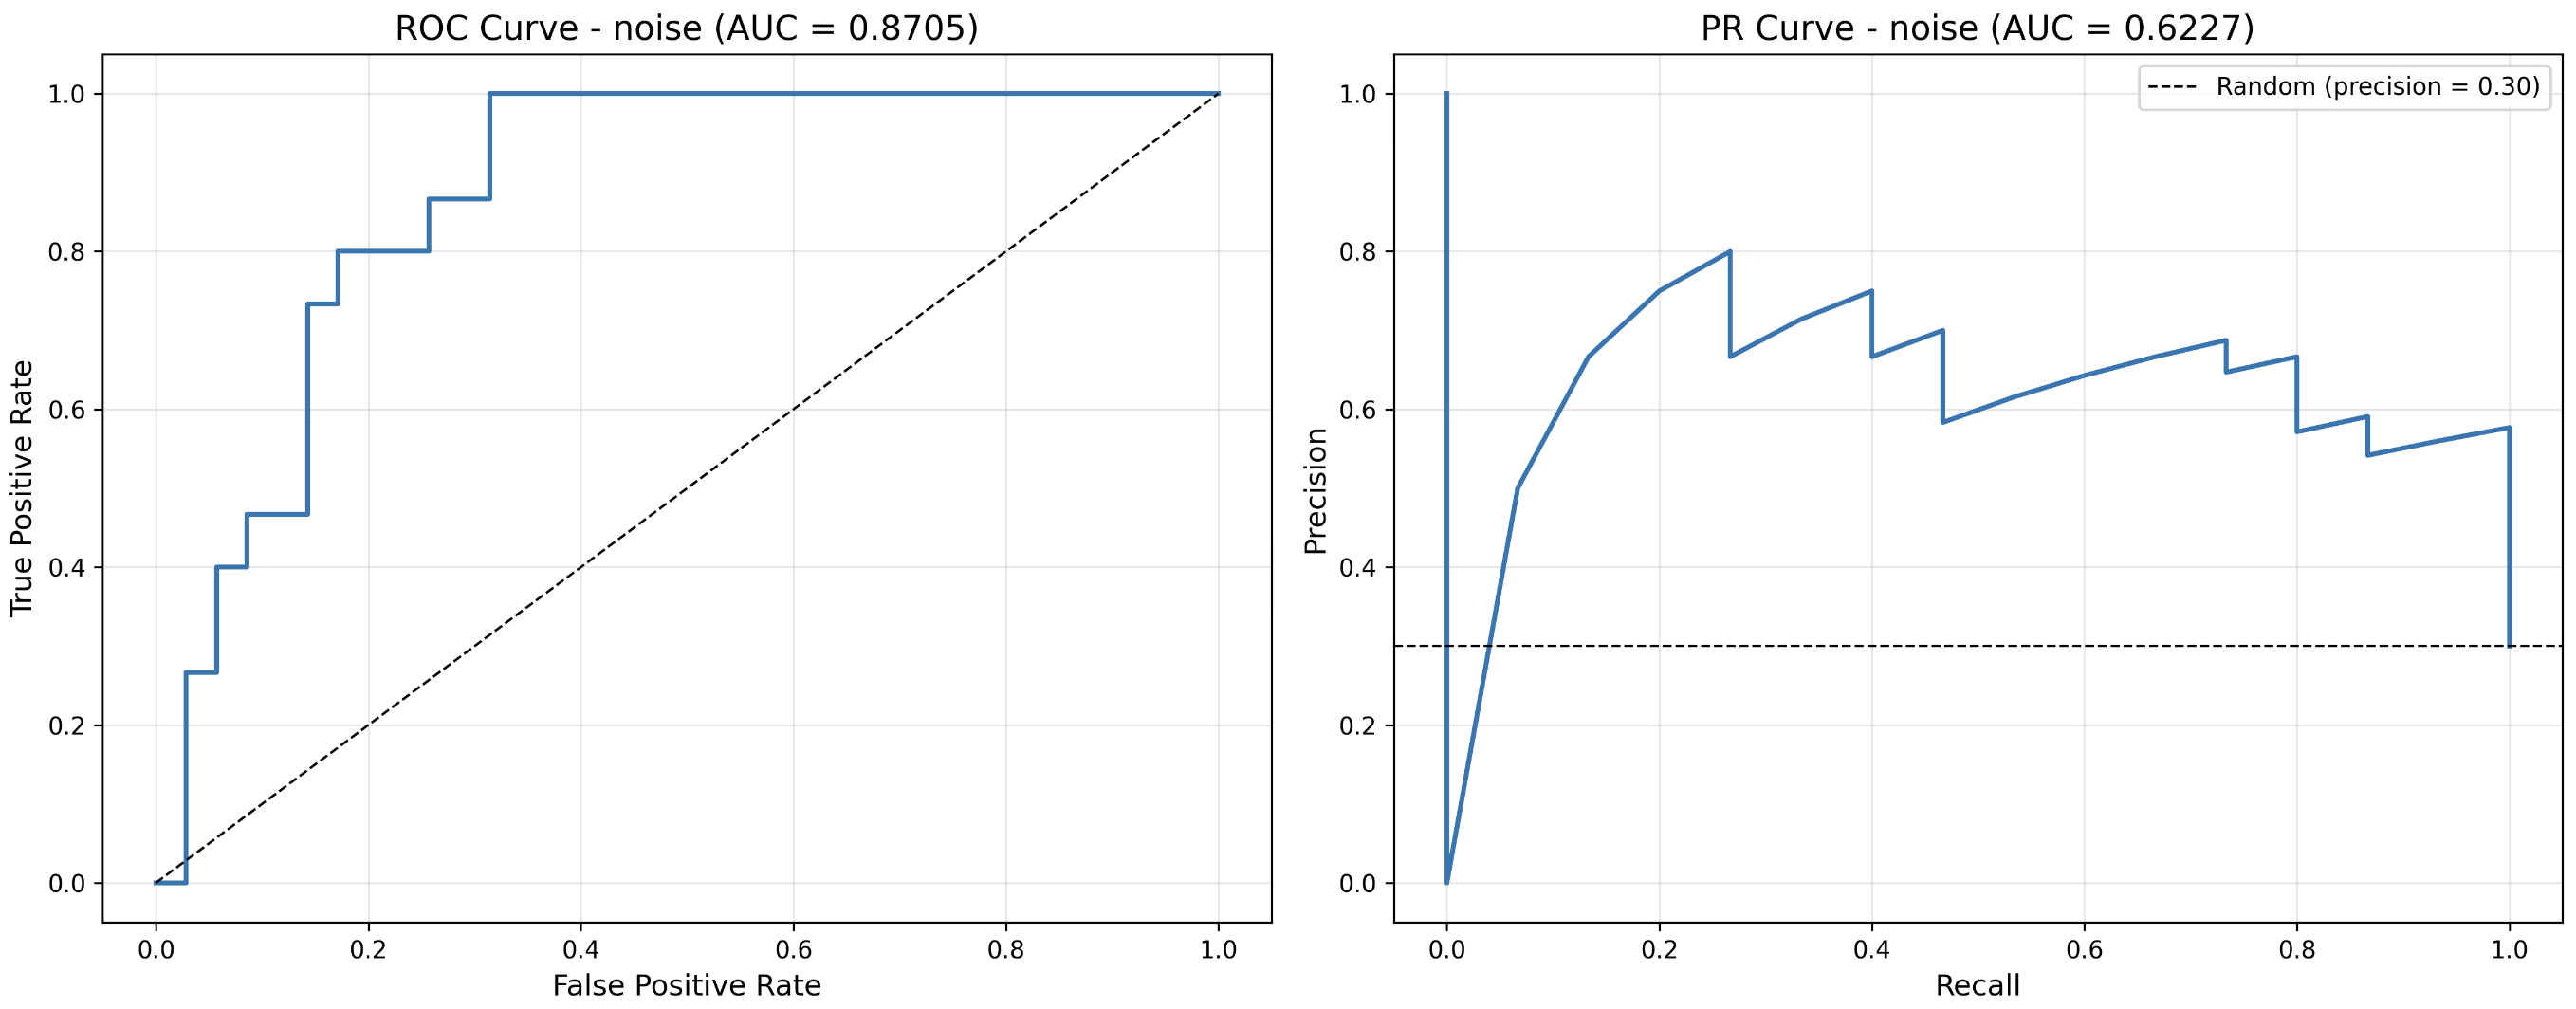
\includegraphics[width=\linewidth]{noise_new.png}
    \caption{Результат работы метода расслоенных пространств для задачи определения особенностей с шумом (после подбора гиперпараметров)}
    \label{fig:noise_new}
  \end{minipage}
\end{figure}

\begin{figure}[ht]
  \centering
  \begin{minipage}[b]{0.9\linewidth} 
    \centering
    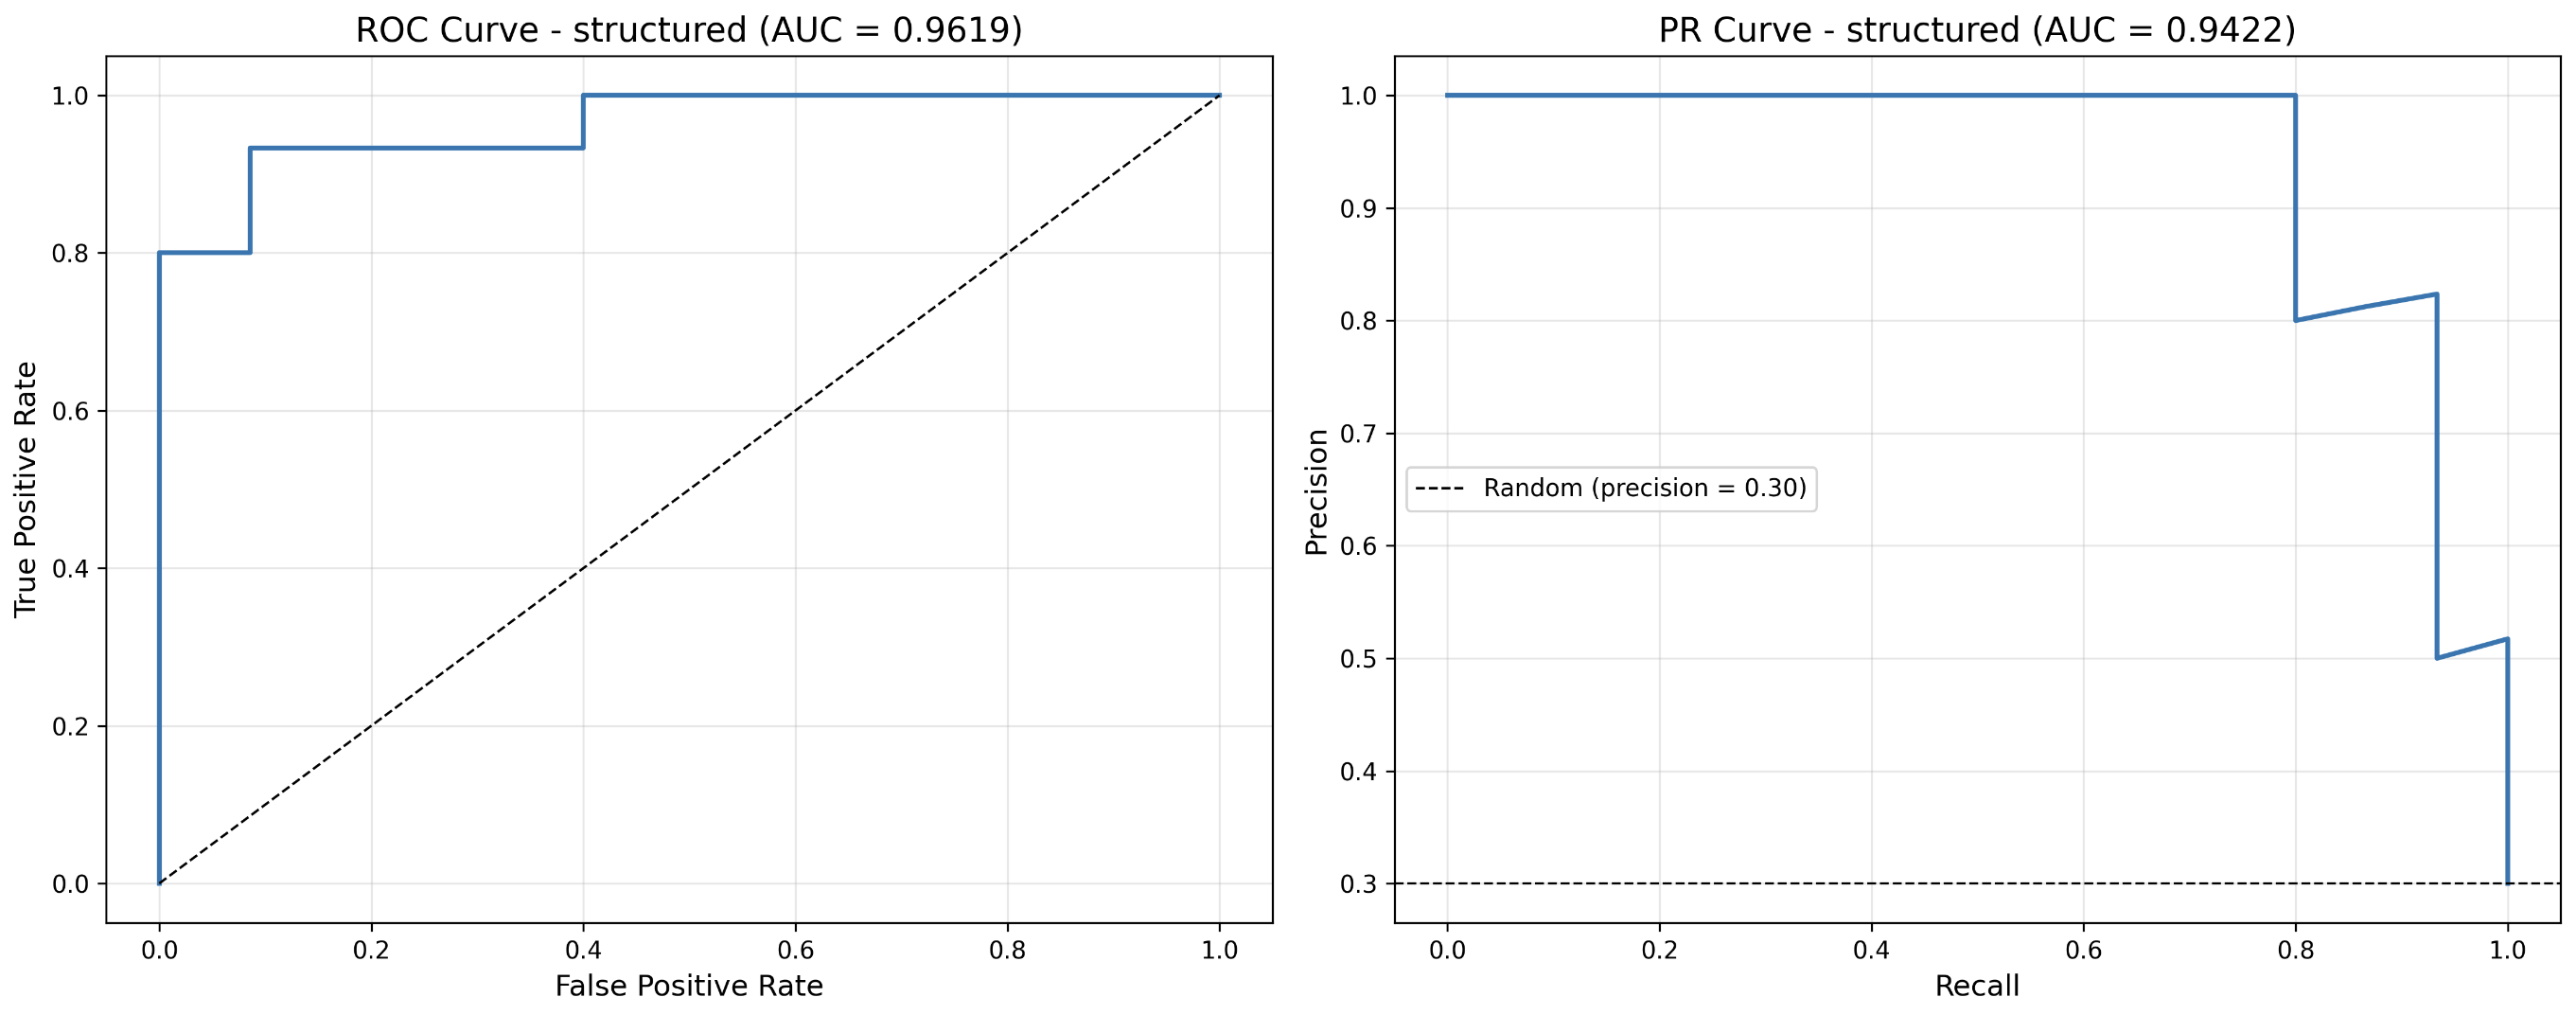
\includegraphics[width=\linewidth]{strips_new.png}
    \caption{Результат работы метода расслоенных пространств для задачи определения особенностей-полосок (после подбора гиперпараметров)}
    \label{fig:strips_new}
  \end{minipage}
\end{figure}

Можно заметить, что после подбора гиперпараметров значение метрик сильно увеличилось для всех типов особенностей.

\section{Применение модели для построения маски опухоли}

\subsection{Выбор датасета}

В предыдущих разделах мы убедились, что предложенный метод хорошо работает на синтетических примерах, причем до этого мы проверяли корректность бинарного вердикта с наличием особенности на снимке. Теперь необходимо замерить качество подхода на примерах с опухолями и измерить качество выделения особенностей на снимках. Для этой задачи будем использовать датасет из соревнования Brain Tumor Segmentation (BraTS)\footnote{Соревнование и датасет доступны по ссылке: \url{http://braintumorsegmentation.org}, дата обр. 25.04.2025}, который содержит снимки с выделенными аномалиями на МРТ-снимках. Применим наш метод на этих данных, выделим найденные аномалии и замерим метрику IoU (Intersection over Union)[28], которая попиксельно сравнивает выделенные области. Пример изображений, полученных из данных этого датасета, можно увидеть на рисунке~\ref{fig:MGMT}.

\begin{figure}[ht]
  \centering
  \begin{minipage}[b]{0.9\linewidth} 
    \centering
    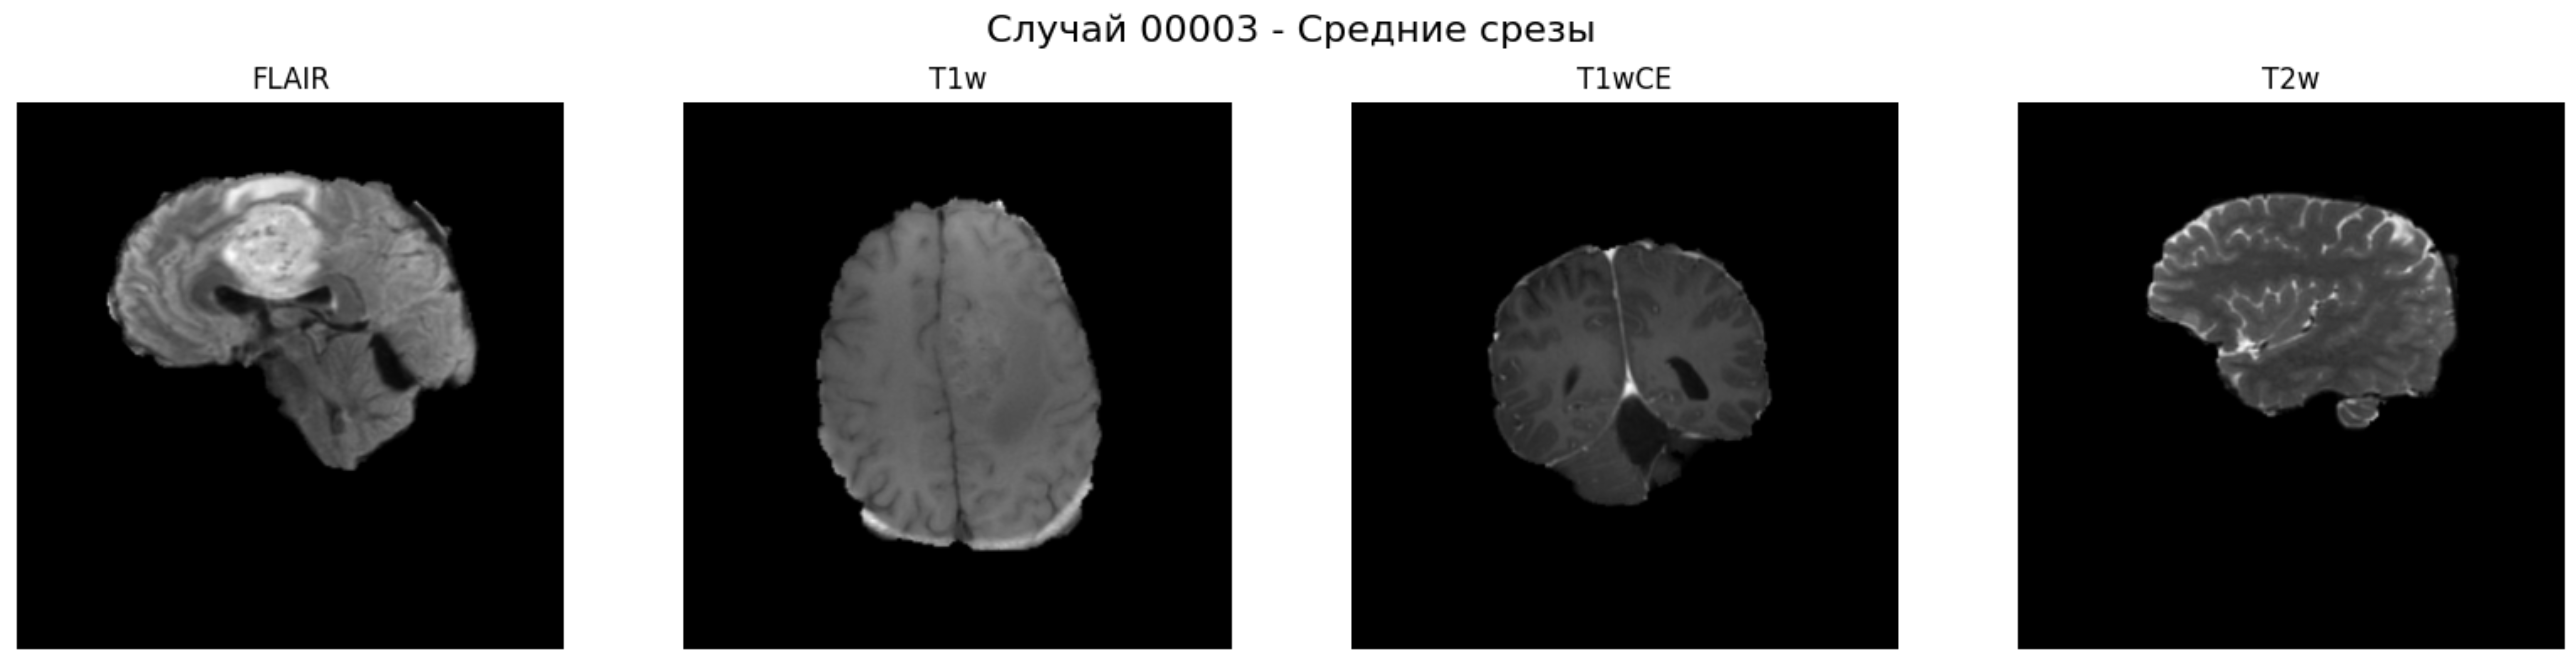
\includegraphics[width=\linewidth]{MGMT.png}
    \caption{Пример снимков из датасета BraTS}
    \label{fig:MGMT}
  \end{minipage}
\end{figure}

Данные изображения можно представить в виде изображения мозга и отмеченной особенности (маски опухоли). Пример можно увидеть на рисунке~\ref{fig:tumor_and_mask}. Объединив маску и МРТ-снимок, мы получим изображение, которое можно увидеть на рисунке~\ref{fig:tumor_and_mask_2}. Наша задача будет заключаться в том, чтобы по снимку выделить маску и сравнить предсказанную и истинную маски. В итоге мы получим значение метрики IoU. 

\begin{figure}[ht]
  \centering
  \begin{minipage}[b]{0.9\linewidth} 
    \centering
    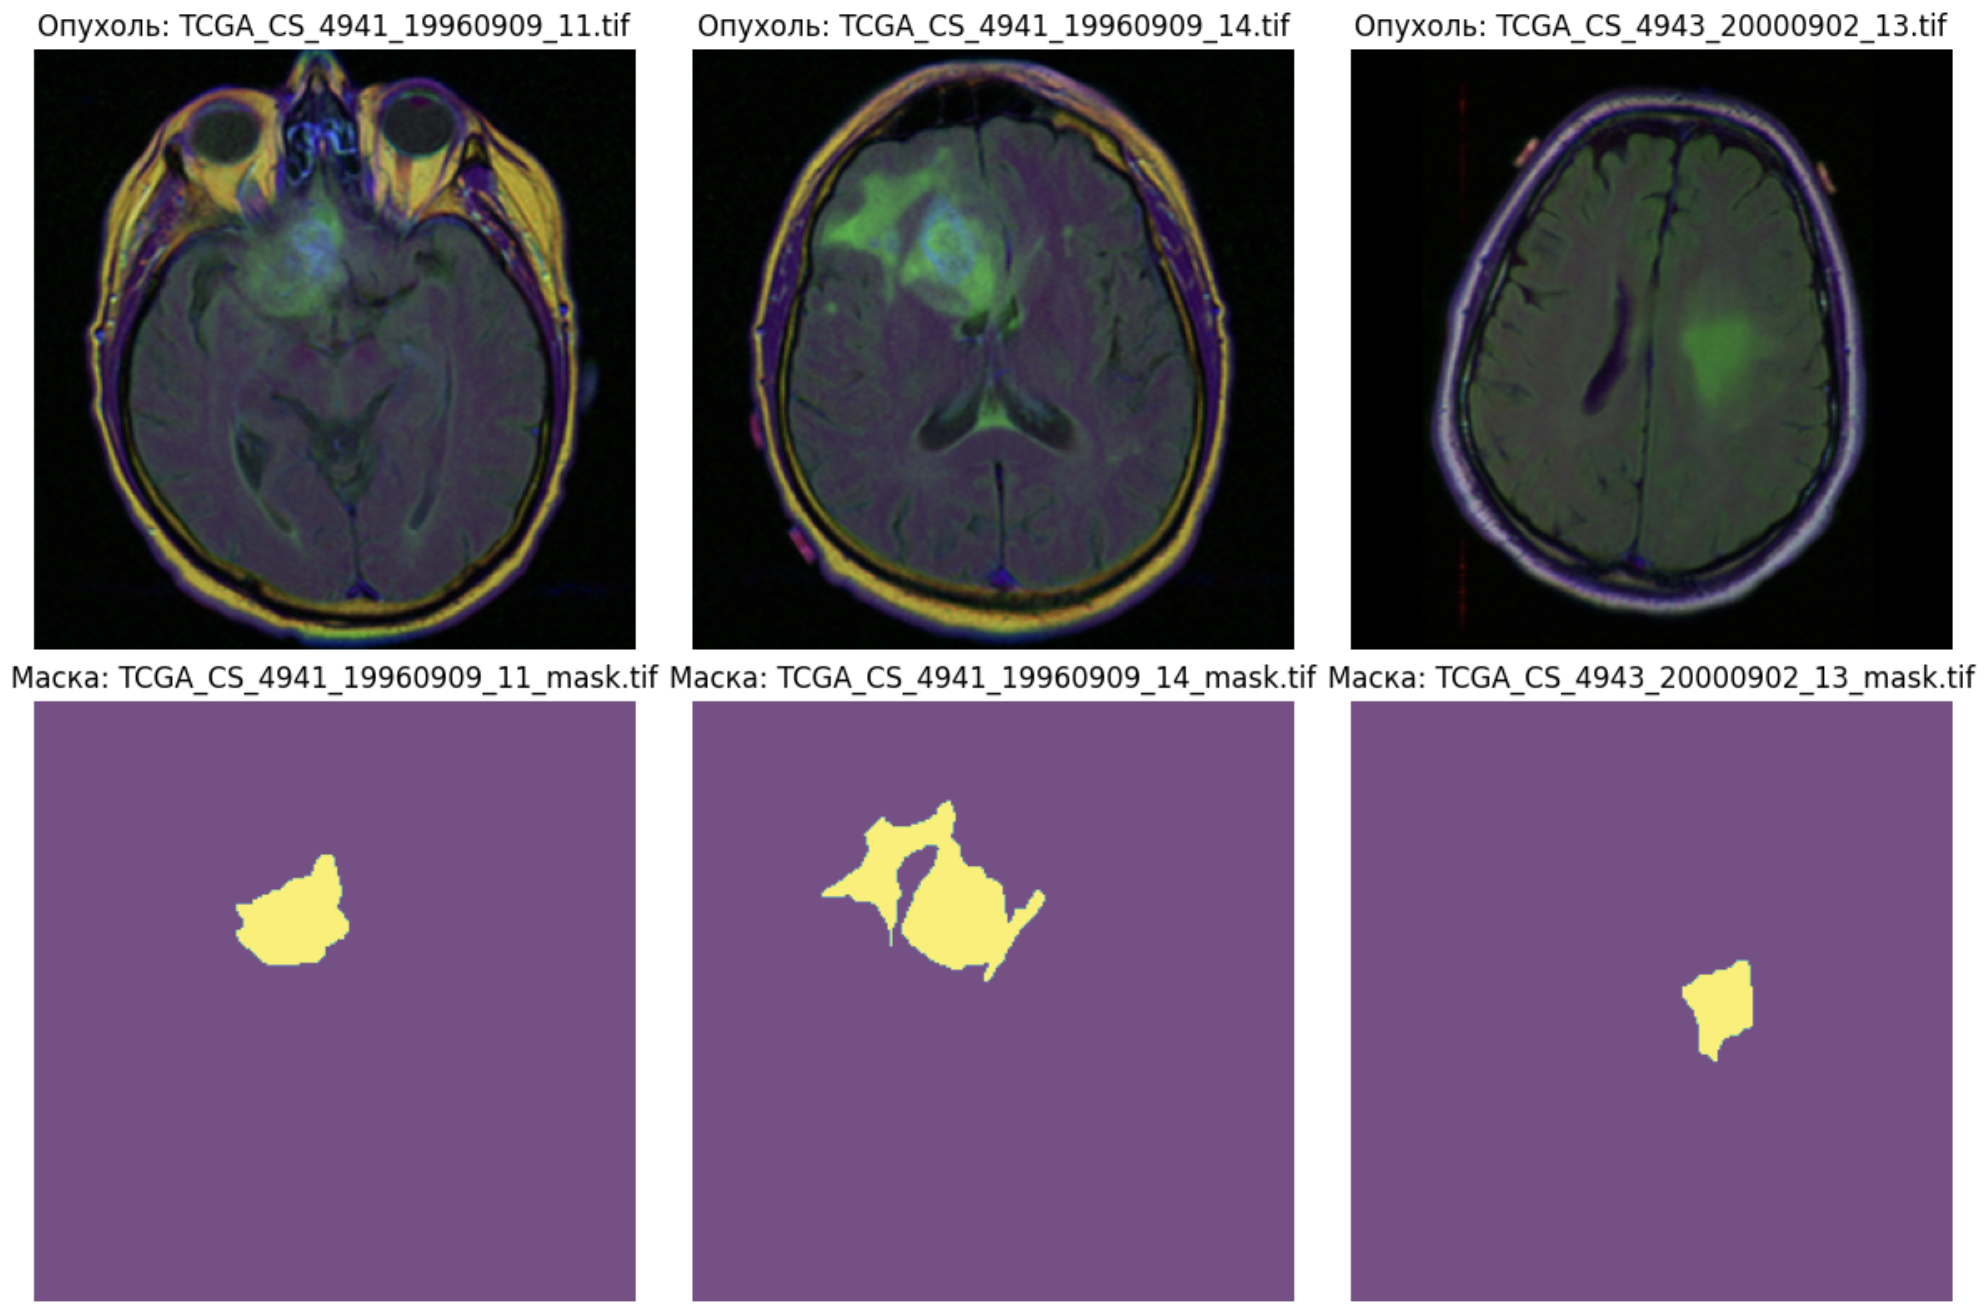
\includegraphics[width=\linewidth]{tumor_and_mask.png}
    \caption{Пример снимка и маски из датасета BraTS}
    \label{fig:tumor_and_mask}
  \end{minipage}
\end{figure}

\begin{figure}[ht]
  \centering
  \begin{minipage}[b]{0.9\linewidth} 
    \centering
    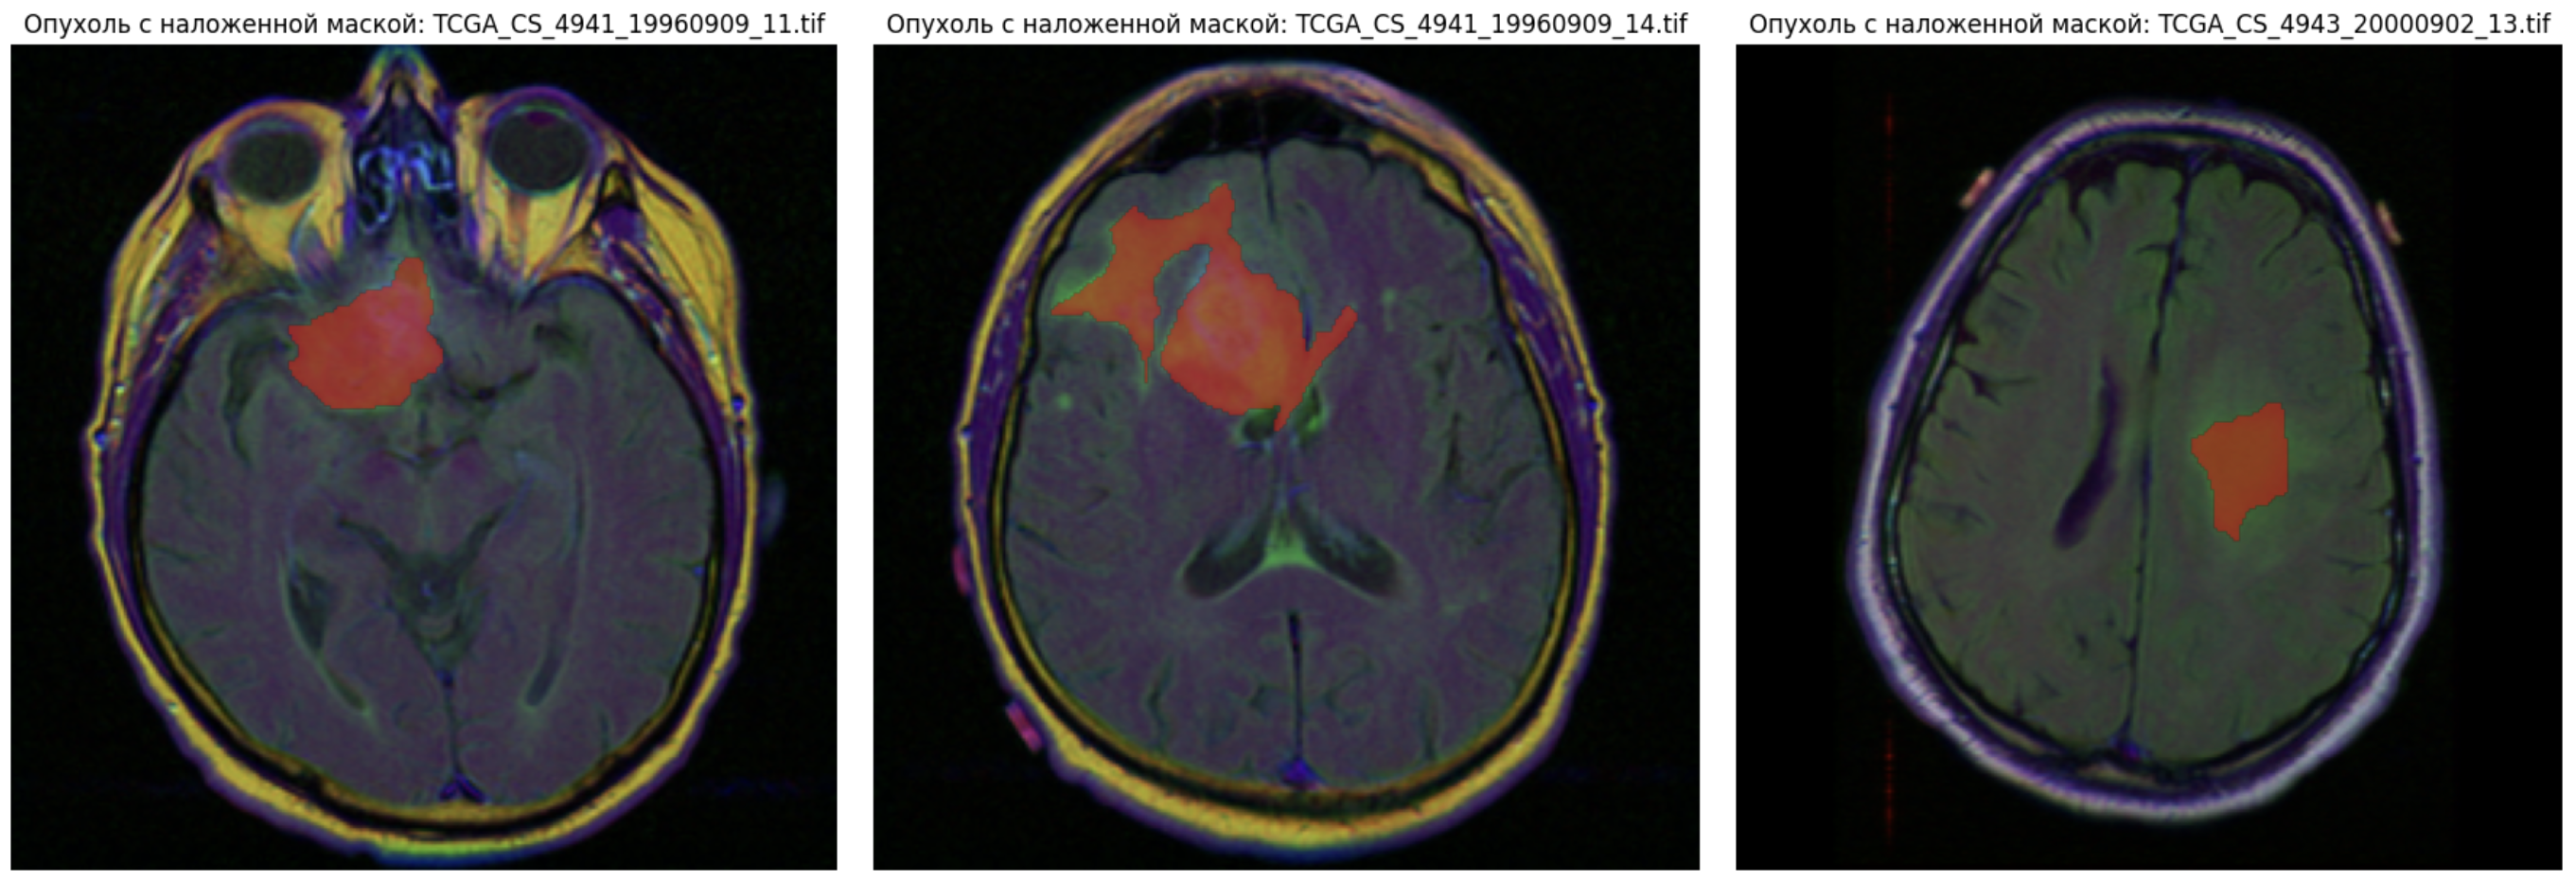
\includegraphics[width=\linewidth]{tumor_and_mask_2.png}
    \caption{Пример объединенного снимка с маской из датасета BraTS}
    \label{fig:tumor_and_mask_2}
  \end{minipage}
\end{figure}

\subsection{Замер IoU на датасете BraTS}

Теперь применим наш метод на новом датасете и посмотрим, как совпадают и расходятся предсказание масок и истинные маски. Для этого возьмем исходный снимок и подадим его на вход модели. Далее сравним выход модели с истинной областью опухоли. Алгоритм сегментации можно описать следующим образом:

\begin{enumerate}
    \item Загружаем МРТ-снимки из датасета BraTS вместе с соответствующими масками опухолей. Все маски преобразуем в бинарный формат (0 или 1). Дополнительно применим небольшое сглаживаение к данным, чтобы уменьшить влияние шума;

    \item Разделим каждое изображение на небольшие перекрывающиеся фрагменты (патчи). Далее каждый патч преобразуется в одномерный вектор, дополнительно для каждого патча сохраняем его позиция (индекс изображения и координаты);

    \item Для каждого патча находим его ближайших соседей, используя алгоритм k-ближайших соседей [30]. Мы будем вычислять локальное линейное представление окрестности каждого патча с помощью SVD (сингулярное разложение). В итоге наш алгоритм создаёт касательное пространство, которое аппроксимирует многообразие данных локально;
    
    \item Далее проиcходит вычисление форм связности: для каждой пары соседних патчей вычисляется матрица, представляющая переход между их касательными пространствами. В итоге формы связности описывают, как касательные пространства соотносятся между соседними точками данных;

    \item Следующим шагом вычисляем кривизну. Мы будем вычислять ее на основе отношения минимального и максимального собственных значений ковариационной матрицы. Ранее в работе мы описывали, что кривизна измеряет, насколько локальная окрестность отклоняется от плоского пространства, то есть высокая кривизна может указывать на аномальные области (потенциальные опухоли);

    \item Далее происходит вычисление голономии: для каждого патча будем созадвать случайные пути через соседние патчи и вычислять параллельный перенос. Голономия измеряет, насколько сильно меняется вектор при транспортировке по замкнутому пути, а значит большие значения голономии указывают на нерегулярности в структуре данных, то есть могут быть дополнительным индикатором наличия особенности в данных;

    \item Далее для каждого патча его соседи проецируются на его касательное пространство и затем реконструируются обратно, причем высокая ошибка реконструкции указывает на то, что патч плохо представляется локальной линейной моделью. Итого, мы комбинируем три метрики (кривизна, голономия, ошибка реконструкции) с заданными весами (считаем их гиперпараметрами) и вычисляем окончательный показатель аномальности для каждого патча;

    \item На последнем этапе нам необходимо преобразовать показатели аномальности отдельных патчей обратно в формат полного изображения. Для этого мы будем применять сглаживание с помощью Гауссова фильтра [31]. В итоге мы получаем карту аномалий, к которой можно применить адаптивную пороговую обработку, чтобы получить бинарную маску. Данную маску мы и будем сравнивать с истинной маской.
    
\end{enumerate}

После применения такого алгоритма мы получаем предсказанную маску, которую необходимо сравнить с истинной маской. Пример предсказанной маски можно увидеть на рисунке~\ref{fig:brain_tumor_segmentation_results}. Сравнивать маски мы будем через метрику IoU. 

\begin{figure}[ht]
  \centering
  \begin{minipage}[b]{0.9\linewidth} 
    \centering
    
\includegraphics[width=\linewidth]{brain_tumor_segmentation_results.png}
    \caption{Пример предсказанной маски для выделения опухоли}
    \label{fig:brain_tumor_segmentation_results}
  \end{minipage}
\end{figure}

Сначала визуализируем пересечение масок (рисунок~\ref{fig:detailed_segmentation_results}). Далее нам необходимо определить порог комбинированной метрики (кривизна, голономия, ошибка реконструкции), после достижения которого точка будет считаться аномалией (рисунок~\ref{fig:iou_vs_percentile}). После определения порога мы можем пересчитать маски с новым порогом. Итого, мы получили средний IoU 0.3211. Комбинируя этот результат со значениями метрик детекции особенностей на синтетических данных, можно сделать вывод, что метод хорошо справляется с задачей определения опухоли. Отдельно отметим, что на данном шаге мы имеем алгоритмический метод, а не, например, нейронную сеть или другой метод машинного обучения. Таким образом, в теории, объединив наш метод и методы машинного обучения, можно получить метод, который еще лучше справляется с задачей определения опухолей на МРТ-снимках.

\begin{figure}[ht]
  \centering
  \begin{minipage}[b]{0.9\linewidth} 
    \centering
    
\includegraphics[width=\linewidth]{/Users/dasidorov03/PycharmProjects/dploma_4_course/diploma_latex_text/graphics/detailed_segmentation_results.png}
    \caption{Пример пересечения истинной и предсказанной масок}
    \label{fig:detailed_segmentation_results}
  \end{minipage}
\end{figure}

\begin{figure}[ht]
  \centering
  \begin{minipage}[b]{0.9\linewidth} 
    \centering
    
\includegraphics[width=\linewidth]{/Users/dasidorov03/PycharmProjects/dploma_4_course/diploma_latex_text/graphics/iou_vs_percentile.png}
    \caption{График подбора порога комбинированной метрики (кривизна, голономия, ошибка реконструкции)}
    \label{fig:iou_vs_percentile}
  \end{minipage}
\end{figure}

\subsection{Добавление топологических и геометрических признаков в архитектуру U-Net для сегментации опухолей мозга}

На данном этапе мы имеем алгоритмический способ выделения особенностей в данных (в нашем случае выделения опухолей в мозге на МРт-снимках). 
Теперь попробуем использовать геометрический анализ как признаковый слой для обучения нейросетей. В качестве сети будем использовать U-Net [32].

Для реализации такого улучшения будем модифицировать стандартную архитектуру U-Net путем внедрения дополнительной ветви для обработки топологических и 
геометрических признаков. Известно, что стандартная U-Net представляет собой полносвязную сверточную нейронную сеть с энкодер-декодерной структурой и skip-connections между 
соответствующими уровнями. Данная модель работает только с входными изображениями, не имея механизмов для прямого учета топологических и геометрических характеристик 
обрабатываемых данных. Разработанная нами сеть расширяет стандартную архитектуру, добавляя параллельную ветвь обработки для карт топологических и 
геометрических признаков. Вместо исходной одной ветви мы будем использовать двойной входной поток. Его работу можно описать следующим образом: 
основная ветвь принимает стандартное RGB-изображение (3 канала), далее дополнительная ветвь принимает карту признаков (1 канал), содержащую предварительно 
вычисленные топологические и геометрические характеристики. Для обработки карты признаков независимо от основного изображения мы добавим отдельную последовательность сверточных блоков.
Итого, обе ветви имеют идентичную структуру понижающей дискретизации, чтобы обеспечить совместимость размерностей на этапе слияния.

\section{Итоги и дальнейшая работа}

Итого, у нас появился фреймворк\footnote{Код доступен по ссылке: \url{https://github.com/deouron/diploma_4_course}, дата обр. 01.06.2025}, который принимает на вход МРТ-снимок (пространство точек), а на выходе определяет, содержит ли этот снимок особенности и выводит изображения срезов снимка с выделенными особенностями. Мы убедились, что используемые методы показывают хорошие результаты в терминах метрик ROC–AUC и PR–AUC. Следующими этапами развития фреймворка можно выделить дальнейшее улучшение метода и, как следствие, метрик, а так же интеграцию фреймворка в инструменты для аналитики МРТ-снимков, например, в виде программы для врачей, в которую они могут загружать файл с результатами МРТ, а на выходе получать выделенные (если есть) особенности. 

\pagebreak
	
\newpage 
\printbibliography[heading=bibintoc] 

\addcontentsline{toc}{section}{Список литературы}

\begin{thebibliography}{0}

    \bibitem{1}\hypertarget{2}{}
 Chattopadhyay, Surajit, and Goutami Chattopadhyay. ``Modeling and prediction of monthly total ozone concentrations by use of an artificial neural network based on principal component analysis.'' Pure and Applied Geophysics 169 (2012): 1891-1908.

 	\bibitem{2}\hypertarget{2}{}
 Van der Maaten, Laurens, and Geoffrey Hinton. ``Visualizing data using t-SNE.'' Journal of machine learning research 9, no. 11 (2008): 2580-2584.

 	\bibitem{3}\hypertarget{2}{}
 Hastie, Trevor, Robert Tibshirani, Jerome H. Friedman, and Jerome H. Friedman. The elements of statistical learning: data mining, inference, and prediction. Vol. 2. New York: springer, 2009: 193-224.

 	\bibitem{4}\hypertarget{2}{}
 Roweis, Sam T., and Lawrence K. Saul. ``Nonlinear dimensionality reduction by locally linear embedding.'' science 290, no. 5500 (2000): 2323-2326.

 	\bibitem{5}\hypertarget{2}{}
 Tenenbaum, Joshua B., Vin de Silva, and John C. Langford. ``A global geometric framework for nonlinear dimensionality reduction.'' science 290, no. 5500 (2000): 2319-2323.

 	\bibitem{6}\hypertarget{2}{}
 Jolliffe, Ian T. ``Principal component analysis: a beginner's guide—I. Introduction and application.'' Weather 45.10 (1990): 375-382.

 	\bibitem{7}\hypertarget{2}{}
 Tenenbaum, Joshua B., Vin de Silva, and John C. Langford. ``A global geometric framework for nonlinear dimensionality reduction.'' Science 290.5500 (2000): 2319-2323.

 	\bibitem{8}\hypertarget{2}{}
 Van Der Maaten, Laurens, Eric O. Postma, and H. Jaap Van Den Herik. ``Dimensionality reduction: A comparative review.'' Journal of machine learning research 10.66-71 (2009): 13.

 \bibitem{9}\hypertarget{2}{}
 de Leeuw, Jan, and Willem Heiser. ``13 theory of multidimensional scaling.'' Handbook of statistics 2 (1982): 285-316.

 \bibitem{10}\hypertarget{2}{}
 Blei, David M., Andrew Y. Ng, and Michael I. Jordan. ``Latent dirichlet allocation.'' Journal of machine Learning research 3.Jan (2003): 993-1022.

 \bibitem{11}\hypertarget{2}{}
 McInnes, Leland, John Healy, and James Melville. ``Umap: Uniform manifold approximation and projection for dimension reduction.'' arXiv preprint arXiv:1802.03426 (2018).

 \bibitem{12}\hypertarget{2}{}
 Wasserman, Larry. ``Topological data analysis.'' Annual Review of Statistics and Its Application 5.1 (2018): 501-532.

 \bibitem{13}\hypertarget{2}{}
Ghrist, Robert. ``Barcodes: the persistent topology of data.'' Bulletin of the American Mathematical Society 45.1 (2008): 61-75.

 \bibitem{14}\hypertarget{2}{}
Edelsbrunner, Herbert, and John L. Harer. Computational topology: an introduction. American Mathematical Society, 2022.

 \bibitem{15}\hypertarget{2}{}
Singh, Gurjeet, Facundo Mémoli, and Gunnar E. Carlsson. ``Topological methods for the analysis of high dimensional data sets and 3d object recognition.'' PBG@ Eurographics 2 (2007): 091-100.

 \bibitem{16}\hypertarget{2}{}
François, Anton, and Raphaël Tinarrage. ``Train-Free Segmentation in MRI with Cubical Persistent Homology.'' arXiv preprint arXiv:2401.01160 (2024).

\bibitem{17}\hypertarget{2}{}
IXI Hammersmith Hospital Dataset. URL: \url{https://brain-development.org/ixi-dataset/} (дата обр. 27.01.2025).

\bibitem{18}\hypertarget{2}{}
Bauer, Ulrich. ``Ripser: efficient computation of Vietoris–Rips persistence barcodes.`` Journal of Applied and Computational Topology 5.3 (2021): 391-423.

\bibitem{19}\hypertarget{2}{}
Biasotti, S., Giorgi, D., Spagnuolo, M., & Falcidieno, B. (2008). ``Reeb graphs for shape analysis and applications``. Theoretical computer science, 392(1-3), 5-22.

\bibitem{20}\hypertarget{2}{}
Sun, J., Cieslak, M., Grafton, S., & Suri, S. (2015, November). ``A reeb graph approach to tractography``. In Proceedings of the 23rd SIGSPATIAL International Conference on Advances in Geographic Information Systems (pp. 1-4).

\bibitem{21}\hypertarget{2}{}
Diepeveen, W., Batzolis, G., Shumaylov, Z., & Schönlieb, C. B. (2024). ``Score-based pullback Riemannian geometry.`` arXiv preprint arXiv:2410.01950.

\bibitem{22}\hypertarget{2}{}
Huang, Jin, and Charles X. Ling. ``Using AUC and accuracy in evaluating learning algorithms.'' IEEE Transactions on knowledge and Data Engineering 17.3 (2005): 299-310.

\bibitem{23}\hypertarget{2}{}
Vemuri, Baba C., Amar Mitiche, and Jake K. Aggarwal. ``Curvature-based representation of objects from range data.'' Image and vision computing 4.2 (1986): 107-114.

\bibitem{24}\hypertarget{2}{}
Echeandia, Sebastian, and Patrick M. Wensing. ``Numerical methods to compute the coriolis matrix and christoffel symbols for rigid-body systems.'' Journal of Computational and Nonlinear Dynamics 16.9 (2021): 091004.

\bibitem{25}\hypertarget{2}{}
Lanczos, Cornelius. ``The splitting of the Riemann tensor.'' Reviews of Modern Physics 34.3 (1962): 379.

\bibitem{26}\hypertarget{2}{}
Wei, Guofang, and Will Wylie. ``Comparison geometry for the Bakry-Emery Ricci tensor.'' Journal of differential geometry 83.2 (2009): 337-405.

\bibitem{27}\hypertarget{2}{}
Pradhan, Srutarshi, Alex Hansen, and Bikas K. Chakrabarti. ``Failure processes in elastic fiber bundles.'' Reviews of modern physics 82.1 (2010): 499-555.

\bibitem{28}\hypertarget{2}{}
Rezatofighi H. et al. ``Generalized intersection over union: A metric and a loss for bounding box regression.'' Proceedings of the IEEE/CVF conference on computer vision and pattern recognition (2019): 658-666.

\bibitem{29}\hypertarget{2}{}
U.Baid, et al., ``The RSNA-ASNR-MICCAI BraTS 2021 Benchmark on Brain Tumor Segmentation and Radiogenomic Classification'', arXiv:2107.02314, 2021.

\bibitem{30}\hypertarget{2}{}
Peterson, Leif E. ``K-nearest neighbor.'' Scholarpedia 4.2 (2009): 1883.

\bibitem{31}\hypertarget{2}{}
Ito, Kazufumi, and Kaiqi Xiong. ``Gaussian filters for nonlinear filtering problems.'' IEEE transactions on automatic control 45.5 (2000): 910-927.

\bibitem{32}\hypertarget{2}{}
Ronneberger, Olaf, Philipp Fischer, and Thomas Brox. ``U-net: Convolutional networks for biomedical image segmentation.'' Medical image computing and computer-assisted intervention–MICCAI 2015: 18th international conference, Munich, Germany, October 5-9, 2015, proceedings, part III 18. Springer international publishing, 2015.

\end{thebibliography}
\end{document}
